\documentclass [11pt]{article}
\usepackage{setspace,amssymb,latexsym,amsmath,amscd,epsfig,amsthm}
\usepackage{array,color}
\usepackage[english]{babel}
\usepackage{makeidx}
\usepackage{booktabs}
\usepackage{apacite}

\newcommand{\fts}{financial time series}
\newcommand{\margincomment}[2][blue]{\marginpar{\begin{small}\begin{flushleft}\textcolor{#1}{#2}\end{flushleft}\end{small}}}

%\newcommand\citeA[1]{\cite{#1}} % If I don't use name-year, I need a \citeA tag.
\usepackage[left=2.5cm,top=2.5cm,right=4cm]{geometry}
%\usepackage{moreverb} % Used for line-numbered verbatim text listings.
\graphicspath{{./images/}}

\makeindex

% List of Examples Header
\newcommand\ecaption[1]{\addcontentsline{xmp}{example}{#1}}
\makeatletter \newcommand\listofexamples {\section*{Code Samples}\@starttoc{xmp}}
\newcommand\l@example[2] {\par\noindent#1~\dotfill\textmd{#2}\par} \makeatother
%

% Only make the document for the sections as needed
\includeonly{msf566-notes-1, msf566-notes-2,msf566-notes-3,msf566-notes-4,
msf566-notes-5, msf566-notes-6, msf566-notes-7,msf566-notes-8}%,msf566-notes-9}

% SOURCES
% http://faculty.chicagogsb.edu/ruey.tsay/teaching/bs41202/sp2008/
% http://faculty.chicagogsb.edu/ruey.tsay/teaching/fts2/

\begin{document}
\pagestyle{myheadings}
\markright{MSF 566 Lecture Notes}
\title{MSF 566 - Financial Time Series Analysis  \\ Lecture Notes}
\author{Andrew P. Acosta}
%\date{}.

\pagenumbering{roman}
\maketitle
\thanks{The following collection of notes is the work product and intellectual property of \mbox{Andrew P. Acosta}. It is shared freely with the assumption that they not be relied upon as a primary source of research. Any errors found are his alone. Please send any comments and advice on errors and omissions you found to the author at \texttt{andrew@acm.org}. \linebreak
\tiny{Document typeset using \AmS{}-\LaTeX{}.}}

\tableofcontents
\clearpage
\listoffigures

\pagebreak
\listoftables
%\clearpage
%\section*{List of Examples}

\pagebreak
\listofexamples
\clearpage

\numberwithin{equation}{section}
\numberwithin{figure}{section}
\numberwithin{table}{section}

\pagenumbering{arabic}
\section{Introduction}
\paragraph{Primary Text Reading.} \citeA[chap. 1]{tsay2005aft}\index{Tsay, Ruey}
\subsection{What is \fts{} analysis?}\index{time series!definition}
In general, a time series is a sequence of data points, usually measured at successive times, spaced at specific intervals. Time series analysis comprises methods that seek to understand the context of the data points to answer questions such as, ``What is this series telling me about whatever is generating this series?'', or to make \emph{forecasts} to predict future data points.
\marginpar{\begin{small}\begin{flushleft}\textcolor{blue}{Much of time series analysis is predicting future outcomes.}\end{flushleft}\end{small}}
Time series forecasting is the use of a model to forecast future events based on known past events: to forecast future data points before they occur. A good example might be forecasting a price of a share of stock based on its past performance.

Financial time series analysis is concerned with asset valuation and volatility over time. The state of the world today (\textit{e.g.} a stock price or interest rate) is affected in some way by the previous state, perhaps yesterday or two seconds ago. Similarly, the state of the world in the future is likely to be affected by the current state. This assumption allows some level of \emph{financial forecasting} using various methods of time series analysis.

There are three major outcomes of time series analysis, graphical analysis, autocorrelation, and trend behavior. We will briefly discuss how each is explored.

\paragraph{Graphical analysis.} When we view a time series in the form of time series plot, we may observe peaks and valleys. It may become apparent that a trend has developed by looking at the rising and falling of the line. Methods that analyze time series data graphically comprise \index{technical analysis}\emph{technical analysis} and a \index{exploratory data analysis}\emph{Exploratory Data Analysis}.

\paragraph{Autocorrelation.}\index{autocorrelation} We may want to measure the extend to which data points seem to rely upon previous points, or how random they seem to be. This type of analysis applies autocorrelation studies.

\paragraph{Trend behavior.} Some \fts{} exhibit trends which can be examined numerically. They may have some seasonal pattern, such that, for instance, their level will rise in summer and decline in winter.

\subsection{Review of matrices, statistics and probability }
\subsubsection{Descriptive Statistics}
This section is a brief review of inferential statistics and probability.  There will also be some review of linear algebra, the mathematics of matrices.

\marginpar{\begin{small}\begin{flushleft}\textcolor{red}{A working knowledge of statistics and matrix math is assumed.}\end{flushleft}\end{small}}
Descriptive statistics are used to describe the basic features of the data in a study. They provide simple summaries about the sample and the measures. Together with simple graphics analysis, they form the basis of virtually every quantitative analysis of data. Statistics such as mean, median, and standard deviation are descriptive.

Descriptive statistics are typically distinguished from \emph{inferential statistics}. With descriptive statistics we are simply describing what is or what the data shows. With inferential statistics, we are trying to reach conclusions that extend beyond the immediate data alone. For instance, we use inferential statistics to try to infer from the sample data what the population might think. Or, we use inferential statistics to make judgments of the probability that an observed difference between groups is a dependable one or one that might have happened by chance in this study. Thus, we use inferential statistics to make inferences from our data to more general conditions; we use descriptive statistics simply to describe what's going on in our data.

Every time we try to describe a large set of observations with a single indicator we run the risk of distorting the original data or losing important detail. For this reason, statistics such as kurtosis and skewness are helpful in describing a frequency distribution with respect to a normal distribution.

The normal distribution is a histogram depicting the probability of a number with respect to its distance from a mean of zero across a range $(- \infty , \infty)$.

\begin{equation}
\phi(z) = \frac{1}{\sqrt{2 \pi}} \exp(-z^2/2), \quad - \infty < z < \infty
\label{eq:pdf}
\end{equation}

For instance,  \eqref{eq:pdf} is the equation that produces Figure~\ref{figure:pdf}.
The cumulative distribution \eqref{eq:cdf} is depicted in Figure~\ref{figure:cdf}.

\begin{equation}
\phi(z) = \int^z_{-\infty} \frac{1}{\sqrt{2 \pi}} \exp(-z^2/2), \quad - \infty < z < \infty
\label{eq:cdf}
\end{equation}

\begin{figure}[t]
  \centering
  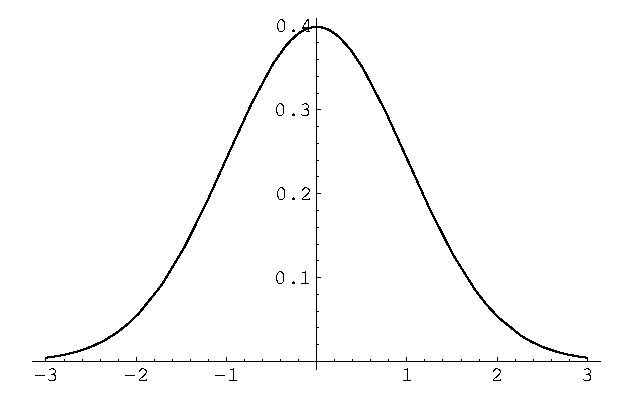
\includegraphics[scale=.75]{pdf}
  \caption{Normal Probability Density}
  \label{figure:pdf}
\end{figure}

\begin{figure}[t]
  \centering
  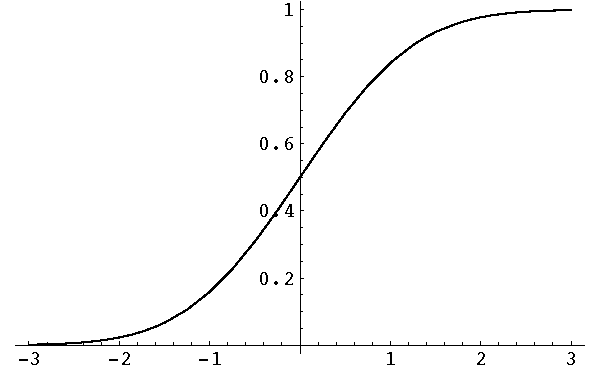
\includegraphics[scale=.75]{cdf}
  \caption{Normal Cumulative Distribution}
  \label{figure:cdf}
\end{figure}

A great deal of statistical analysis comes from the normal distribution. Being able to calculate the values of specific ranges in the distribution is essential to understanding descriptive statistics.

\subsubsection{Sampling and Validity}\index{sampling}\index{sampling!validity}
Sampling is the process of selecting units (\textit{e.g.}, people, organizations) from a population of interest so that by studying the sample we may fairly generalize our results back to the population from which they were chosen. We begin by covering some of the key terms in sampling like ``population'' and ``sampling frame.'' Then, because some types of sampling rely upon quantitative models, we talk about some of the statistical terms used in sampling.

\paragraph{Random Sample.} \index{sampling!random}\index{recursion|see{recursion}}
Since it is not practical or even possible in many cases, to gather all data from a population, gathering a sample is preferred. However, the method by which a sample is chosen is very important and will affect the results of analysis. One of the easiest sampling methods is creating a \emph{random sample}.

How do we select a simple random sample? Assume that we are doing some research in equity analysis using a specific price forecasting method. First, we have to get the sampling frame organized. To accomplish this, we have to define the universe of stocks that are eligible for study. Next, we actually draw the sample using some random number assigned to each stock. If we are studying 100 stocks in our sample of perhaps 5,000 stocks. Then, the sampling fraction is $f = n/N = 100/5000 = .02$ or 2\%. To actually draw the sample, we have several options. We could print the list of 5,000 stocks, tear them into separate strips, put the strips in a box, and pull out the first 100. This mechanical procedure is tedious and the quality of the sample would depend on how thoroughly we mixed them up and how randomly we reached in.

A better procedure would be to use a random number generator that picks a number from 1 to 5,000, such as the following MATLAB code,\\

\ecaption{Generating 5,000 Random Integers}
\texttt{my\_sample=floor(5000*rand(1,100));} \\

However, this method does \emph{not} guarantee that the numbers generated will be unique, but it is a start. Simple random sampling is simple to accomplish and is easy to explain to others. Because simple random sampling is a fair way to select a sample, it is reasonable to generalize the results from the sample back to the population. Simple random sampling is not the most statistically efficient method of sampling and we may, just because of the luck of the draw, not get good representation of subgroups in a population. To deal with these issues, we have to turn to other sampling methods.

\paragraph{Systematic Sample.} \index{sampling!systematic}
Another random selection method is to pick every $k$th item in a population.
Here are the steps to achieve a systematic random sample,
\begin{enumerate}
\item number the units in the population from 1 to $N$
\item decide on the $n$ (sample size) that we need
\item $k = N/n = $ the interval size
\item randomly select an integer between 1 to $k$
\item select every $k$th unit
\end{enumerate}

All of this will be much clearer with an example. Assume that we have a population that only has $N=100$ items in it and that we want to take a sample of $n=20$. To use systematic sampling, the population must be listed in a random order. The sampling fraction would be $f = 20/100 = 20\%$. In this case, the interval size, $k$, is equal to $N/n = 100/20 = 5$. Now, we select a random integer from 1 to 5. In our example, imagine that we chose 4. Now, to select the sample, we start with the 4th unit in the list and take every $k$th unit (every 5th, because $k$=5). We would be sampling units 4, 9, 14, 19, \ldots, 100 and we would have 20 units in our sample.

For this to work, it is essential that the units in the population are randomly ordered, at least with respect to the characteristics we are measuring. Systematic random sampling is fairly easy to do. We only have to select a single random number to start things off. It may also be more precise when selecting the sample size $n$ than a simple random sampling, which uses a random number generator that is not guaranteed to be unique.

\paragraph{Stratified Sample.} \index{sampling!stratified}
This is a sample within a sample because a sample is drawn, and then a sample from within that is drawn. Stratified random sampling, also sometimes called \emph{proportional} or \emph{quota random sampling}, involves dividing our population into homogeneous subgroups and then taking a simple random sample in each subgroup.

In more formal terms, we divide the population into non-overlapping groups (\textit{i.e.}, strata) $N_1, N_2, N_3, \ldots, N_i$, such that $N_1 + N_2 + N_3 + \cdots + N_i = N$. Then we select a simple random sample of $f = n/N$ in each strata.

There are several major reasons why we might prefer stratified sampling over simple random sampling. First, it assures that we will be able to represent not only the overall population, but also key subgroups of the population, especially small minority groups. If we want to be able to talk about subgroups, this may be the only way to effectively assure we will be able to.

If the subgroup is extremely small, we can use different sampling fractions, $f$ within the different strata to randomly over-sample the small group (although we will have to weight the within-group estimates using the sampling fraction whenever we want overall population estimates). When we use the same sampling fraction within strata we are conducting proportionate stratified random sampling. When we use different sampling fractions in the strata, we call this \emph{disproportionate stratified random sampling}.

Second, stratified random sampling will generally have more statistical precision than simple random sampling. This will only be true if the strata or groups are homogeneous. If they are, we expect that the variability within-groups is lower than the variability for the population as a whole. Stratified sampling capitalizes on that fact.

For example, we want to test a trading strategy that works well for stocks of consumer staples, automotive, and leisure industry. We have three populations. Let us say that the population of stocks for our study can be divided into three groups: consumer staples, automotive, and leisure. Furthermore, let us assume that both the automotive and the leisure stocks are relatively few within the population (10\% and 5\% respectively). If we just did a simple random sample of $n=100$ with a sampling fraction of 10\%, we would expect by chance alone that we would only get 10 and 5 persons from each of our two smaller groups. And, by chance, we might get fewer than that.

If we stratify, we can do better. First, let us determine how many stocks we want to have in each group. Let us say we still want to take a sample of 100 from the population of 1,000 stocks. But we think that in order to say anything about subgroups we will need at least 25 cases in each group. So, we will sample 50 consumer staples, 25 automotive, and 25 leisure stocks. We know that 10\% of the population, or 100 stocks, are automotive. If we randomly sample 25 of these, we have a within-stratum sampling fraction of $25/100 = 25\%$. Similarly, we know that 5\% or 50 stocks are leisure. So our within-stratum sampling fraction will be $25/50 = 50\%$. Finally, by subtraction we know that there are 850 consumer staples stocks. Our within-stratum sampling fraction for them is $50/850 =  5.88\%$. Because the groups are more homogeneous within-group than across the population as a whole, we can expect greater statistical precision (less variance). And, because we stratified, we know we will have enough cases from each group to make meaningful subgroup inferences.

\begin{table}[htbp]
   \centering
   \begin{tabular}{@{} lrcl @{}}
      \toprule
      \multicolumn{4}{c}{Stratified Sample} \\
      \hline
       Type    & within pop. & sample size & within-stratum sample \\
      \hline
      consumer staples  & 85\% & 50 & 50/850 = 5.88\% \\
      automotive   & 10\% & 25 & 25/100 = 25\% \\
      leisure industry & 5\%  & 25 & 25/50 = 50\% \\
      \bottomrule
   \end{tabular}
   \caption{Stratified Sample Selection}
   \label{tab:strat-sample}
\end{table}

\paragraph{Convenience Sample.}\index{sampling!convenience}
A convenience sample is one where the items sampled from the population are chosen for their easy access. For instance, a consumer survey conducted by asking the first 100 people who walk into a particular bank one morning is a convenience sample. Those not going to that bank on that morning are not part of the sample. This might be an important issue, or it might not be, depending upon the purpose of the survey. Choosing 100 stocks for analysis based upon the fact that the analyst has heard of them is also a convenience sample because it ignores the perhaps thousands of stocks unknown to the analyst.

\paragraph{Validity.}\index{validity!external}
\emph{External validity} is related to generalizing.
\margincomment{Validity refers to the approximate truth of propositions, inferences, or conclusions}
External validity refers to the approximate truth of conclusions that involve generalizations. In other words, external validity is the degree to which the conclusions in a study would hold for other persons in other places and at other times.

In science there are two major approaches to how we provide evidence for a generalization. The first approach is the \emph{Sampling Model}.\index{validity!sampling}
In the sampling model, we start by identifying the population to generalize to. Then, we draw a fair sample from that population and conduct research with the sample. Finally, because the sample is representative of the population, one can automatically generalize results back to the population. However, there are several problems with this approach.

First, perhaps we do not know at the time of the study who we might ultimately like to generalize to. Second, we may not be easily able to draw a fair or representative sample. Third, it is impossible to sample across all times that we might like to generalize to (like next year).

The second approach to generalizing is the \emph{Proximal Similarity Model}.\index{validity!proximal similarity}
Under this model, we begin by thinking about different generalizability contexts and developing a theory about which contexts are more like our study and which are less so. For instance, we might imagine several settings that have people who are more similar to the people in our study or people who are less similar. This also holds for times and places.

When we place different contexts in terms of their relative similarities, we can call this implicit theoretical a gradient of similarity. Once we have developed this proximal similarity framework, we are able to generalize. How? We conclude that we can generalize the results of our study to other persons, places or times that are \emph{more like} (that is, more proximally similar) to our study. Notice that here, we can never generalize with certainty -- it is always a question of more or less similar.

\paragraph{Threats to External Validity.}
A threat to external validity is an explanation of how we might be wrong in making a generalization. For instance, we conclude that the results of our study (which was done in a specific place, with certain types of people, and at a specific time) can be generalized to another context (for instance, another place, with slightly different people, at a slightly later time). There are three major threats to external validity because there are three ways we could be wrong -- people, places or times.

Our critics could argue that the results of our study are due to the unusual type of people who were in the study. Or, they could argue that it might only work because of the unusual place we did the study in (perhaps we did our educational study in a college town with lots of high-achieving educationally-oriented students). Or, one might suggest that we did our study in a peculiar time. For instance, if we did an interest rate study the week after the Federal Reserve issues the well-publicized results of the latest rate change, we might get different results than if we had done it the week before.

\paragraph{Improving External Validity.}
\margincomment[red]{External validity (\emph{ability to generalize}) will be stronger the more we replicate our study.}
How can we improve external validity? One way, based on the sampling model, suggests that we do a good job of drawing a sample from a population. For instance, we should use random selection, if possible, rather than a \emph{nonrandom} procedure.

A second approach would be to use the theory of proximal similarity more effectively. How? Perhaps we could do a better job of describing the ways our contexts and others differ, providing lots of data about the degree of similarity between various groups of people, places, and even times. We might even be able to map out the degree of proximal similarity among various contexts with a methodology like concept mapping. Perhaps the best approach to criticisms of generalizations is simply to show them that they are wrong -- do the study in a variety of places, with different people and at different times.

Once we identify the theoretical and accessible populations, we have to get a list of the members of the accessible population. The listing of the accessible population from which we draw our sample is called the \emph{sampling frame}. If we were doing a performance survey of S\&P 500 stocks, then the stocks within the index would be our sampling frame. Getting that listing is simply a matter of going to a Bloomberg terminal\index{Bloomberg}
and obtaining the list. Other studies may be as simple, such as studying the rate of inflation on the money supply, for instance. However, preparing sample data of credit default swaps, for which the data is very difficult to obtain, also is difficult to compare to other swaps. This is a generally inaccessible population.

People often confuse what is meant by \emph{random selection} with the idea of \emph{random assignment}. You should make sure that you understand the distinction between random selection and random assignment. Random selection is the method by which the sample is selected, and random assignment is the method by which those samples are assigned to a test group or to a control group.

\subsubsection{Inferential Statistics}
With inferential statistics, we are trying to reach conclusions that extend beyond the immediate data alone. For instance, we use inferential statistics to try to infer from the sample data what the population might signify. Or, we use inferential statistics to make judgments of the probability that an observed difference between groups is a dependable one or one that might have happened by chance in this study. Thus, we use inferential statistics to make inferences from our data to more general conditions; we use descriptive statistics simply to describe what is going on in our data.
\marginpar{\begin{small}\begin{flushleft}\textcolor{blue}{Inferential statistics help make predictions and judgements}\end{flushleft}\end{small}}

Most of the major inferential statistics come from a general family of statistical models known as the General Linear Model. This includes the $t$ test, Analysis of Variance (ANOVA), Analysis of Covariance (ANCOVA), regression analysis, and many of the multivariate methods like factor analysis, multidimensional scaling, cluster analysis, and discriminant function analysis.

The purpose of these statistical tests is to conduct an experiment. Is a certain procedure effective in forecasting rates? Is there a significant difference between two samples?

\subsection{Statistical Inference}\index{statistical inference}
When we make some conclusion from a data sample we obtained, we draw an inference about a population based on some statistical inference method.
\margincomment[red]{A statistic is drawn from a sample. A parameter is contained in the population.}
We may be attempting to predict one of the following,
\begin{itemize}
\item point estimate: \index{point estimation} we are trying to determine a specific number
\item interval estimate:\index{interval estimation} we are tying to obtain a \emph{confidence interval}
\item hypothesis test:\index{hypothesis test}  we run a statistical significance test to determine if a sample belongs in the population
\end{itemize}

\subsubsection{Point Estimation}\index{point etimation}
Point estimation involves the use of sample data to calculate a single value (known as a \emph{statistic}) which is to serve as a ``best guess'' for an unknown (fixed or random) population \emph{parameter}.
One of the best known methods of point estimation is linear regression using the method of ordinary least squares. For example, Figure~\ref{figure:pt-est} is a linear regression through a scatterplot.

In most types of regression analysis, linear or otherwise, we are getting a point estimate through a plane, or more simply, a line that predicts points along the line.
\begin{figure}[t]
  \centering
  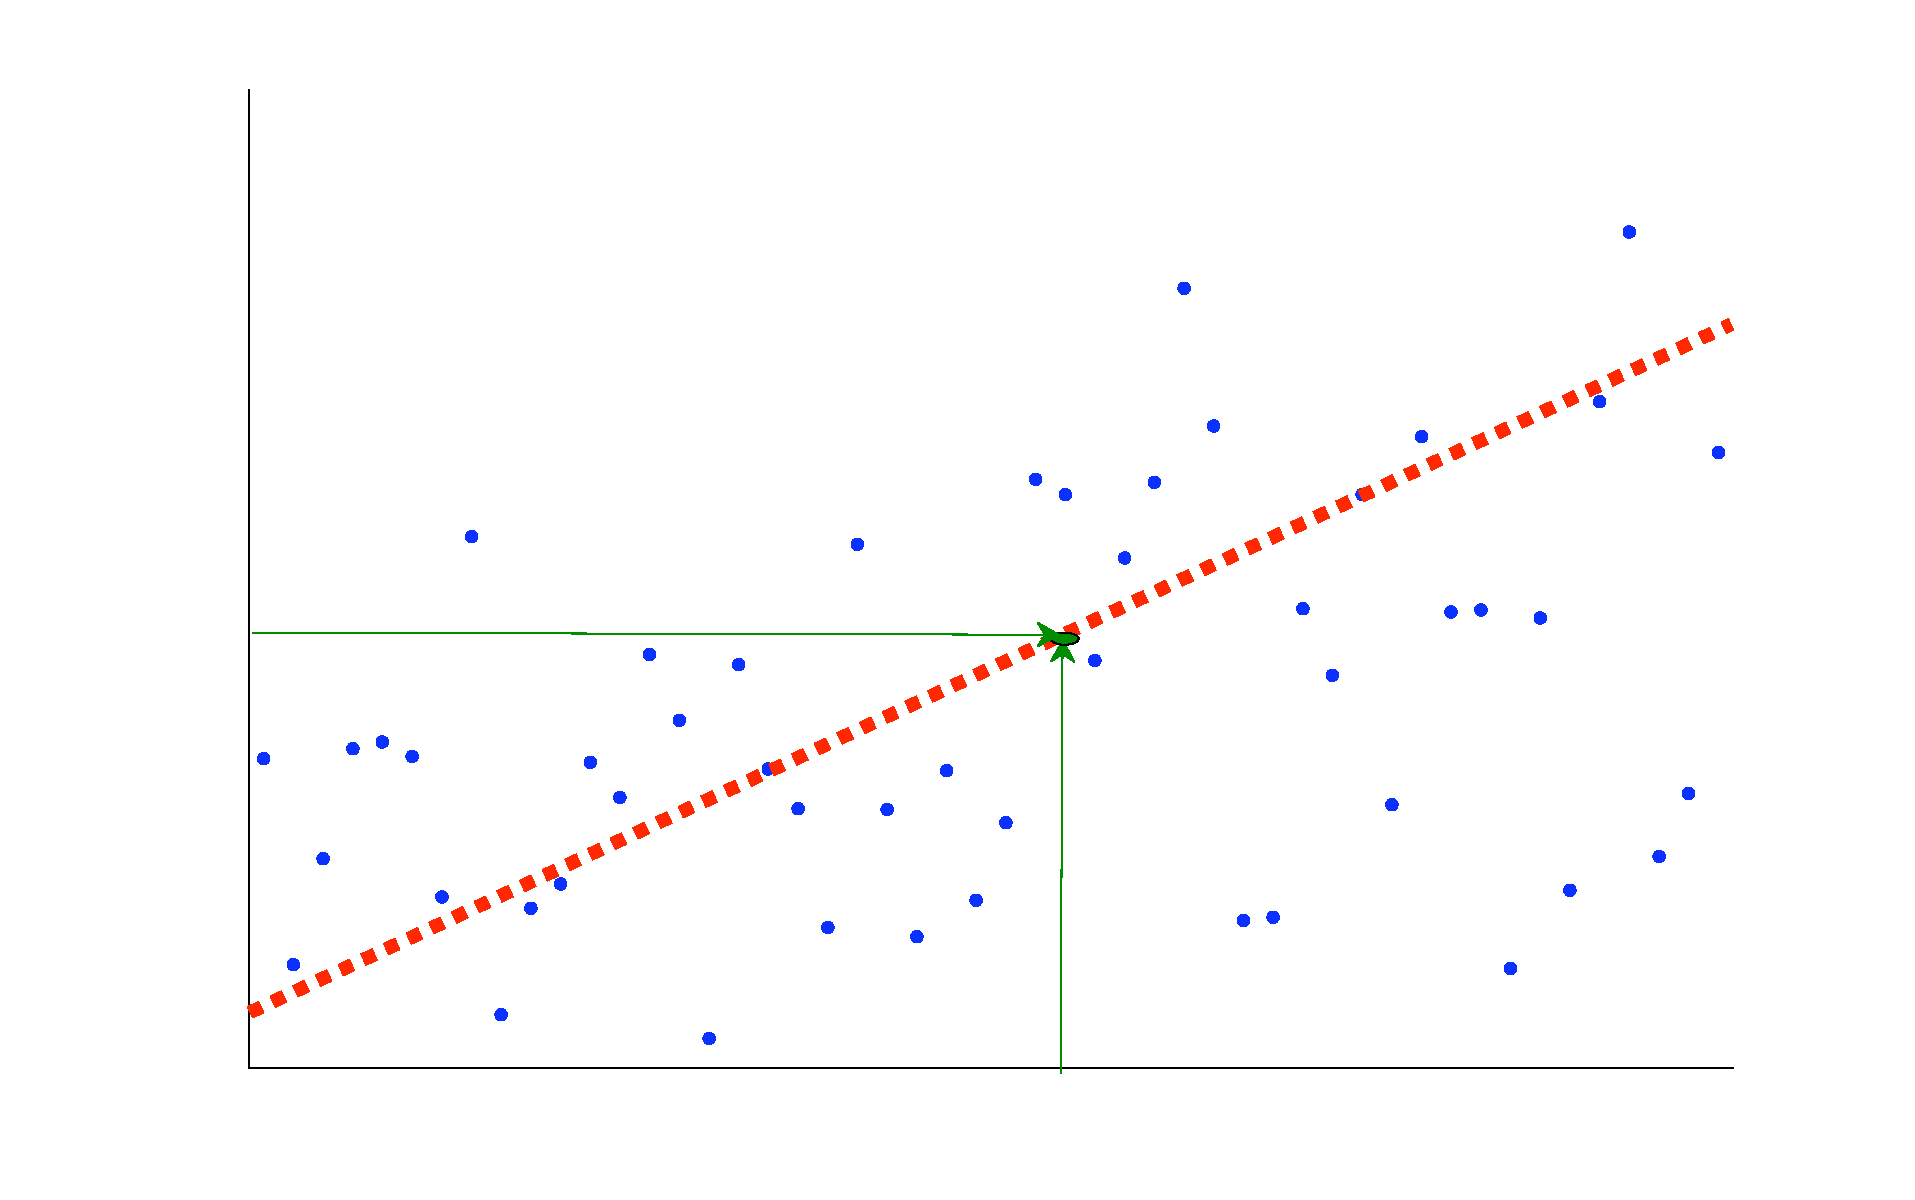
\includegraphics[scale=.35]{pt-est}
  \caption[Scatterplot and OLS Regression]{Scatterplot and OLS regression showing a single point estimate which is at the ($x$, $y$) coordinates marked by arrows.}
  \label{figure:pt-est}
\end{figure}

\subsubsection{Interval Estimation}\index{interval estimation}
Interval estimation is the use of sample data to calculate an interval of probable values of an unknown population parameter. The most prevalent forms of interval estimation are \emph{confidence intervals}. Because samples are taken from a population with a distribution, such as a normal distribution (Figure~\ref{figure:pdf}), it is possible that the sample does not accurately describe the population. If a point estimate is taken from one of the two tails of the distribution, it certainly would not represent the mean of the population.

An interval estimate provides some information about the accuracy of the sample and it represents a range of likely values. For instance, we can obtain a 95\% confidence interval, meaning that we have a 95\% confidence that our population mean $\mu$ is contained in our interval. To create the interval we calculate,
\begin{eqnarray}
P \big(-z< \frac{\bar{Y}-\mu}{1/\sqrt{n}}<z \big)&=&.95 ; \quad z= 1.96 \label{eq:conf-int} \\
P \big(-1.96< \frac{\bar{Y}-\mu}{1/\sqrt{n}}<1.96 \big)&=&.95, \notag
\end{eqnarray}
which gives us an interval estimate of $\Big[\bar{y}-1.96/\sqrt{n},\bar{y}+1.96/\sqrt{n} \Big]$, or $\bar{y} \pm 1.96/\sqrt{n}$.

\subsubsection{Hypothesis Testing}\index{hypothesis test}\label{hyp-test}
A hypothesis test is a method of making statistical decisions about experimental data that answers the question of how well the findings fit the probability that chance factors alone might be responsible. This is done by asking a hypothetical question and performing a test that compares a sample to its population.

To set up a hypothesis test, we begin with a \emph{null hypothesis}. For example, we want to test a cereal-filling machine at a factory \cite[pp. 332--358]{levine-2004sme}. Our test is to determine if the machine is pouring out the expected weight of 368 grams into each box of cereal.

We have a sample of 25 cereal boxes, and we want to test if the machine is filling properly based on the average weight from our sample. To do so, we must state a null hypothesis,
\[
H_0 : \mu=368,\index{null hypothesis}\index{H0@$H_0$|see{null hypothesis}}
\]
and an alternative hypothesis as,
\[
H_1 : \mu \ne 368. \index{alternative hypothesis}\index{H1@$H_1$|see{alternative hypothesis}}
\]

The cereal in the 25 boxes is weighed, and its average (\emph{mean} weight) is found to be 372.5 grams. We know that, on average, the machine has poured too much cereal, some boxes may have too much, others too little. The real question is, ``Is 372.5 grams per box \emph{close enough} to consider the cereal machine to be working?''

Before we can say what is close enough, we need to know how much variance to expect from the cereal-filling machine, and we need to establish a threshold of how much difference is acceptable. Because we are using only a sample, it is possible to make a testing error. We are given the population standard deviation $\sigma=15$.

\paragraph{Hypothesis Errors.}There are two kinds of hypothesis errors we can make,
\begin{description}
\item[Type I Error] This occurs when rejecting a null hypothesis that should not have been rejected. The probability of a Type I error is defined as the \emph{level of significance}\index{level of significance} which uses the symbol $\alpha$.\index{alpha@$\alpha$ (alpha)|see{level of significance}}
\item[Type II Error] This occurs when not rejecting the null hypothesis when we should have. The probability of a Type II error is denoted by the symbol $\beta$.\index{beta@$\beta$ (beta)!in hypothesis}
\end{description}

\begin{table}[htbp]
   \centering
   \begin{tabular}{@{} lcc @{}}
      \toprule %\hline
      \multicolumn{3}{r}{Actual State of Population} \\
      \hline
       Decision    & $H_0$ is True & $H_0$ is False\\
      \hline
      Reject $H_0$  & Type I Error & Correct Decision \\
      & Probability: $\alpha$ & Probability: $1- \beta$  \\
      \\
      Do not Reject $H_0$   & Correct Decision  & Type II Error \\
      & Probability: $1-\alpha$ & Probability: $\beta$  \\
      \bottomrule %\hline
   \end{tabular}
   \caption{Hypothesis Testing Errors}
   \label{tab:hyp-test-err}
\end{table}

\marginpar{\begin{small}\begin{flushleft}\textcolor{blue}{Two-sided hypothesis test divides the $\alpha$ equally on both tails.}\end{flushleft}\end{small}}
A hypothesis test can be one-sided or two-sided, depending upon the alternative hypothesis. A two-sided hypothesis is nondirectional, such as $H_1: \theta \ne \theta_0$, which we see in Figure~\ref{figure:rej-region2}. A one-sided hypothesis is only concerned with one direction or the other. The alternative hypothesis $H_1: \theta < \theta_0$ is a \emph{left-directional test}, as seen in Figure~\ref{figure:rej-region}, and $H_1: \theta > \theta_0$ is a \emph{right-directional test}.

Our cereal machine should not pour too much or too little cereal. We have established a two-sided hypothesis test. We will establish our level of significance of .05 or 5\%.

\begin{figure}[t]
  \centering
  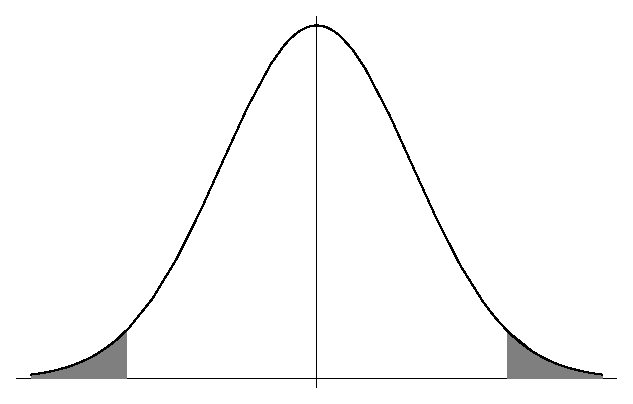
\includegraphics[scale=.7]{rej-region2}
  \caption{Two-Sided Region of Rejection}
  \label{figure:rej-region2}
\end{figure}
\begin{figure}[t]
  \centering
  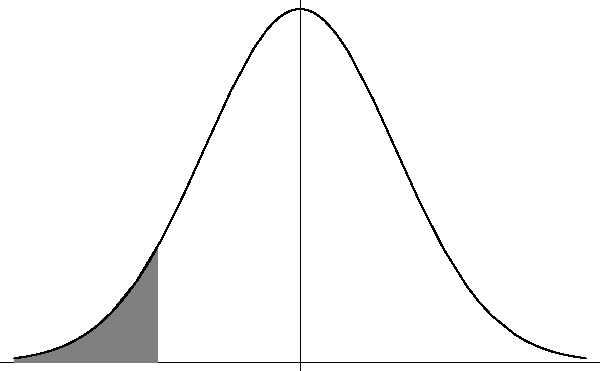
\includegraphics[scale=.7]{rej-region}
  \caption{One-Sided Region of Rejection}
  \label{figure:rej-region}
\end{figure}

Next, we need a \emph{confidence coefficient}, which is denoted by $1-\alpha$. In our cereal test, the confidence coefficient is .95. Our \emph{region of non-rejection} therefore is .95, which implies that our \emph{region of rejection} is .025 on either side of the distribution in Figure~\ref{figure:rej-region2} for a total of .05. We must convert our rejection threshold value into a \emph{critical value} by locating where on the normal distribution the region ending at .025 is located. We can obtain the critical value in MATLAB using,
\ecaption{Obtaining Critical Value}\texttt{cv=norminv((1-0.025),0,1)}, which gives  us 1.96. Since this is a two-tailed test, our critical value is $\pm 1.96$.

Now that we know where the sample mean should lie within the distribution, we need to calculate the \emph{z-test statistic} which determines the sample mean's position relative to the population. The $z$-test statistic is obtained by,
\begin{equation}
\boxed{\quad z = \frac{\bar{X} - \mu}{\frac{\sigma}{\sqrt{n}}}. \quad}
\label{eq:z-test}
\end{equation}
We have the numbers we need to proceed, $\bar{X}=372.5, \mu=368, \sigma=15, n=25$, and we can use \eqref{eq:z-test} to generate a $z$-test statistic,\index{z@$z$-test statistic}
\[
z = \frac{372.5 - 368}{15/\sqrt{25}} = 1.5.
\]

Since our $z$-test statistic is within the region of non-rejection ($-1.96 < z < 1.96$), we state that \emph{there is insufficient evidence to claim that our sample mean is different from the population mean}. The difference in the weight of the cereal is ``close enough.''

\subsection{Linear Algebra}\label{linear-algebra}\index{matrix math|see{linear algebra}}\index{linear algebra}\index{MATLAB}\index{R language}
To perform matrix operations, We will be using MATLAB, and R, which allow us to perform matrix multiplication and other related operations, but it is important to remember is how to multiply two matrices.
\margincomment{The size of a matrix is described by number of rows $\times$ columns}
For example, matrix $\mathbf{A} \times \mathbf{B}$ where,
\begin{eqnarray}
	\label{eq:matmult}
\mathbf{A} &=& \notag
	\begin{bmatrix}
	1 & 2 & 3 \\
	4 & 5 & 6 \\
	\end{bmatrix} \\
\mathbf{B}&=&  \notag
	\begin{bmatrix}
	10 & 20 \\
	30 & 40 \\
	50 & 60 \\
	\end{bmatrix} \\
\\ \notag
\mathbf{A} \mathbf{B}&=&
	\begin{bmatrix}
	220 & 280 \\
	490 & 640 \\
	\end{bmatrix},
\end{eqnarray}

or, more generally,
\begin{eqnarray}
	\label{eq:matmultnum}
\mathbf{A} &=& \notag
	\begin{bmatrix}
	a_{11} & a_{12} & a_{13} \\
	a_{21} & a_{22} & a_{23} \\
	\end{bmatrix} \\
\mathbf{B}&=&  \notag
	\begin{bmatrix}
	b_{11} & b_{12} \\
	b_{21} & b_{22} \\
	b_{31} & b_{32} \\
	\end{bmatrix} \\
\\ \notag
\mathbf{A} \mathbf{B}&=&
	\begin{bmatrix}
	a_{11} b_{11} + a_{12} b_{21} + a_{13} b_{31} & a_{11} b_{12} + a_{12} b_{22} + a_{13} b_{32} \\
	a_{21} b_{11} + a_{22} b_{21} + a_{23} b_{31} & a_{21} b_{12} + a_{22} b_{22} + a_{23} b_{32} \\
	\end{bmatrix}.
\end{eqnarray}

Only matrices of specific sizes may be multiplied.

The multiplication in \eqref{eq:matmult} and \eqref{eq:matmultnum} is allowed because $\mathbf{A}$ is a $2 \times 3$ matrix, $\mathbf{B}$ is a $3 \times 2$ matrix, and the number of columns in $\mathbf{A}$ must equal the number of rows in $\mathbf{B}$. The expression,
\[
\mathbf{A_{[m \times n]}} \times \mathbf{B_{[p \times q]}}
\]
requires that $n=p$. The resulting matrix will be of size $[m \times q]$.

\margincomment[red]{The law of commutativity does \emph{not} apply to matrices.}
It is important to note that the order the two matrices is multiplied is very important. The result will most likely be very different, if it can be computed at all.
\[
\boxed{\quad \mathbf{AB} \neq \mathbf{BA} \quad}
\]

Often, some calculations require a matrix to be \emph{transposed}. This is simply a rotation of columns to rows, as in the example,
\begin{eqnarray}
\mathbf{A} &=& \notag
	\begin{bmatrix}
	a_{11} & a_{12} & a_{13} \\
	a_{21} & a_{22} & a_{23} \\
	\end{bmatrix} \\
\mathbf{A^{T}} &=& \notag
	\begin{bmatrix}
	a_{11} & a_{21} \\
	a_{12} & a_{22} \\
	a_{13} & a_{23} \\
	\end{bmatrix}
\end{eqnarray}

Let us examine how MATLAB evaluates \eqref{eq:matmult}. A data structure, such as an array or matrix, is enclosed within brackets. The data elements may be comma-separated or separated by a space. A semicolon delimits a new row.
\ecaption{Matrix Multiplication in MATLAB}
\begin{verbatim}
    A=[1 2 3; 4 5 6];
    B=[10 20; 30 40; 50 60];
    A*B

    ans =
       220   280
       490   640
\end{verbatim}
Compare \eqref{eq:matmult} to the MATLAB syntax above to see how the expression is coded. The semicolon at the end of a line suppresses printing of an expression to the Command Window, but the values are displayed in the Workspace.

Now, we will perform the same matrix multiplication using the R language.
\index{R language}
\ecaption{Matrix Multiplication in R}
\begin{verbatim}
    A<-matrix(c(1,4,2,5,3,6),2,3)
    B<-matrix(c(10,30,50,20,40,60),3,2)
    A %*% B
    
         [,1] [,2]
    [1,]  220  280
    [2,]  490  640
\end{verbatim}
One difference you may notice in the syntax is that MATLAB accepts matrix elements row-by-row, but R accepts them by columns, and we specify the number of rows and columns. Also, R requires the \texttt{\%*\%} operator for matrix multiplication. 


%\nocite{bollerslev1987cht}
%\typeout{nocite being used for no reason by Andrew.}
\section{Introduction to MATLAB and R}
\paragraph{Primary Text Reading.}
\texttt{http://www.r-project.org/about.html} \\
\texttt{http://cran.r-project.org/manuals.html} \linebreak
\textit{especially} \textbf{An Introduction to R} and \textbf{R Data Import/Export}
\index{MATLAB}\index{R language}

\subsection{Statistical Computing}
Many analytical methods are highly complex, involving multiple calculations, formulas, and graphics.\footnote{A good resource for exploring more on statistical computing is the American Statistical Association website for \textbf{Statistics Computing and Graphics} at, \texttt{http://stat-computing.org/}}
Statistical computing, also known as computational statistics may also be used to refer to computationally-intensive statistical methods including resampling methods, Markov chain Monte Carlo methods, local regression, kernel density estimation and generalized additive models.

Both MATLAB and R are statistical computing environments; they both have broad support in the quantitative finance community as well as having a large number of libraries or packages that contain specialized functions. In class, we will attempt to be as platform-independent as possible, as well as trying to avoid proprietary data formats, such as Microsoft Excel. All data sets will be comma-delimited, or tab/space delimited so that they can be used by any editor and work equally well in MATLAB, R, or any other statistical software package.

\subsubsection{MATLAB}
To MATLAB, \emph{everything} is a matrix, including a single value, a \emph{scalar}. MATLAB has matrix math processing built in as well as a rich set of programming features for data access, graphical user interface, and mathematical computation and simulation. Despite its long list of features, MATLAB is very easy to use and can produce meaningful results in a short time span. MATLAB has robust file processing capability, meaning that very large datasets, perhaps amounting to millions of items, pose no difficulty. Having numerous functions already available and tested make MATLAB a good environment for rapid development of models. Writing programs in a language like C++ requires considerably more commitment of time and programming expertise.

There is a wide literature available for users of MATLAB and numerous examples of functions available through the worldwide web. There are hundreds of user contributions at MATLAB Central\footnote{The MATLAB Central File Exchange is an excellent source of code samples and ideas in various categories of MATLAB applications, \\ \texttt{http://www.mathworks.com/matlabcentral/fileexchange/loadCategory.do}}.

MATLAB has a rich set of functions for mathematics, statistics, data analysis, and graphics. Additionally, users may write their own scripts and functions in the form of \emph{M-files}, the programming language of MATLAB. 
The latest technical documentation on MATLAB is available online\footnote{\texttt{http://www.mathworks.com/access/helpdesk/help/techdoc/index.html}}. \citeA{martinez2008csh} provides an excellent resource for statistics in MATLAB.

\ecaption{Normal Probability Density Function in MATLAB}
This is an example of the Normal Probability Density Function \eqref{eq:pdf} in \textsc{MATLAB}. \emph{This is a simple example, and a more complex version already exists in the MATLAB library of functions.}\index{MATLAB}
\begin{verbatim}
     function [p] = MynormPDF(z)
     % Normal Probability Density Function
     p = 1 / sqrt(2.0 * pi) * exp(-z.^2 / 2.0);
\end{verbatim}
To call this function, entering \texttt{MynormPDF(0)} into the MATLAB Command Window would display \texttt{ans =  0.3989}.

The next example demonstrates how to read Excel workbook data into a MATLAB matrix variable, $q$. An example of the data is represented in Table~\ref{tab:matlab-xl}. The file name is \texttt{QQQQ.xls} and the data we want is in the Excel sheet named ``Daily''. Then, we will extract the first 100 items from column 2 of the dataset [1:100, 2], and calculate its standard deviation and its mean. The last line compares element [21, 2] with the 100-item mean that we just calculated. If $q[21,2]>mean(q[1:100,2])$ then it will return 1 (for \emph{true}), otherwise, it returns 0 (for \emph{false}).
\ecaption{Using MATLAB to Use Excel Workbook Data}\index{MATLAB}
\begin{verbatim}
     q=xlsread(`/filepath/data/QQQQ.xls', `Daily');
     mnth=q(1:100,2)
     std(mnth)
     mean(mnth)
     q(21,2)>mean(mnth)
\end{verbatim}

\begin{table}[htbp]
	\centering
	\begin{tabular}{rrrrrrr}
	\toprule
	\multicolumn{7}{c}{Stock Price Data Imported into MATLAB} \\
	\hline
	Date	& Open & High	& Low & Close	& Volume	& Adj. Close \\
	\hline
	38115 &	48.03 &	48.46 & 47.9 &	48.21 &	97037800	 & 48.21\\
	38114 &	48.24 &	48.7	&  48.06 & 48.4	 & 128058700	& 48.4\\
	38113 &	48.94 &	49.23 & 47.87 & 48.04 &	140008300 &	48.04 \\
	\vdots & \vdots & \vdots & \vdots & \vdots & \vdots & \vdots \\
	36959 &	37.61 &	37.67 &	37.08 &	37.52 &	97043600 &	37.14 \\
	\bottomrule
	\end{tabular}
	\caption{Stock Price Finance Data Imported into MATLAB}
	\label{tab:matlab-xl}
\end{table}

\subsubsection{R Language}
The R environment is a language for statistical computing and advanced graphics. It is a GNU project which means it can be downloaded for free.\footnote{To download the latest version of the R environment and any documentation and packages, go to \texttt{http://cran.r-project.org/}.} When we refer to the R statistical environment, for convenience we will identify it as, ``R language'' to mean the entire system of statement syntax, graphics, and packages. Two excellent learning resources are \citeA{Rmanual}, the online R documentation, and \citeA{Rbook}, which contains numerous programming examples.

To demonstrate some basic functionality, we will load a file from Ruey Tsay's teaching website, and plot a time series.\index{Tsay, Ruey}
\ecaption{Loading data from a website in R}
\begin{verbatim}
# Read in a Ruey Tsay dataset from a web page.
filename="http://faculty.chicagogsb.edu/ruey.tsay/teaching/
     fts2/d-ibmvwewsp6203.txt"
rets<-read.table(filename) 
with(rets,{retsts<-ts(V3); plot(retsts,ylab=`Returns')})
\end{verbatim}

Some of the data that we will be working with has header information, a title at the top of each column. To load these data, we simply append, \texttt{header=T}. This example loads a tab-delimited file named \texttt{intdef.txt}, generates some summary statistics, and creates the plot in Figure~\ref{figure:intdef}.
\index{read.table@\texttt{read.table} (in R)}
\begin{verbatim}
# Read a data file with a header.
intrt<-read.table(`intdef.txt', header=T)
summary(intrt)
with(intrt,sd(i3))
with(intrt,plot(year,i3))
\end{verbatim}

\begin{figure}[t]
  \centering
  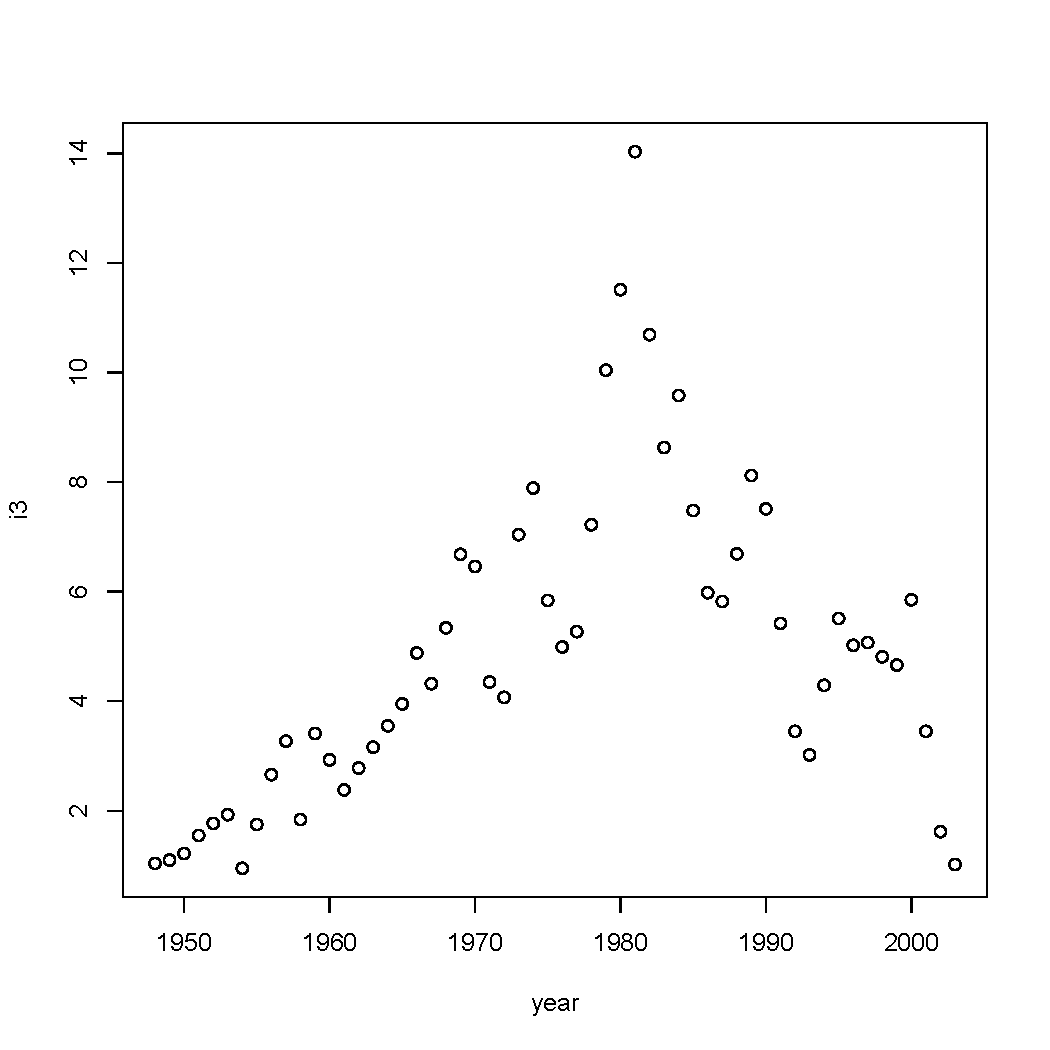
\includegraphics[scale=.5]{intdef}
  \caption{Interest Rate Time Series Plot in R}
  \label{figure:intdef}
\end{figure}

For a simple side-by-side comparison of some basic functions of both MATLAB and R, see Table~\ref{tab:matlab-r-funcs}.
\begin{table}[htbp]
	\centering
	\begin{tabular}{lll}
	\toprule
	Function & MATLAB & R \\
	\hline
	Expansion & Toolboxes & Packages \\
	Programming & M code & R code \\
	File Input & \texttt{load} & \texttt{read.table} \\
	Getting Help & \texttt{help plot} & \texttt{?plot} \\
	Matrices & rows, then columns & columns, then rows \\
	Change Directory & \texttt{cd(`/path')} & \texttt{setwd(`/path')} \\
	\bottomrule
	\end{tabular}
	\caption{Basic Functions in MATLAB and R}
	\label{tab:matlab-r-funcs}
\end{table}

\subsection{Loading Data}
\paragraph{MATLAB.} There are a few ways to load data. The easiest is \texttt{load}\index{load@\texttt{load} (in MATLAB)}. To create an array variable name \texttt{plainTS} from a single-column text file \texttt{plain.txt}, we need the statement,
\ecaption{Loading single-column text file in MATLAB}
\begin{verbatim}
plainTS=load(`/path/plain.txt');
\end{verbatim}

The semicolon at the end of the statement suppresses any output to the screen. Leaving out the semicolon would display each line of text as it read into MATLAB. If our data set had multiple columns which were separated by spaces or tabs, we could use the same syntax, and we would still have a single variable, but with multiple columns. To refer to a single item in the array, such as the 27th observation, we address it \texttt{plainTS(27)}. If we had multiple columns, we want to refer to column 2, we simply use \texttt{plainTS(:,2)}.

Importing delimited data sets requires \texttt{dlmread}\index{dlmread@\texttt{dlmread} (in MATLAB)}, and is not much more difficult. To read only the numerical data from the five-column  tab-delimited file, \texttt{SP-MidCap4.txt}
\ecaption{Loading multiple-column tab-delimited text file in MATLAB}
\begin{verbatim}
sp_mid=dlmread(`/path/SP-MidCap4.txt', `\t', 0, 1);
\end{verbatim}
The \texttt{`\textbackslash t'} is the delimiter, which in our case is the tab character. To use comma-delimited text, we replace that with `,' or whichever marker we require. We can specify the starting column and row number of the data. MATLAB uses a zero-based index, so to get \emph{all rows} but columns 1 to whichever is the last column, we enter 0 and 1, respectively. Once loaded, we have a variable named \texttt{sp\_mid}. To refer to the 120th row, and 3rd column data item, \texttt{sp\_mid(120,3)}.

Now try to load \texttt{SP-MidCap.csv} which is comma-delimited and has the first row consisting of column names. We do not want to import the first column, which are non-numerical dates, nor do we want the column names, since they too are non-numerical.
\ecaption{Loading multiple-column comma-delimited text file in MATLAB}
\begin{verbatim}
sp_mid=dlmread(`/path/SP-MidCap.csv', `,', 1, 1);
\end{verbatim}

There are other methods in MATLAB for loading data and writing results back to a file, but these two will work fine for most purposes. We have also only concerned ourselves with numerical data at this point. We address date conversions in Section~\ref{date-handling}.

\paragraph{R Environment.} Just as we explored one method of loading tab-delimited data and one method for comma-delimited data in MATLAB, we will discuss two ways in the R environment. One advantage is that we may load column names with our data, something we are unable to do in MATLAB. We will load all data, \emph{including column names}, from the five-column  tab-delimited file, \texttt{SP-MidCap3.txt} using \texttt{read.table}.\index{read.table@\texttt{read.table} (in R)}
\ecaption{Loading multiple-column tab-delimited text file in R}
\begin{verbatim}
mid400<-read.table(`/path/SP-MidCap3.txt', header=T)
\end{verbatim}

\pagebreak
We have two ways of using the column names from a data set. The first method is easier, but can result in name collision when multiple data sets are loaded.
\marginpar{\begin{small}\begin{flushleft}\textcolor{blue}{Name collision is the result of two processes or data sets using the same name.}\end{flushleft}\end{small}}
Now that we have \texttt{SP-MidCap3.txt} stored into a variable named \texttt{mid400}, we can assign columnn names using \texttt{attach(mid400)}\index{attach@\texttt{attach} (in R)}.
To see the names assigned to columns, we can use \texttt{names(mid400)}\index{names@\texttt{names} (in R)}.

We can refer directly to the column of data by its name, such as when we want the mean of the column \texttt{Close}, by typing \texttt{mean(Close)}. The problem is that these column names are global, which is generally a bad idea in the event that we want other data with the same name.

The second method of using the column names from a data set is preferred, and is only slightly more complex.  We do not use the \texttt{attach} statement, but instead refer to a column by variable name and column name using \texttt{with}\index{with@\texttt{with} (in R)}. We can compute the mean of the column \texttt{Close}, by typing \texttt{with(mid400, mean(Close))}.
We still have the column names in the variable, and we can view the first row of data by typing \texttt{mid400[1,]}.

Reading comma-separated data is as easy as reading table data -- the tab or space delimited files we just discussed. This time, we use the statement, 
\texttt{read.csv}\index{read.csv@\texttt{read.csv} (in R)}.
\ecaption{Loading multiple-column comma-delimited text file in R}
\begin{verbatim}
mid400<-read.csv(`/path/SP-MidCap.csv', header=T)
\end{verbatim}
Once the data set is loaded, all functions work exactly the same as before.

\subsection{Date Handling}\label{date-handling}\index{Epoch Date}
\paragraph{Date Formatting.} Most computer systems store a date as the number of days or number of minutes since a specific date.
\marginpar{\begin{small}\begin{flushleft}\textcolor{red}{Be aware of the computer epoch date of the system you import and export into.}\end{flushleft}\end{small}}
Some Unix systems store the date as number of days since January 1, 1970, while some software may use a different date. This ``epoch date'' may cause confusion when reading and writing dates into a statistical package. For instance, what is the date value of 733671? That depends on which system created that date. This particular date value came from MATLAB, where it represents September 20, 2008, but in Excel (with 1904 Date System enabled) it is September 21, 3912, and it is September 20, 3908 with 1904 Date System disabled.

The spreadsheet software in OpenOffice for X11 uses a date value of 1 for December 31, 1899 (\emph{which is technically January 0, 1900}), but Microsoft Excel uses January 1, 1904, the Lotus 1-2-3 ``standard.'' In Excel, the ``1904 Date System'' can be turned off, so that date value of 1 becomes January 1, 1900.

\paragraph{MATLAB.} Dates must be stored as numbers in MATLAB, which measures the number of days since January 1, 0. There are functions to convert a string date into a number. For example the date, 20 September 2008, could be entered a few ways, such as,
\index{datenum@\texttt{datenum} (in MATLAB)}
\begin{verbatim}
my_date=datenum(`2008-09-20', `yyyy-mm-dd')
my_date=datenum(`20-Sep-2008')
\end{verbatim}
which stores the number 733671 in the variable \texttt{my\_date}. This makes date arithmetic easier, but, that number does not tell us much once stored since we like seeing months, days, and years. We can convert that number to a date string using \texttt{datestr(my\_date)}.\index{datestr@\texttt{datestr} (in MATLAB)} If we want the month, day, and year as a number, we have \texttt{[yr,mo,day]=datevec(my\_date)}\index{datevec@\texttt{datevec} (in MATLAB)}, which populated three variables as described in the left-hand side.

\paragraph{R Environment.} Our data set \texttt{mid400} has a column named \texttt{Date} which is formatted \texttt{yyyy-mm-dd}. This works well for date conversion and performing date arithmetic. To convert the item into a ``time'' data type, we need \texttt{as.POSIXlt}\index{as.POSIXlt@\texttt{as.POSIXlt} (in R)} 
so that converting the date in column 1, row 1 is done by \texttt{as.POSIXlt(mid400[1,1])}. To add 7 days to that date is as easy as \texttt{as.POSIXlt(mid400[1,1]) + (24*60*60*7)}.

R also has a full set of objects that can display and manipulate dates.
\begin{verbatim}
today<-Sys.Date()
next.week<-today+7
format(next.week, "%d %b %Y")
\end{verbatim}

\subsection{Statistical Operations}
\paragraph{MATLAB.}
There is a wide variety of statistical functions available in MATLAB. As a very brief introduction, we will look at some basic descriptive statistics. Using our \texttt{sp\_mid} data set, we compute the mean and standard deviation of the set, using \texttt{mean} and \texttt{std}, respectively. We can summarize the entire data set, column-by-column with \texttt{mean(sp\_mid)}, which returns a matrix that has one row, and has a mean for each column.

If, for example, we want the standard deviation of the most recent 200 opening prices (column 1 of the data), we need to specify the range using \texttt{std(sp\_mid(1:200, 1))}.

\paragraph{R Environment.}
There is also an extensive variety of statistical functions available in R. As a very brief introduction, we will look at some basic descriptive statistics. Using our \texttt{mid400} data set, we compute the mean and standard deviation of the set, using \texttt{mean} and \texttt{sd}, respectively. We can summarize the entire data set, column-by-column with \texttt{mean(mid400)}, which returns the mean for each column, except for \texttt{Date}, which is not numeric.

If, for example, we want the standard deviation of the most recent 200 opening prices (column 2 of the data), we need to specify the range using \texttt{sd(mid400[1:200, 2])}.

\subsection{Functions}
\paragraph{MATLAB.} Sometimes, the built-in functionality of MATLAB is not enough to handle specific requirements. In order to extend the environment, users may write functions. Here is an example of a simple moving average.
\ecaption{Moving Average Function in MATLAB}
\begin{verbatim}
function y = movavg(x,p)
% Simple Moving Average written as a MATLAB demo
% by Andrew P. Acosta
% This works with a COLUMN of numbers only.
y=zeros(size(x));
for n=p:size(x,1)
    y(n)=mean(x(n-p+1:n));
end
\end{verbatim}

The elements of a function are the word \texttt{function} as the first keyword, followed by the variable(s) returned by the function. A MATLAB function can return more than one variable, provided that the list is enclosed in brackets (\textit{e.g.} \texttt{[x,y,z]}). Comments in MATLAB begin with a percent sign (\texttt{\%}). The contents of the comments placed between the first line of the function and the first line of instructions will display when a user types \texttt{help} followed by the function name. It is a good way of documenting user-defined code.

What follows is the actual work of the function. The return variable(s) must be set somewhere in this segment. The three-day moving average for the first ten observations is called by, \texttt{movavg(sp\_mid(1:10,1), 3)}.


\paragraph{R Environment.} Since R also is a programming language, there is a specific syntax for writing functions. Here is an example of a simple moving average.
\ecaption{Moving Average Function in R}
\begin{verbatim}
movavg<-function(x,p) { 
    # Simple Moving Average written as an R demo 
    # by Andrew P. Acosta
    y<-numeric(length(x))
    for(n in p:length(x)) {
        y[n]<-mean(x[(n-p+1):n])
        }
    y
}
\end{verbatim}

The elements of a function are the word \texttt{function} after assignment to the return variable. Comments in R begin with a pound or hash symbol sign (\texttt{\#}). 

What follows is the actual work of the function. The return variable must be set somewhere in this segment. The three-day moving average for the first ten observations is called by, \texttt{movavg(mid400[1:10,2], 3)}.

\subsection{Graphing}
\begin{figure}[tbh]
  \centering
  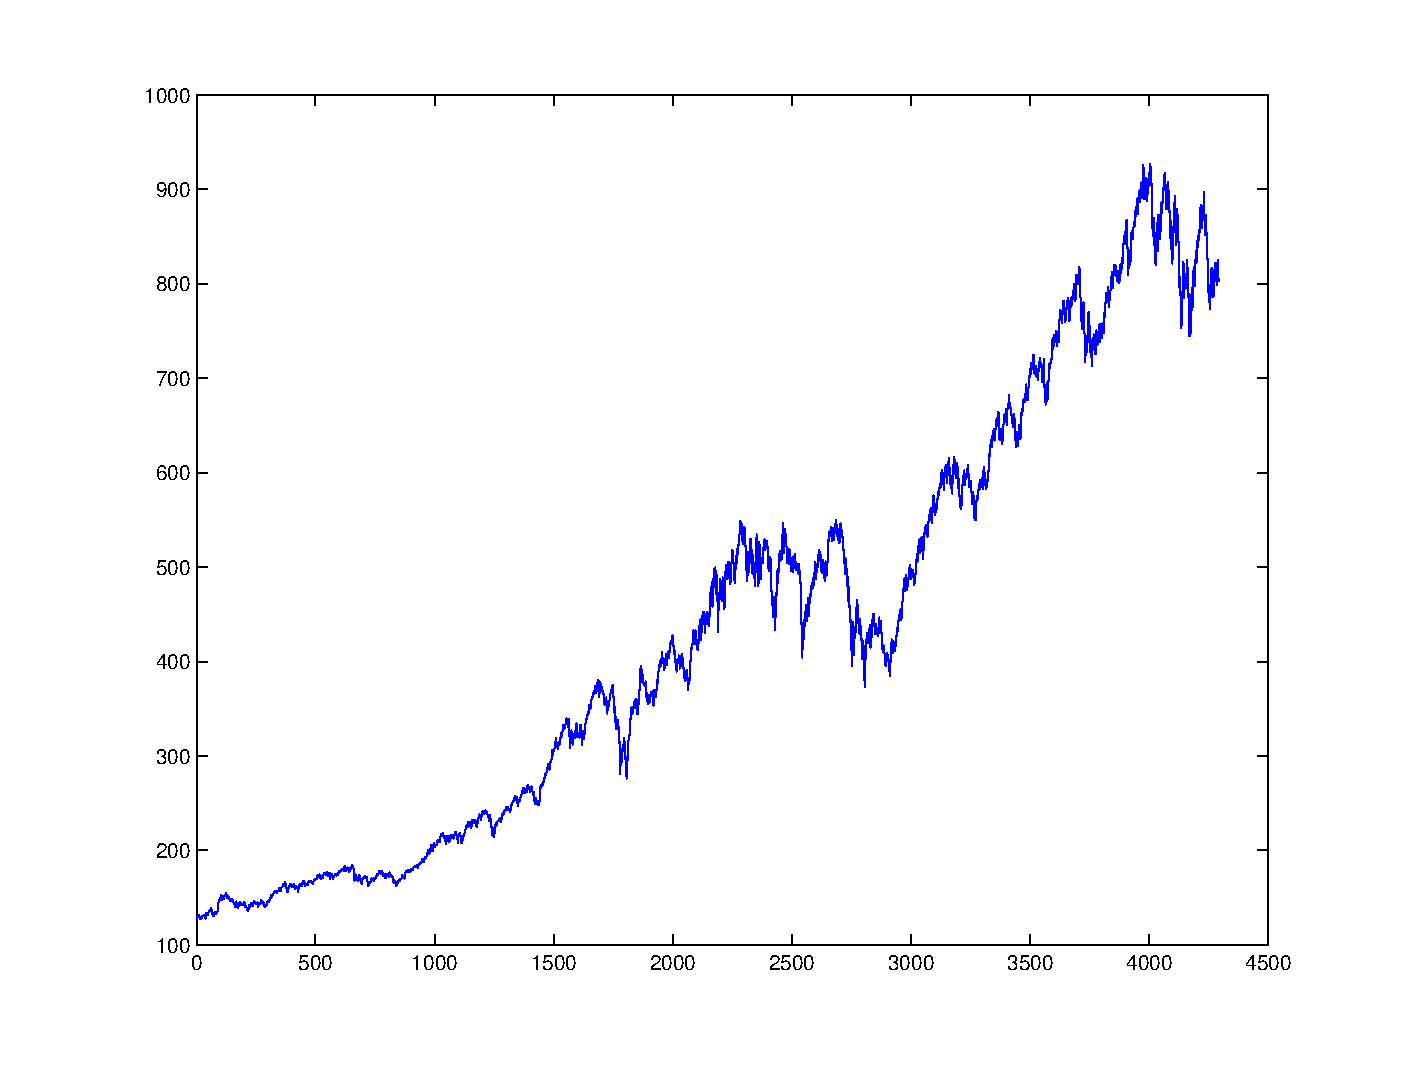
\includegraphics[scale=.5]{sp_mid}
  \caption[\texttt{SP-MidCap-sort.csv} Data Set in MATLAB]{Plot of \texttt{SP-MidCap-sort.csv} Data Set using MATLAB statement \texttt{plot(sp\_mid(:,1))}.}
  \label{figure:spmid}
\end{figure}
\paragraph{MATLAB.} There is an extensive collection of graphical features in MATLAB.  One of the most used functions is \texttt{plot}\index{plot@\texttt{plot} (in MATLAB)}, which creates an X,Y plot which is depicted in Figure~\ref{figure:spmid}.

To work with the data set as a MATLAB time series, we will explore the \texttt{timeseries}\index{timeseries@\texttt{timeseries} (in MATLAB)} and \texttt{tscollection}\index{tscollection@\texttt{tscollection} (in MATLAB)} objects. 

\paragraph{R Environment.} It is no surprise that R also has an extensive collection of graphical feaures.  One of the most used functions is \texttt{plot}\index{plot@\texttt{plot} (in R)}, which creates an X,Y plot which is depicted in Figure~\ref{figure:mid400}.
\begin{figure}[tbh]
  \centering
  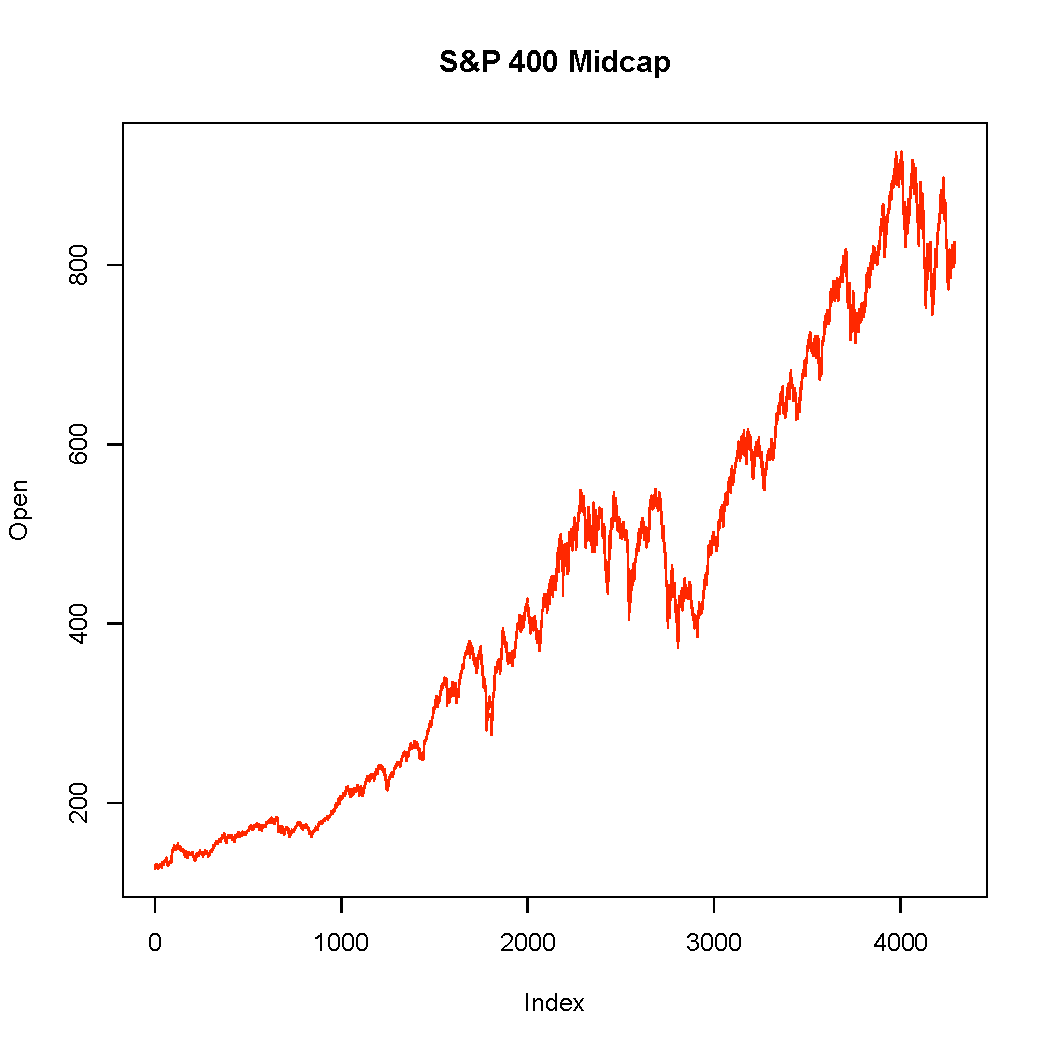
\includegraphics[scale=.6]{mid400}
  \caption[\texttt{SP-MidCap-sort.csv} Data Set in R]{Plot of \texttt{SP-MidCap-sort.csv} Data Set using R programming. \linebreak \texttt{with(mid400, plot(Open, type="l", col="red", ylab="Open", main="S\&P 400 Midcap"))}.}
  \label{figure:mid400}
\end{figure}

To work with the data set as an R time series, we will explore the \texttt{ts}\index{ts@\texttt{ts} (in R)} object. 

\pagebreak
\subsection{Technical Issues}
As with any data, there could be some level of work required to ``clean'' the data, or to make it presentable for analysis.  This cleanup effort will depend greatly upon the quality and source of the data, as well as the type of analysis and software.

Some issues arise at the source of \fts{} data, and generally become typical problems solved through information technology. Often, they are simple matters of parsing a text file, rearranging rows and columns, or validating source data. Such rudimentary tasks, as well as more complex pre-analytical text formatting, are solved by scripting languages like Perl\index{Perl Language} or Python\index{Python Language}.

Be aware that some \fts{} data may have the most recent data first, yet your graphics and numerical analysis expects oldest data first. In this case, you simply need to reverse the order of the observations in the data set.

Some data conversion is more complicated. For example, if a process is receiving XML\index{XML}-formatted data, it is worth knowing how the data are described by the format. The same applies to reading and writing HTML\index{HTML} data. MATLAB and R have capabilities of handling formatted data, but it is still important to know the underlying formatting issues.

In other cases, there may be missing data, or data that are simply incorrect. How would you react to a price series such as \{23.38, 26.73, \textbf{95.69}, 26.55, 26.47, 26.63\}? Do you explain the 95.69 that seems to be out of place? Does it belong there? Is it an error? How do you know? How do you locate these kinds of numbers in a large data set?

Even if the data is correct on some superficial level, there remain several other issues such as: of normalizing a variable's range, proper sampling methods, and capturing patterns. \citeA{pyle1999dpd} writes in detail about these concerns as well as many others.

No doubt, you will encounter errors in data, or require them to be modified in some way before or after your analysis. Being able to do this is vital, and the responsibility should not be relegated to a lesser importance.
\section{Applications of Financial Time Series}
\paragraph{Primary Text Reading.} \citeA[chap. 1]{tsay2005aft}\index{Tsay, Ruey}

\subsection{Asset Returns Over Time}
Let $P_t$ be the price of an asset at time $t$, and we assume no dividends are paid, then the one-period simple gross return is,
\begin{equation}
1 + R_t = \frac{P_t}{P_{t-1}} \text{\quad which is \quad} P_t = P_{t-1}(1 + R_t).
\end{equation}
The one-period simple return is simply the difference in value between two observations divided by its initial value,
\begin{eqnarray}
R_t &=& \frac{P_t}{P_{t-1}} -1 \label{eq:1pd-ret} \\
&=& \frac{P_t - P_{t-1}}{P_{t-1}}. \notag
\end{eqnarray}
The multiperiod simple return takes into account a series of one-period simple returns, thus making it the product of all asset return observations,
\begin{eqnarray}
1+R_t[k] = \frac{P_t}{P_{t-k}} &=& \frac{P_t}{P_{t-1}} \times \frac{P_{t-1}}{P_{t-2}} \times \cdots \times \frac{P_{t-k+1}}{P_{t-k}} \label{eq:multiperiod} \\
&=& (1+R_t)(1+R_{t-1})\cdots(1+R_{t-k+1}) \notag \\
&=& \prod^{k-1}_{j=0}(1+R_{t-j}). \notag
\end{eqnarray}
The $k$-period simple gross return is just the product of the $k$ one-period simple gross returns involved. This is a compound return. The $k$-period simple net return is $R_t[k]=(P_t - P_{t-k})/P_{t-k}$.

\begin{table}[htbp]
   \centering
   \begin{tabular}{rr}
      \toprule
      Day & Price \\
      \hline
      1 & 37.84 \\
      2 & 38.49 \\
      3 & 37.12 \\
      4 & 37.60 \\
      5 & 36.30 \\
      \bottomrule
   \end{tabular}
   \caption{Simple Return Closing Prices}
   \label{tab:simp-rets}
\end{table}

Using Table~\ref{tab:simp-rets}, what is the simple return from day 1 to day 2? 
\[
R_2 = \frac{38.49-37.84}{37.84} = 0.017.
\]

What is the simple return from day 1 to day 5? 
\[
R_5(4) = \frac{36.30-37.84}{37.84} = -0.041.
\]

\paragraph{Continuous Compounding.}
Extending \eqref{eq:1pd-ret}, if we can continually reduce the number of compounding periods, we have a continuous function of $e$,
\begin{equation}
A = C e^{r \times n}.
\end{equation}
For example, let us take a currency amount, $C=100$ at a continuously compounded rate, $r=.05$ for 3 years, $n=3$.
\[
A = 100 \exp(.05 \times 3) = 116.1834
\]
If we take the basic function for interest payment for rate $r$ and compound to $n$ periods per year, we have,
\[
\left(1+\frac{r}{n}\right)^n.
\]
For a single interest payment in year, $n=1$. Two payments per year, $n=2$, \textit{etc.} As we increase the compounding frequency $n$, we approach a limit.
\begin{eqnarray*}
1.05 &=&\left(1+\frac{.05}{1}\right)^1 \\
1.05063 &=&\left(1+\frac{.05}{2}\right)^2 \\
1.05095 &=&\left(1+\frac{.05}{4}\right)^4 \\
1.05116 &=&\left(1+\frac{.05}{12}\right)^{12} \\
1.05127 &=&\left(1+\frac{.05}{365}\right)^{365} \\
\\
1.05127 &=& \exp(.05)
\end{eqnarray*}

\begin{proof}
Increase the frequency of compounding $n$ while applying $1 + \frac{1}{n}$.
\[
e= \lim_{n \to \infty}\left (1+ \frac{1}{n} \right )^n
\]
\end{proof}

\paragraph{Continuously Compounded Returns.} The logarithm of the simple gross return of an asset is the continuously compounded return, also known as the \emph{log return},
\begin{equation}
r_t = \ln(1 + R_t ) = \ln \frac{P_t}{P_t-1}= p_t - p_t-1, 
\label{eq:log-return}
\end{equation}
where $p_t = \ln(P_t)$.

\paragraph{Multiperiod Log Returns.} The sum of continuously compounded one-period returns is the multiperiod return.
\begin{eqnarray*}
r_t(k) &=& \ln[1 + R_t (k)] \\
&=& \ln[(1 + R_t )(1 + R_{t-1}) \cdots (1 + R_{t-k+1})] \\
&=& \ln(1 + R_t ) + \ln(1 + R_{t-1}) + \cdots + \ln(1 + R_{t-k+1}) \\
&=& r_t + r_{t-1} + \cdots + r_{t-k+1}.
\end{eqnarray*}

\paragraph{Examples.} What is the \emph{log return} from day 1 to day 2? 
\[
r_2 = \ln(38.49) - \ln(37.84) = 0.017.
\]

What is the \emph{log return} from day 1 to day 5? 
\[
r_5(4) = \ln(36.3) - \ln(37.84) = -0.042.
\]

\subsection{Moments of Random Variables}\index{moment, (random variable)}
The $\ell$th moment of a continuous random variable $X$ is defined as
\begin{equation}
m^{'}_{\ell}=E(X^{\ell})=\int^{\infty}_{-\infty} x^{\ell}f(x)dx
\end{equation}
where $E$ is the expectation and $f(x)$ is the probability density function of $X$. The first moment is called the \emph{mean} or \emph{expectation} of $X$. It measures the central location of the distribution. We denote the mean of $X$ by $\mu_x$. The $\ell$th central moment of $X$ is
\begin{equation}
m_{\ell}=E[(X-\mu_x)^{\ell}] = \int^{\infty}_{-\infty} (x-\mu_x)^{\ell}f(x)dx
\end{equation}
\citeA[p. 8]{tsay2005aft}. With a random variable $X=\{x_1, \ldots, x_T\}$ of $T$ observations, we can compute the sample mean,
\begin{equation}
\hat{\mu_x}=\frac{1}{T} \sum^{T}_{t=1}x_t
\end{equation}
sample variance,
\begin{equation}
\hat{\sigma}^{2}_{x}=\frac{1}{T-1} \sum^{T}_{t=1}(x_t-\hat{\mu}_x)^2
\end{equation}
sample skewness,
\begin{equation}
\hat{S}(x)=\frac{1}{(T-1)\hat{\sigma}^3_x} \sum^{T}_{t=1}(x_t-\hat{\mu}_x)^3
\end{equation}
sample kurtosis,
\begin{equation}
\hat{K}(x)=\frac{1}{(T-1)\hat{\sigma}^4_x} \sum^{T}_{t=1}(x_t-\hat{\mu}_x)^4.
\end{equation}

Mean and variance of returns are important because they communicate long-term return and risk, respectively. The symmetry of the distribution has important implications in holding short or long financial positions and in risk management. Skew and kurtosis are important to volatility forecasting, efficiency in estimation and tests. 

\paragraph{Examining Distribution of Returns.} Using R, we load in the data set and examine column 2, which is the IBM returns data. To compare the returns to a normal distribution, we look at Figure~\ref{figure:ibm-qq}. The returns plotted over time are depicted in Figure~\ref{figure:ibm-ret}.
\begin{figure}[tb]
  \centering
  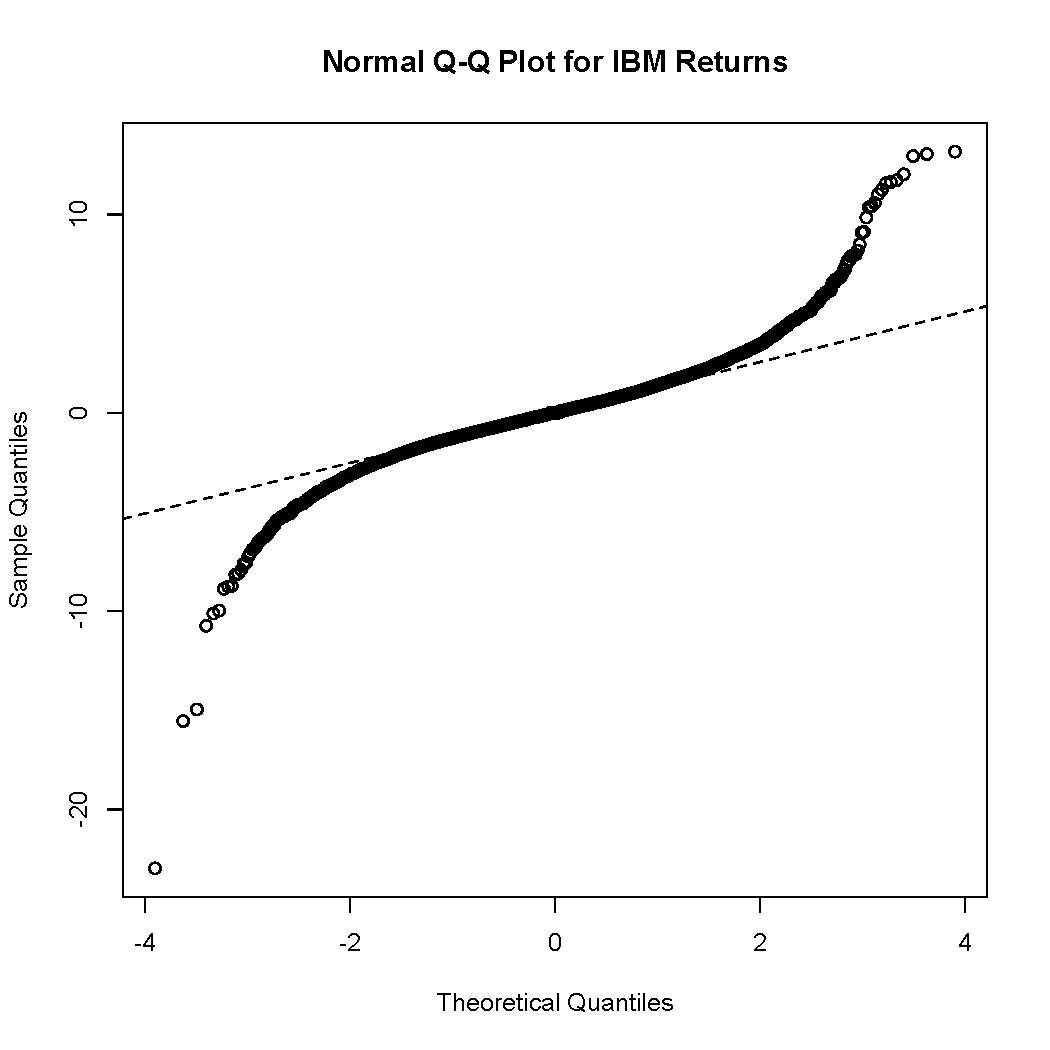
\includegraphics[scale=.5]{ibm-qq}
  \caption[Q-Q Plot of Returns]{By looking at a quantile-quantile plot of our data set, we see that returns are not normally distributed. The tails deviate sharply from normality.}
  \label{figure:ibm-qq}
\end{figure}

\index{R language} 
\begin{verbatim}
rets<-read.table("d-ibmvwewsp6203")
attach(rets)
retsts<-ts(V2,start=c(1962,190),frequency=260)
plot(retsts,ylab="IBM Returns", typ="p") 

qqnorm(V2,main="Normal Q-Q Plot for IBM Returns")
qqline(V2,lty=2)
\end{verbatim}

\begin{figure}[tb]
  \centering
  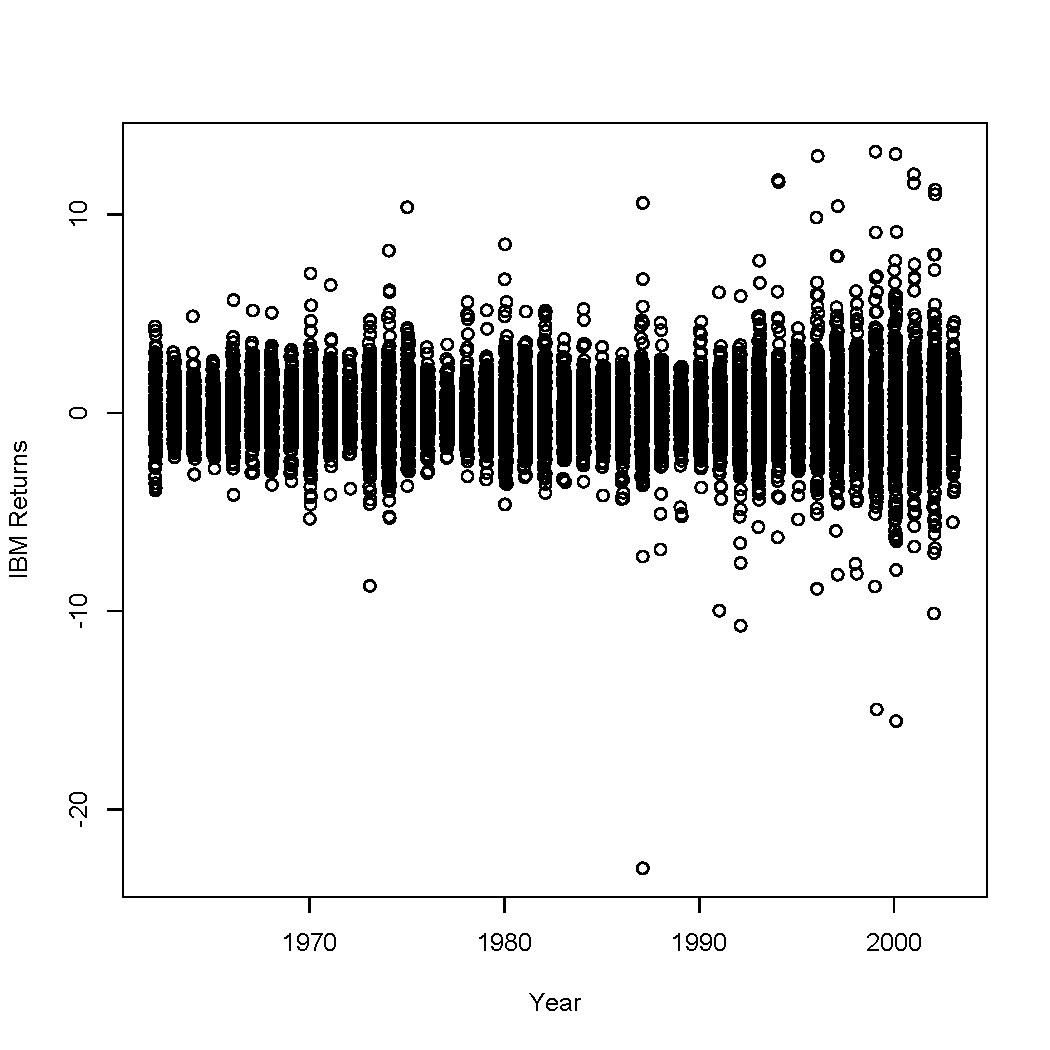
\includegraphics[scale=.5]{ibm-ret}
  \caption[IBM Returns]{IBM returns become more varied over time, deviating further from zero.}
  \label{figure:ibm-ret}
\end{figure}

\paragraph{Normal Distribution.} For the sake of simplicity, returns are often considered to be \emph{\mbox{normally} distributed}. However, the lower bound of a simple is -1, total loss of the asset. The normal distribution has no lower bound. Also, multiperiod returns (\emph{the product of one-period \mbox{returns}, \eqref{eq:multiperiod} is a multiperiod return}) of a normally distributed returns are themselves not normally distributed. Additionally, asset returns observed in reality have positive excess kurtosis, and do not fit the normal distribution.

\paragraph{Lognormal Distribution.} Instead of assuming a normal distribution, we could assume that the log returns $r_t$ of an asset are independent and identically distributed (\emph{iid})\index{iid -- independent and\\identically distributed} as normal with mean $\mu$ and variance $\sigma^2$, which makes simple returns iid\index{iid -- independent and\\identically distributed} lognormal random variables, and mean and variance are,
\[
E(R_t)=\exp \left( \mu + \frac{\sigma^2}{2} \right) -1, \quad
\text{Var}(R_t) = \exp(2\mu+\sigma^2)[\exp(\sigma^2)-1].
\]
The mean and variance of the log returns $r_t$ when $m_1$ and $m_2$ are the mean and variance of the simple return $R_t$
\[
E(r_t) = \ln \left( \frac{m_1+1}{\sqrt{1+m_2 / (1+m_1)^2}} \right), \quad
\text{Var}(r_t)=\ln \left( 1+\frac{m_2}{(1+m_1)^2} \right).
\]
$Y$ is lognormal if $X = \ln(Y)$ is normal.

\subsection{Power Generation and Delivery Time Series}
As a practical example of \fts{}, we will briefly focus on power generation and delivery -- the route that electricity makes in its supply chain from fuel to its consumption in homes and businesses. Electricity demand is contingent upon weather, among other factors. Likewise, the supply of electricity requires consideration of many time series.

Some background reading to understand the power generation and delivery fundamentals are at the EIA website., ``How is my electricity generated, delivered, and priced?''\footnote{The U.S. Energy Information Administration publishes detailed statistics and news regarding energy production and consumption on it web site \texttt{http://www.eia.doe.gov}. A good introduction to electricity generation is at  \texttt{http://tonto.eia.doe.gov/energy\_in\_brief/electricity.cfm}}.

\paragraph{Generation.} When considering how electricity is generated, we must consider sources of generation,
\begin{enumerate}
	\item coal
	\item natural gas
	\item nuclear
	\item hydroelectric
	\item wind
	\item others \ldots
\end{enumerate}
Some of these source require a fuel source to create heat, which boils water to create steam to turn electricity-generating turbines. Clearly, our analysis of \fts{} should include inputs like fuel costs.

Power plants cannot operate every minute of every day. There will be times that require maintenance or refueling. The time to perform these tasks might be several weeks, and some outages are planned, others are unplanned. For this reason, multiple power stations will be generating concurrently. This is also a factor that must considered when modeling the generation of power.

\paragraph{Delivery.} Electricity, when generated at a power plant, must be transmitted distances to areas for local consumption. There is only so much power that can travel across high-voltage lines at any given time. When demand is very high, the transmission lines reach a point of \emph{congestion}. When this occurs, the best route through which to deliver power must be obtained very quickly.

\subsubsection{Weather}
Performing quantitative weather prediction uses current weather conditions as an input into mathematical models of the atmosphere to predict temperature and rainfall.
\margincomment{Computer models forecast changes in temperature and rainfall.}
These predictions are important to power generation and delivery because electricity demand has some relationship to the current temperature. Power sources such as hydroelectric and wind require plenty of upstream water and winds to produce electricity.

Due to the complex nature of weather modeling, it is only feasible to create any reliable and timely forecasts in real-time with advanced computing technology. The task requires manipulating very large datasets and performing complex calculations. Using \emph{ensemble forecasts}\index{ensemble forecasts} helps us to define the forecast uncertainty and extend weather forecasting farther into the future than would otherwise be possible.

A model, in this context, is a computer program that produces meteorological information for future times at given positions and altitudes. The horizontal domain of a model is either global, covering the entire Earth, or regional, covering only part of the Earth. Regional models also are known as limited-area models.

The forecasts are computed using mathematical equations for the physics and dynamics of the atmosphere. These equations are \emph{nonlinear} and are impossible to solve exactly.
\margincomment{Numerical forecast methods obtain approximate solutions.} Different models use different solution methods. Global models often use \emph{spectral methods}\index{spectral methods} for the horizontal dimensions and finite difference methods for the vertical dimension, while regional models usually use finite-difference methods in all three dimensions. Regional models also can use finer grids to explicitly resolve smaller-scale meteorological phenomena, since they do not have to solve equations for the whole globe. We discuss examples of spectral methods in Section~\ref{spectral methods}.

Models are initialized using observed data from weather satellites and surface weather observation stations. The irregularly-spaced observations are processed by data assimilation and objective analysis methods, which perform quality control and obtain values at locations usable by the model's mathematical algorithms (usually an evenly-spaced grid). The data are then used in the model as the starting point for a forecast. Commonly, the set of equations used is known as the \emph{primitive equations}. These equations are initialized from the analysis data and rates of change are determined. The rates of change predict the state of the atmosphere a short time into the future.

The equations are then applied to this new atmospheric state to find new rates of change, and these new rates of change predict the atmosphere at a yet further time into the future.
\margincomment[red]{Most time series analysis assumes evenly-spaced observations. We cannot make that assumption in weather modeling.}
This time stepping procedure is continually repeated until the solution reaches the desired forecast time. The length of the time step is related to the distance between the points on the computational grid. Time steps for global climate models may be on the order of tens of minutes, while time steps for regional models may be a few seconds to a few minutes.

\paragraph{Ensemble Forecasts.} Long-range weather forecasting requires the application of some theory taken from fluid dynamics \cite{lorenz1969pfp}. Ensembles were proposed by Edward Lorenz\index{Lorenz, Edward} in an attempt to make extended forecasts despite the chaotic nature of the fluid dynamics equations required. There is tremendous amounts of uncertainty during the path of a weather pattern, which covers thousands of miles. To account for this uncertainty, stochastic or ``ensemble" forecasting is used, involving multiple forecasts created with different model systems, different physical parametrizations, or varying initial conditions. The ensemble forecast is usually evaluated in terms of the ensemble mean of a forecast variable, and the ensemble spread, which represents the degree of agreement between various forecasts in the ensemble system, known as ensemble members.

\subsubsection{Fuel Prices}
In most cases, to generate electricity at a power plant, we require a fuel of some kind. That fuel may be coal, natural gas, or nuclear fuel such as uranium. The price to purchase and receive for delivery these fuels is affected by market forces.

\paragraph{Natural Gas.}
One of the most abundant fuel sources for power generation is natural gas. The contracts for delivery have different terms, and delivery points throughout North America \cite[p.3--5]{eydeland-wolyniec2002}.
\begin{itemize}
	\item\index{natural gas delivery!baseload firm}\index{baseload firm|see{natural gas delivery}}{\textbf{Baseload Firm}. In this transaction, the delivering party is expected to perform according to the contract under most any conditions.}
	\item\index{natural gas delivery!baseload interruptible}\index{baseload interruptible|see{natural gas delivery}}{\textbf{Baseload Interruptible}. Delivery can be interrupted, and the conditions may or may not be specific in the contract.}
	\item\index{natural gas delivery!swing}\index{swing|see{natural gas delivery}}{\textbf{Swing}. The volume of delivered gas is adjusted daily at the buyer's discretion, typically for daily pipeline volume balancing.}
\end{itemize}

\paragraph{Transportation.}
Contractual provisions of natural gas delivery may vary.
\begin{itemize}
	\item\index{natural gas transportation!firm transportation service}{\textbf{Firm Transportation Service}. Firm transportation service is the highest priority service.}
	\item\index{natural gas transportation!interruptible transportation contract}{\textbf{Interruptible Transportation Contract}. A pipeline has an option to interrupt the service on short notice without a penalty.}
\end{itemize}

\subsubsection{Electricity Delivery Capacity}
\paragraph{Energy Markets.}
In order to coordinate delivery across state boundaries and to ensure competitive power markets, there are independent system operators\index{independent system operator} (``ISO") and regional transmission organizations\index{regional transmission organization} (``RTO"). One example of an RTO is the \emph{PJM Interconnection} which has the task of coordinating the continuous buying, selling and delivery of wholesale electricity throughout the Pennsylvania, New Jersey, and Maryland area, as well as parts of Illinois, Indiana, Michigan. In its role as market operator, PJM balances the needs of suppliers, wholesale customers and other market participants and monitors market activities to ensure open, fair and equitable access.

PJM operates much like an exchange, with market participants establishing prices for electricity by matching supply and demand. The market uses \emph{locational marginal pricing}\index{locational marginal pricing} (LMP) that reflects the value of the energy at the specific location and time it is delivered. If the lowest-priced electricity can reach all locations, prices are the same across the entire grid. When there is transmission congestion, energy cannot flow freely to certain locations. In that case, more-expensive electricity is ordered to meet that demand. As a result, the locational marginal price is higher in those locations.

The energy market consists of \emph{day-ahead} and \emph{real-time} markets. The Day-Ahead Market is a forward market in which hourly LMPs are calculated for the next operating day based on generation offers, demand bids and scheduled bilateral transactions. The real-time Market is a spot market in which current LMPs are calculated at five-minute intervals based on actual grid operating conditions. Real-time prices are available. An RTO settles transactions hourly and issues invoices to market participants monthly.

\paragraph{Electricity Prices.} Electricity prices tend to experience abrupt price spikes\index{price spikes}, which are very short-term price increases of unpredictable magnitude \cite[p. 25]{weron2006mfel}\footnote{A good introduction to energy trading is \citeA{fusaro1998erm}. Although a bit dated by now, it contains some important fundamentals of the fuel markets. Further detail on price and volatility modeling can be found in \citeA{pilipovic2007er}.}.
\margincomment[red]{Electricity prices are extremely volatile, but follow a seasonal pattern.}
Because of these spikes, measuring the volatility of electricity prices is an important issue. Additionally, electricity demand tends to fluctuate seasonally, and we should expect its price to follow that pattern in some way.

Price volatility is not a single number, but rather, an array of numbers through time. How much fluctuation is observed in electricity prices to be delivered in ten minutes will not have the same fluctuation as that delivered in an hour, or a week from now. To represent this array, we require a \emph{term structure of volatility}\index{term structure of volatility} \cite[p. 328]{harris2006em},
\begin{equation}
\sigma_{a,T,t} = \Bigg( \frac{1}{(T-t)} \int^T_t \sigma^2(s)ds \Bigg)^{0.5}
\label{eq:tsov}
\end{equation}
where $T$ is the contract delivery date and $t$ is the observation date.

We shall see in Section~\ref{garch-spec} and in Section~\ref{crosscorrmatr} how to implement the term structure in \eqref{eq:tsov} to create volatility models. Using power generation and delivery as one example of a market with several kinds of \fts{}, we can further explore the numerical methods that give us insight into the markets themselves.
\section{Linear Time Series Analysis}
\paragraph{Primary Text Reading.} \citeA[chap. 2]{tsay2005aft}\index{Tsay, Ruey}

A collection of asset returns, such as the log returns of an asset \eqref{eq:log-return} is a \emph{linear time series}. Some of the elements of this analysis are: stationarity, dynamic dependence, autocorrelation function, modeling, and, forecasting. Models include:
\begin{enumerate}
\item simple autoregressive (AR)
\item simple moving average (MA)
\item mixed autoregressive moving-average (ARMA)
\item seasonal models
\item unit-root nonstationary
\item regression models with time series errors
%\item fractionally differenced models for long-range dependence
\end{enumerate}

\subsection{Stationarity}
Strict stationarity occurs when joint distributions $P(X \cap Y)$ are time-invariant, or in other words, $X:(r_{t_1}, \ldots, r_{t_k})$ is identical to $Y:(r_{t_{1+t}}, \ldots, r_{t_{k+t}})$ for all $t$. A weak stationarity exists if the mean of $r_t$ and the covariance between $r_t$ and $r_{t-\ell}$ are time-invariant, where $\ell$ is an arbitrary integer. What this means in practice is that asset values fluctuate with constant variation around a fixed level so that we can make inferences about future observations. The mean, or expectation, of returns is therefore $\mu = E(r_t)$ and the variance of returns is $\text{Var}(r_t) = E[(r_t - \mu)^2]$.

\subsection{Correlation and ACF}
The correlation coefficient between two random variables $X$ and $Y$ is
\[
\boxed{\quad \rho_{X,Y}={\mathrm{cov}(X,Y) \over \sigma_X \sigma_Y} ={E((X-\mu_X)(Y-\mu_Y)) \over \sigma_X\sigma_Y}, \quad}
\]
where $\mu_X$ and $\mu_Y$ are expected values of $X$ and $Y$ respectively, and $\sigma_X$ and $\sigma_Y$ are its standard deviations. Thus, the sample correlation is
\begin{eqnarray}
r_{xy}&=&\frac{\sum x_iy_i-n \bar{x} \bar{y}}{(n-1) s_x s_y} \\
\smallskip
&=&\frac{n\sum x_iy_i-\sum x_i\sum y_i} {\sqrt{n\sum x_i^2-(\sum x_i)^2}~\sqrt{n\sum y_i^2-(\sum y_i)^2}}. \notag
\end{eqnarray}

\paragraph{Autocorrelation Function (ACF).} When we want to examine the linear dependence between $r_t$ and its previous values $r_{t-\ell}$ we are interested in the lag-$\ell$ \emph{autocorrelation} of the series $r_t$.
\marginpar{\begin{small}\begin{flushleft}\textcolor{blue}{Existence of serial correlations implies that the return is predictable, indicating market inefficiency.}\end{flushleft}\end{small}}
The extent to which the series exhibits autocorrelation can help us determine how much of today's asset value has been determined by previous values. We could perform a hypothesis test for zero serial correlations, which would imply market efficiency,
\begin{eqnarray*}
H_0 : r_{XY} &=& 0 \\
H_a : r_{XY} &\ne& 0.
\end{eqnarray*}
Our null hypothesis $H_0$ is that this market is efficient, and our alternative hypothesis $H_a$ is that this market is \emph{not} efficient. Some sources of serial correlations found in \fts{} are,
\begin{itemize}
\item Nonsynchronous trading (Section~\ref{High-Frequency}) 
\item Bid-ask bounce (Section~\ref{High-Frequency}) 
\item Risk premium, \textit{etc}. (Section~\ref{Conditional Heteroskedastic})
\end{itemize}
Thus, significant sample ACF does not necessarily imply market 
inefficiency. 

\paragraph{Portmanteau test.} To look for autocorrelation, we will run a \emph{portmanteau test}\index{Portmanteau test}, which tests whether any of a group of autocorrelations of a time series are different from zero. Two portmanteau tests we will use are the Box-Pierce test and the Ljung-Box test. The Ljung-Box test can be defined as \\
$H_0$: 	The data are random. \\
$H_a$: 	The data are not random.
\bigskip

The Ljung-Box test statistic is calculated as
\begin{equation}
Q_{LB}=n(n+2)\sum_{k=1}^s r_k^2/(n-k).
\label{eq:Ljung-Box}
\end{equation}
where, \\
$n$ = number of observations \\
$s$ = number of coefficients to test autocorrelation \\
$r_k$ = autocorrelation coefficient (for lag $k$).
\bigskip

If the sample value of $Q_{LB}$ exceeds the critical value of a chi-square distribution with $s$ degrees of freedom, then at least one value of $r$ is statistically different from zero at the specified significance level. The null hypothesis is that none of the autocorrelation coefficients up to lag $s$ is different from zero.

We will use R to examine autocorrelation graphically, and then to perform a test for randomness, or lack of serial correlation of data.
\begin{verbatim}
rets<-read.table("aapl.txt")
s1<-acf(rets$Log.Return, lag=15, main="Autocorrelation of AAPL")
s1$acf
Box.test(rets, lag=15)
Box.test(rets, lag=15, type="Ljung")
\end{verbatim}

The dotted lines in Figure~\ref{figure:aapl-acf} represent the 95\% confidence interval of the ACF function. Notice that the vertical lines do not cross the dotted line boundary, which would indicate statistical significance from zero.

The first \texttt{Box.test} gives us the \emph{Box-Pierce test}\index{Box-Pierce test} of our log returns with $\chi$-squared = 14.7735, df = 15, $p$-value = 0.4679. The second \texttt{Box.test} gives us the \emph{Ljung-Box test}\index{Ljung-Box test}, $\chi$-squared = 15.0983, df = 15, $p$-value = 0.4444.

\begin{figure}[tb]
  \centering
  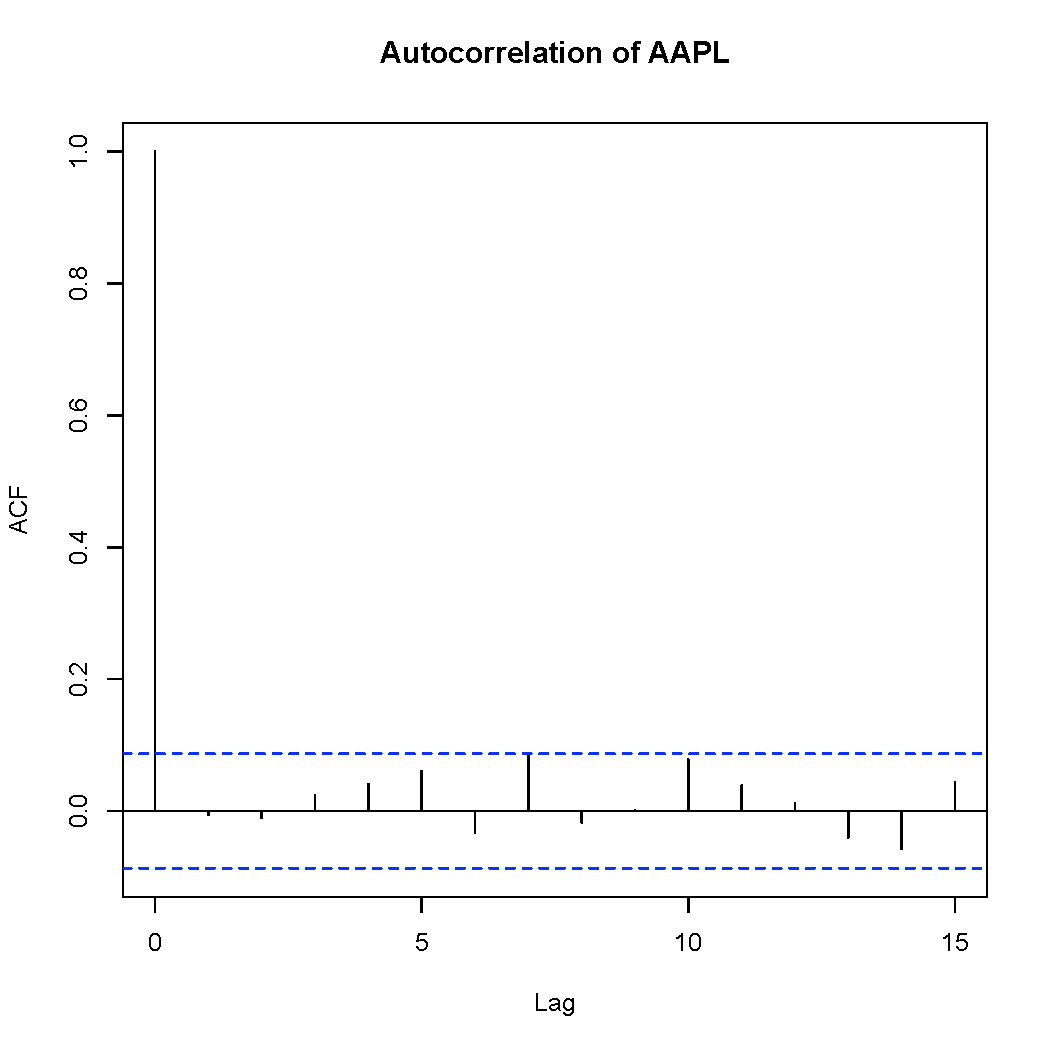
\includegraphics[scale=.6]{aapl-acf}
  \caption{ACF function of AAPL log returns with 15-day lag.}
  \label{figure:aapl-acf}
\end{figure}

Using R to generate the appropriate $\chi$-squared statistic to determine the critical region, \texttt{qchisq(p=0.4444, df=15)}, we get 13.60595. The hypothesis of randomness is rejected if $Q_{LB} > \chi^2(p, df)$. In this case, since our $p$-value is not more extreme than our $\alpha$ of 0.05, we do not reject the hypothesis that the data are random.

\pagebreak
\begin{figure}[tb]
  \centering
  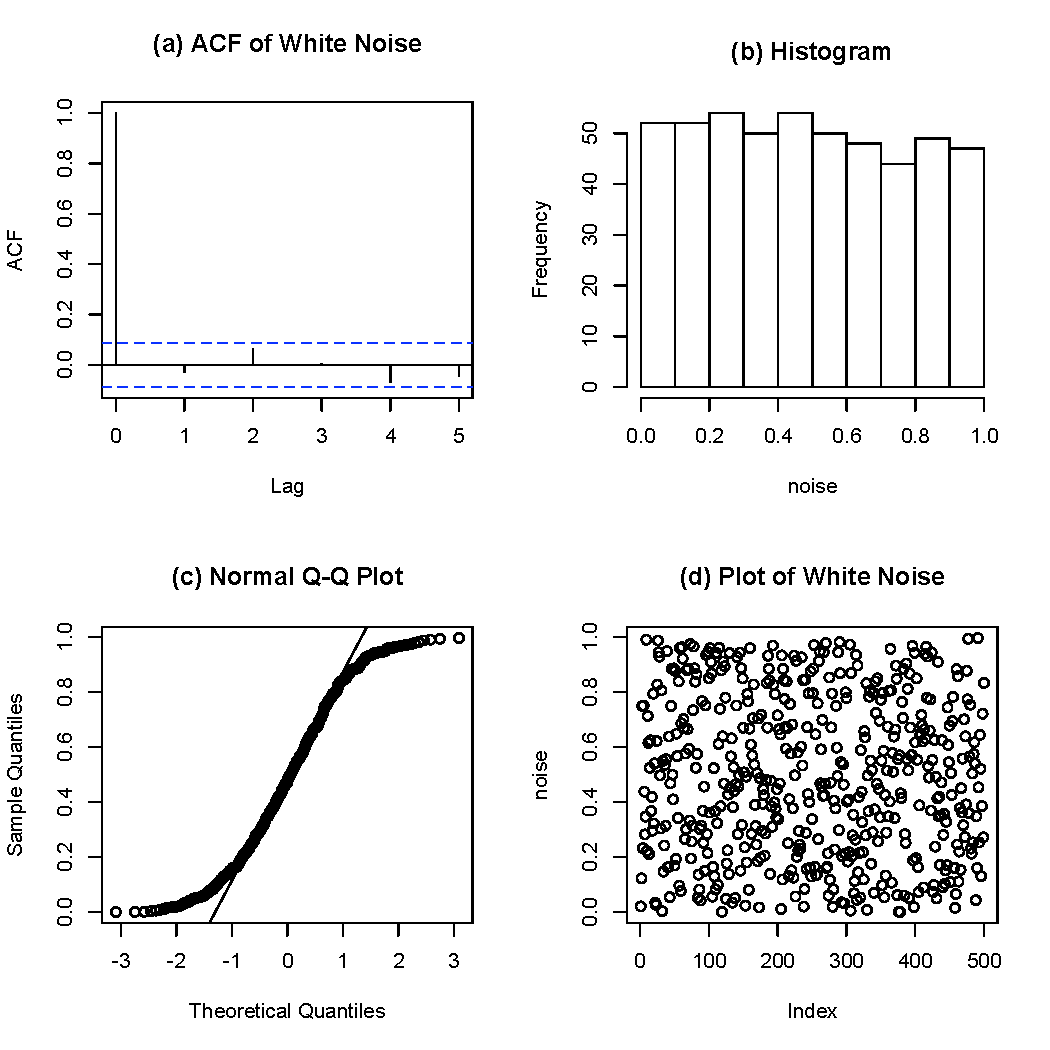
\includegraphics[scale=.7]{noise}
  \caption[Properties of White Noise]{White noise has an ACF of zero as seen in (a). We see in (b) a nearly uniform distribution, and in (c) we observe that the tails are not normally distributed. The values are plotted in (d).}
  \label{figure:noise}
\end{figure}

\paragraph{White Noise.}\index{White Noise}\index{Time Series!white noise} A time series $r_t$ that is a sequence of iid random variables with a finite mean and variance is \emph{white noise}. The serial correlation of any two points in $r_t$, regardless of lag, is zero, thus ACF values of white noise is zero. Using R to demonstrate, we can see the results in Figure~\ref{figure:noise}. In some circumstances, log returns of asset values can be considered white noise. With this assumption, we can create linear time series models.
\ecaption{White Noise in R}
\begin{verbatim}
noise=runif(5000) # Random numbers from Uniform Distribution
layout(rbind(c(1,2), c(3,4)))
acf(noise,lag=5, main="(a) ACF of White Noise")
hist(noise, main="(b) Histogram")
qqnorm(noise, main="(c) Normal Q-Q Plot")
qqline(noise)
plot(noise, main="(d) Plot of White Noise")
\end{verbatim}

Thus, we can implement a linear time series as
\begin{equation}
r_t = \mu + \sum^{\infty}_{i=0} \psi_i a_{t-i}
\end{equation}
where $\mu$ is the mean of $r_t$, $\psi_0=1$, and $\{a_t\}$ is a sequence of iid random variables.

\subsection{Simple Autoregressive Models}
Within a linear time series, there may exist a certain random movement, described as white noise $a_t$ with a mean of zero and variance of $\sigma^2_a$. This allows us to create a simple model
\begin{equation}
r_t = \phi_0 +\phi_1 r_{t-1} + a_t,
\label{eq:ar1}
\end{equation}
which follows the form of simple linear regression, where $r_t$ is the dependent variable, and $r_{t-1}$ is the independent variable. Equation~\eqref{eq:ar1} is the autoregressive (AR) model of order 1, also known as AR(1). We can generalize \eqref{eq:ar1} to the AR($p$) model
\begin{equation}
r_t = \phi_0 +\phi_1 r_{t-1} + \cdots + \phi_p r_{t-p} + a_t.
\label{eq:arp}
\end{equation}

\paragraph{AR Models.} We assume that \eqref{eq:ar1} has weak stationarity, and $E(r_t)=\mu$, $\text{Var}(r_t)=\gamma_0$, and $\text{Cov}(r_t,r_{t-j})=\gamma_j$, where $\mu$ and $\gamma_0$ are constant and $\gamma_j$ is a function of $j$, not $t$. This gives us a weakly stationary AR(1) model
\[
\text{Var}(r_t) = \gamma_0=\frac{\sigma^2}{1-\phi^2_1}, \text{ and \:} \gamma_{\ell}=\phi_1\gamma_{\ell-1}, \text{ for \:} \ell>0
\]
using the results of
\[
\gamma_{\ell} =
	\begin{cases}
	\phi_1 \gamma_1 + \sigma^2_a & \text{if $\ell=0$,} \\
	\phi_1 \gamma_{\ell-1} & \text{if $\ell>0$,}
	\end{cases}
\]
where we use $\gamma_{\ell}=\gamma_{-\ell}$. 

\subsubsection{Partial Autocorrelation Function (PACF)}\index{Partial Autocorrelation Function\\ (PACF)}
Before working with an AR($p$) time series, it is necessary to find out what $p$ represents. This process is called \emph{order determination} of an AR model, and we work our out in terms of order $p$,

\begin{eqnarray*}
r_t &=& \phi_{0,1} + \phi_{1,1} r_{t-1} + e_{1t}, \\
r_t &=& \phi_{0,2} + \phi_{1,2} r_{t-1} + \phi_{2,2} r_{t-2} + e_{2t}, \\
r_t &=& \phi_{0,3} + \phi_{1,3} r_{t-1} + \phi_{2,3} r_{t-2} + \phi_{3,3} r_{t-3} + e_{3t}, \\
\vdots && \vdots \\
r_t &=& \phi_{0,n} + \phi_{1,n} r_{t-1} + \phi_{n+1,n+2} r_{t-1-n} + \cdots + e_{nt}.
\end{eqnarray*}

These models are solved as multiple linear regressions with the lag period increasing with each equation. Thus, we can see the added contribution of each lag coefficient. We compare ACF and PACF in Figure~\ref{figure:pacf}.

\begin{figure}[tb]
  \centering
  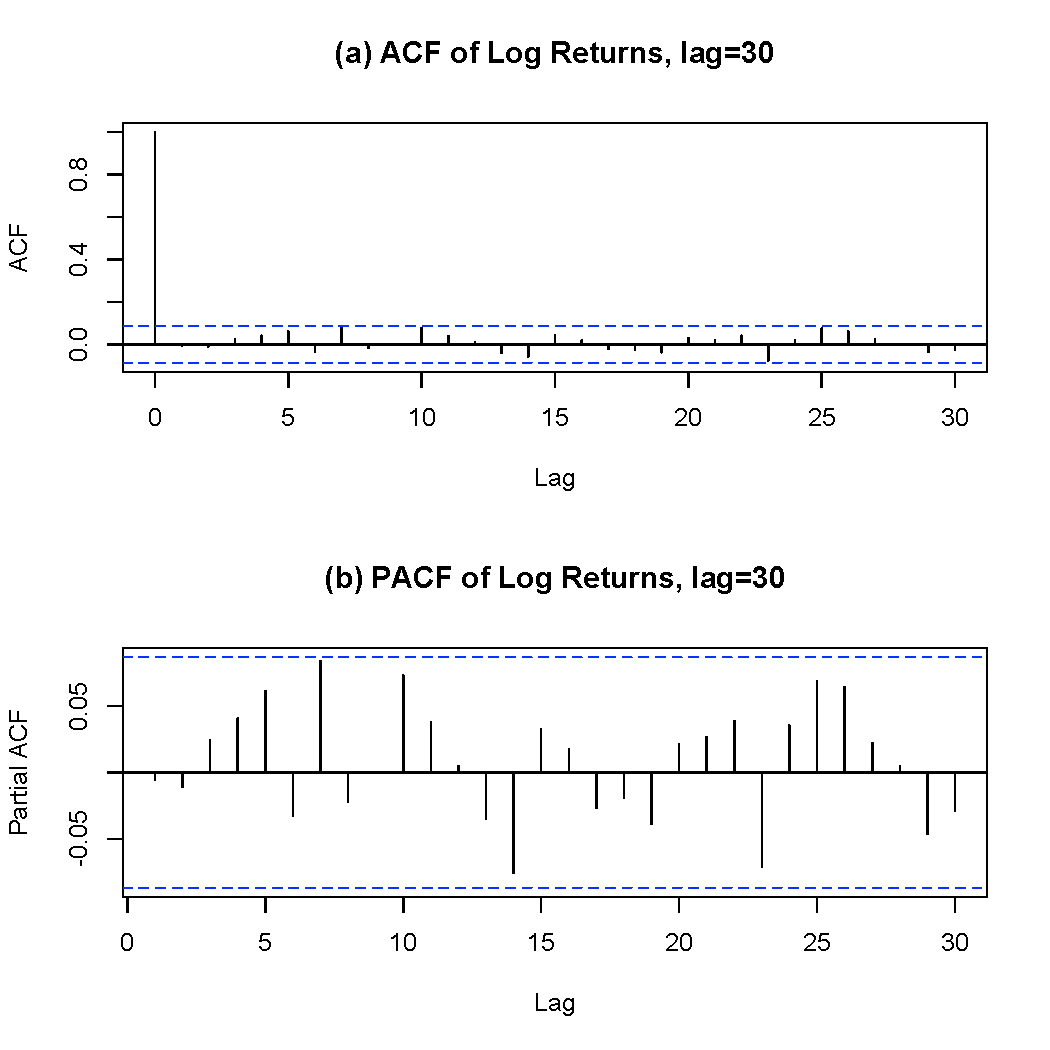
\includegraphics[scale=.6]{pacf}
  \caption[Comparing ACF with PACF]{(a) ACF function of AAPL log returns with 30-day lag. (b) PACF function of AAPL log returns with 30-day lag.}
  \label{figure:pacf}
\end{figure}

\subsubsection{Information Criterion Function}
Another way to determine the order $p$ of an AR process is by using a likelihood function such as the \emph{Akaike information criterion (AIC)}\index{Akaike information criterion (AIC)}, which measures goodness of fit of a model, and penalizes excessive use of parameters $k$.
\begin{equation}
AIC=\frac{-2}{n} \ln(\text{likelihood}) + \frac{2}{n} \times k,
\end{equation}
where the likelihood function is evaluated at the maximum likelihood estimates, \\
$n$ = sample size, \\
$k$ =  number of parameters.

\subsubsection{Goodness of Fit}
A conventional statistic to measure goodness of fit of a stationary model is $r^2$,
\begin{equation}
r^2 = 1 - \frac{\sum^T_{t=p+1}\hat{a}^2_t}{\sum^T_{t=p+1}(r_t-\bar{r})^2}
\end{equation}
where $\bar{r}= \left( \sum{T}{t=p+1} r_t\right) / (T-p)$. Yet, this only applies to a stationary time series. As a replacement, the \emph{adjusted $r^2$} is offered,
\begin{eqnarray*}
\text{Adj $r^2$} &=& 1 - \frac{\text{Variance of residuals}}{\text{Variance of $r_t$}} \\
&=& 1- \frac{\hat{\sigma}^2_a}{\hat{\sigma}^2_r}.
\end{eqnarray*}


\subsubsection{Forecasting}
Much of the purpose of \fts{} is forecasting. The AR($p$) model in \eqref{eq:arp} can be used to model a forecast. If we at time index $h$ and we forecast $r_{h+\ell}$, where $\ell \ge 1$, then $h$ is our \emph{forecast origin}\index{Forecast origin} and $\ell$ is our \emph{forecast horizon}\index{Forecast horizon}. Let $\hat{r}_h(\ell)$ be the forecast of $r_{h+\ell}$ using the minimum squared error loss function and $F_h$ is the collection of information at the forecast origin $h$. Then, the forecast $\hat{r}_k(\ell)$ is chosen such that
\[
E\{[r_{h+\ell} - \hat{r}_h(\ell)]^2 | F_h \} \le \min_g E[(r_{h+\ell}-g)^2 | F_h],
\]
where $g$ is a function of he information available at time $h$ (inclusive), that is, a function of $F_h$. We referred to $\hat{r}_h$ as the $\ell$-step ahead forecast of $r_t$, at the forecast origin $h$.

\margincomment[red]{The $\phi$ parameters are to be estimated from the data.}
\paragraph{1-Step Ahead Forecast.} Using \eqref{eq:arp}, we see
\[
r_{h+1} = \phi_0 + \phi_1 r_h + \cdots + \phi_p r_{h+1-p} + a_{h+1}.
\]
Under the minimum squared error loss function, the point forecast of $r_{h+1}$ given that $F_h=\{r_h, r_{h-1}, \ldots \}$ is the conditional expectation
\[
\hat{r}_h(1)=E(r_{h+1} | F_h) = \phi_0 + \sum^{p}_{i=1} \phi_i r_{h+1-i},
\]
and the associated forecast error is
\[
e_h(1)=r_{h+1} - \hat{r}_h(1) = a_{h+1}.
\]
The process can be extended to 2-step ahead and beyond by simple extension. The conditional expectation and forecast error are also adjusted accordingly.

\paragraph{Multistep Ahead Forecast.} A generalization of 1-step ahead forecast is an $\ell$-step ahead forecast
\begin{equation}
\hat{r}_h(\ell) = \phi_0 + \sum^{p}_{i=1} \phi_i \hat{r}_h(\ell-i),
\label{eq:multistep-forecast}
\end{equation}
where $\hat{r}_h(i)=r_{h+i}$ if $i \le 0$. This forecast can be computed recursively using forecasts $\hat{r}_h(i)$ for $i= \{1, \ldots, \ell-1 \}$. The $\ell$-step ahead forecast error is $e_h(\ell)=r_{h+\ell}-\hat{r}_h(\ell)$. It can be shown that for a stationary AR($p$) model, $\hat{r}_h(\ell)$ converges to $E(r_t)$ as $\ell \rightarrow \infty$, meaning that for such a series long-term point forecast approaches its unconditional mean. This property is \emph{mean reversion}\index{Mean reversion}, and appears in literature, notably in interest rate studies.

In an AR(1) model, the speed of mean reversion is measured by the \emph{half-life} defined as $k=\ln(0.5 / \left| \phi_1 \right| )$, which is defined as the number of periods required for the magnitude of the forecast to become one-half of the forecast origin. The variance of the forecast error approaches the unconditional variance of $r_t$.

We see in Figure~\ref{figure:gnp-acf} a plot of 176 observations of U.S. GNP changes. In panel (a), it appears that although the changes fluctuate, they tend to return to a central point indicated by the red dashed line, a point of mean reversion. The lag is changed from lag-1 to lag-2, and we observe a slight upward drift, which is consistent with our seeing that panel (a) has a mean slightly greater than zero (0.007741, actually). Next, we look for the presence of autocorrelation. The R code to examine GNP changes and ACF is very simple.

\ecaption{Examining GNP Changes and ACF function in R}
\begin{verbatim}
gnpdata=read.table("q-gnp4791.txt")
GNP=gnpdata[,1]
par(mfcol=c(2,2)) # put 4 plots on one page
plot(GNP,type="l",main="(a)") 
abline(mean(GNP),0, col="red",lty=4)
plot(GNP[1:175], GNP[2:176], main="(c)")
plot(GNP[1:174], GNP[3:176], main="(b)")
acf(GNP, lag=12, main="(d)") 

\end{verbatim}

\begin{figure}[tb]
  \centering
  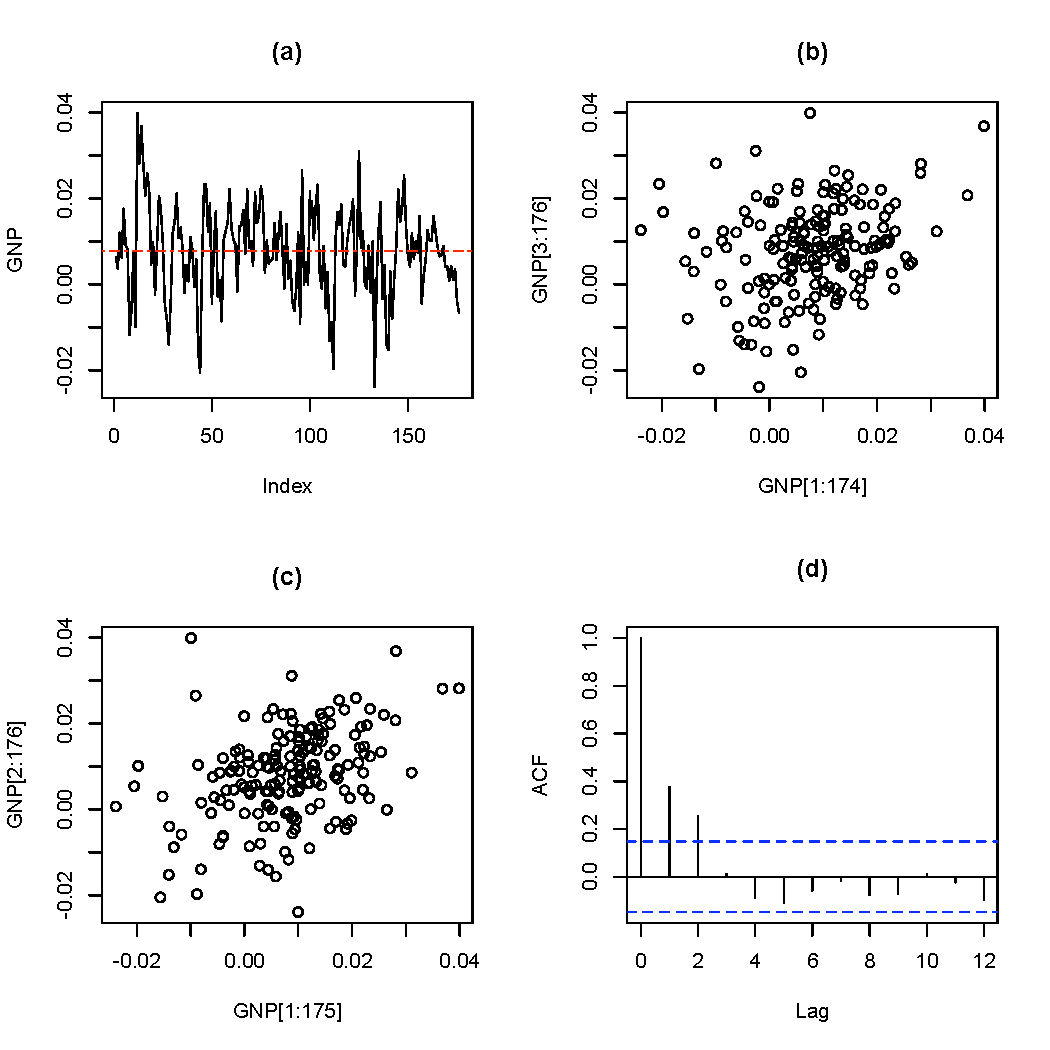
\includegraphics[scale=.65]{gnp-acf}
  \caption[Analysis of U.S. GNP with ACF function]{After plotting changes in U.S. GNP (a), we compare lag-1 (b), to lag-2 (c), and then see that the 12-period ACF function (d) finds autocorrelation at lag-1 and lag-2.}
  \label{figure:gnp-acf}
\end{figure}

\subsection{Simple Moving-Average Models}\index{Simple Moving-Average Models}
Another type of \fts{} model is the \emph{moving average} (MA) model. Initially, an MA model is understood as an AR model of infinite order
\[
r_t = \phi_0 + \phi_1 r_{t-1} + \cdots + \phi_{\infty} r_{\infty}.
\]
This is unrealistic because we have an infinite number of parameters. We will replace it with an MA($\ell$) model of finite order, specifically, $\ell$
\[
X_t = \varepsilon_t + \sum_{i=1}^\ell \theta_i \varepsilon_{t-i}.
\]

\paragraph{MA Models.} MA models are always weakly stationary because they are finite linear combinations of a white noise sequence for which the first two moments are time-invariant. To discover the order of an MA model, we may use an ACF function. We see from Figure~\ref{figure:pacf} what the 30-day lag looks like with AAPL log returns. Using that lag, we plot the log returns, its mean, and a 30-day moving average is superimposed in blue in Figure~\ref{figure:aapl-ret-ma30}.

\begin{figure}[tb]
  \centering
  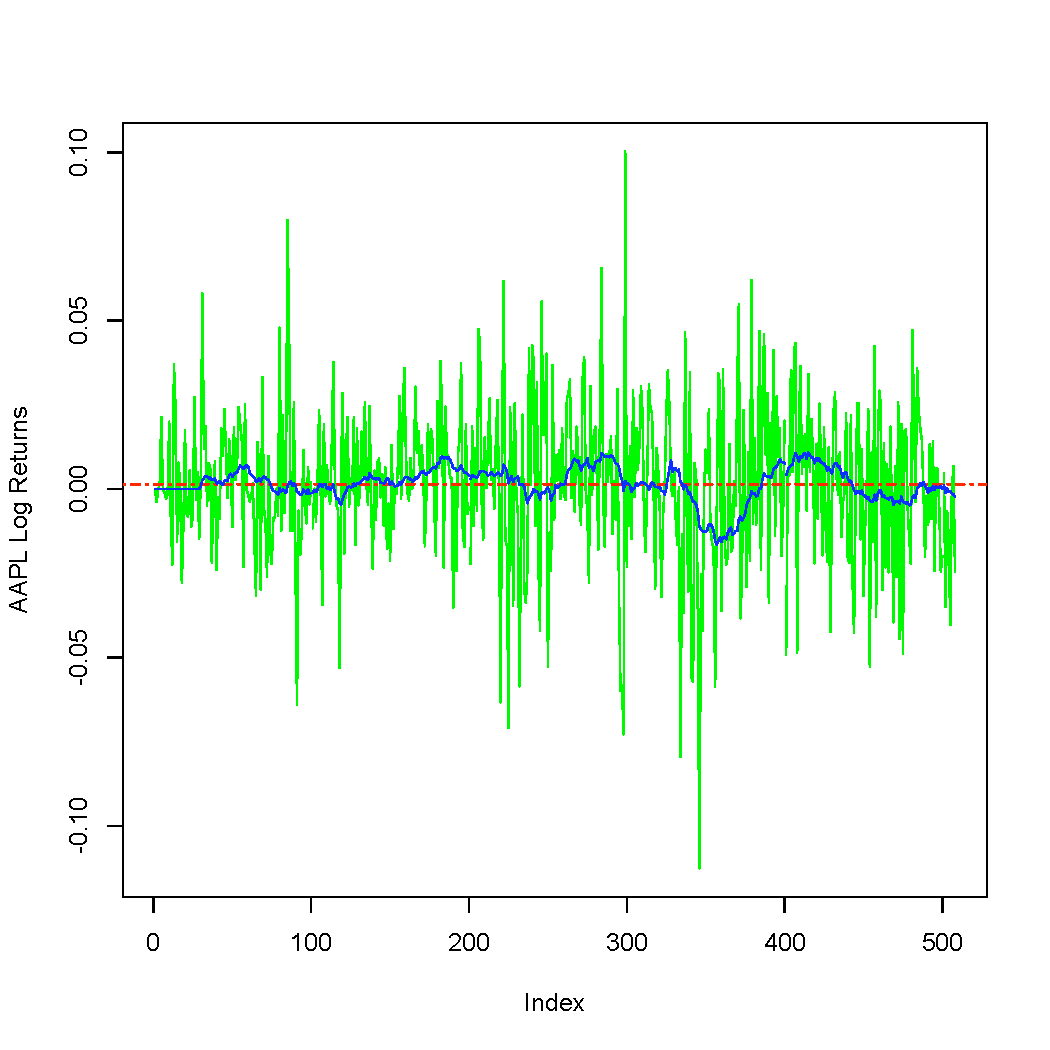
\includegraphics[scale=.6]{aapl-ret-ma30}
  \caption[AAPL Log Returns and MA(30)]{AAPL log return plotted in green. The mean plotted in red and dashed line. The 30-day moving average is superimposed in blue.}
  \label{figure:aapl-ret-ma30}
\end{figure}


\pagebreak
\subsection{Simple ARMA Models}\index{ARMA Models}
\margincomment{ARMA models are used with volatility modeling more than with returns series.}
Having briefly discussed both AR and MA models, we discover that a model of multiple order may be required to perform adequate modeling and forecasting. A remedy for this is the autoregressive moving-average (ARMA) model, which is a combined model that keeps the number of parameters small. It is also important to understand ARMA models as a building block to GARCH models, which are discussed in Section~\ref{garch}.

A time series $r_t$ follows an ARMA(1,1) model if it satisfies
\begin{equation}
r_t - \phi_1 r_{t-1} = \phi_0 + a_t - \theta_0 + a_t - \theta_1 a_{t-1},
\label{eq:arma1-1}
\end{equation}
where $\{a_t\}$ is a white noise series. The left-hand side of \eqref{eq:arma1-1} is the AR component and the right-hand side is the MA component. The constant term is $\phi_0$. To avoid cancellation of both sides, which would make \eqref{eq:arma1-1} a white noise series, we require that $\phi_1 \ne \theta_1$.

\paragraph{ARMA(1,1) Models.} Since ARMA(1,1) models are generalizations of AR(1) models with modifications to allow inclusion of a MA(1) component, we already know much about these models, such as the stationarity condition is the same. There is a notable differences, the ACF of an ARMA(1,1) model looks like a AR(1) model except that the exponential decay starts with lag 2 instead of lag 1. The general form of an ARMA($p,q$) model is
\[
r_t = \phi_0 + \sum^p_{i=1} \phi_i r_{t-1} + a_t - \sum^q_{i=1} \theta_i a_{t-i},
\]
where $\{a_t\}$ is a white noise series and $p$ and $q$ are non-negative integers.

Using ACF and PACF are not very useful in determining the order of an ARMA model. \citeA{tsaytiao1984eacf} propose an alternative approach, which is known as the \emph{extended autocorrelation function} (EACF).\index{Extended Autocorrelation Function \\(EACF)} This function is used to specify the order of an ARMA process. The aim is to derive the MA component from a consistent estimate of the AR component of an ARMA model.

\paragraph{Forecasting with ARMA.} A 1-step ahead forecast $r_{h+1}$ of an ARMA model is
\[
\hat{r}_h(1)=E(r_{h+1}|F_h)=\phi_0 + \sum^p_{i=1} \phi_i r_{h+1-i} - \sum^q_{i=1} \theta_i a_{h+1-i},
\]
where $h$ is the forecast origin, and $F_h$ is the available information.

\subsection{Unit-Root Nonstationarity}\index{Unit-Root Nonstationarity}
Several types of \fts{} are nonstationary, such as interest rates, foreign exchange currency rates, and asset price series because they have no fixed level of price. This condition is all referred to as \emph{unit-root nonsationarity}.  The best known example of this is a random-walk model.

A random walk is a time series $\{p_t\}$ that satisfies the condition
\begin{equation}
p_t = p_{t-1}+a_t,
\label{eq:random-walk}
\end{equation}
where $p_0$ is the starting value and $\{a_t\}$ is white noise.

Using a simple R statement, \texttt{plot(cumsum(rnorm(20000)),type="l")} used three times, we create three random walks that seem to converge in Figure~\ref{figure:three-walks}. One obvious problem is that the price time series drops below zero on several occasions. A nominal price or rate will never be below zero, but a \emph{real rate}, one compared to another over time, may become negative.
\begin{figure}[tb]
  \centering
  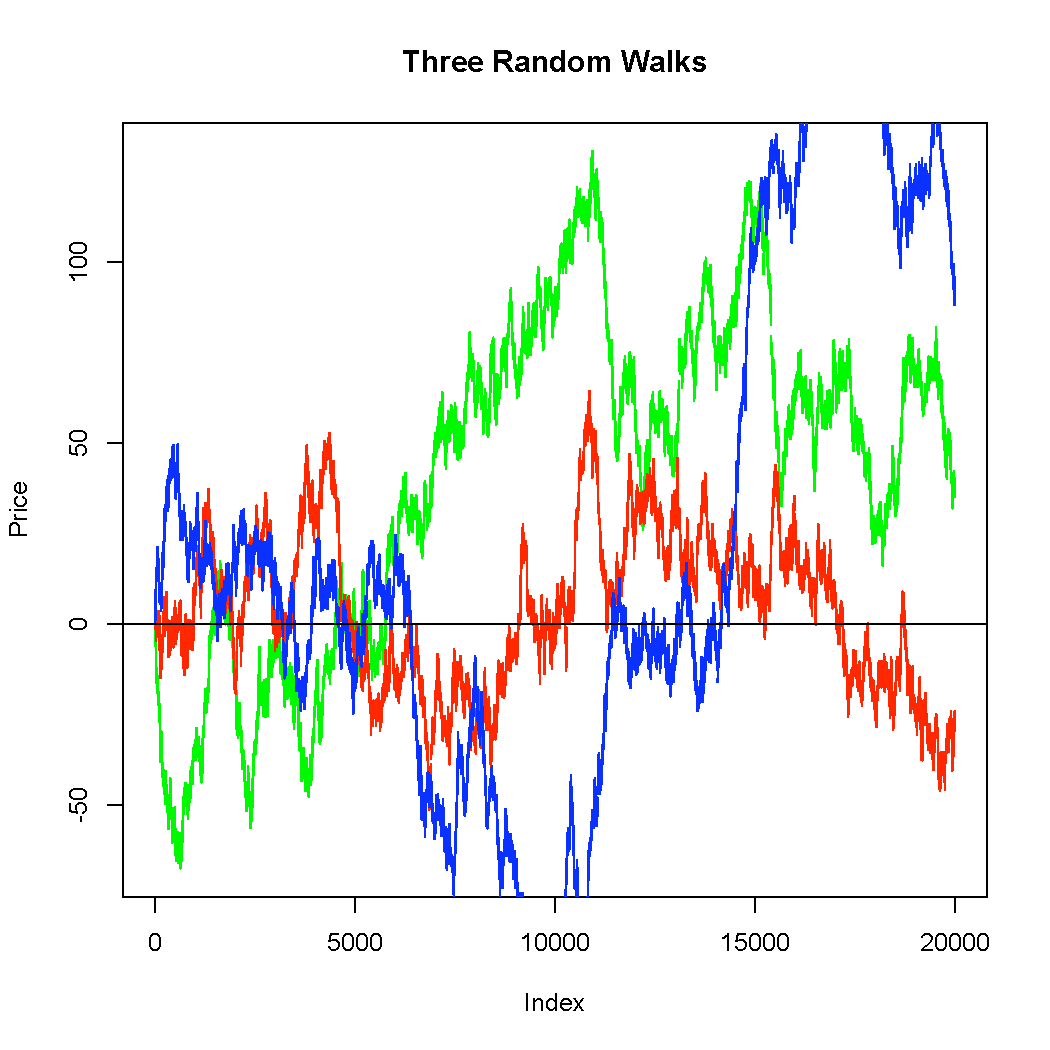
\includegraphics[scale=.6]{three-walks}
  \caption[Three Random Walks, no Drift]{Three random walks, with no drift, yet they seem to converge.}
  \label{figure:three-walks}
\end{figure}

If we treat \eqref{eq:random-walk} as a kind of AR(1) model, then the coefficient of $p_{t-1}$ is one (\emph{or unity}), which does not satisfy the weak stationarity condition of an AR(1) model. Therefore, a random-walk series is a unit-root nonstationary time series.  This kind of series is not predictable or mean-reverting.

The MA representation of \eqref{eq:random-walk} is
\[
p_t = a_t + a_{t-1} + a_{t-2} + \cdots,
\]
which may continue indefinitely. The $\ell$-step ahead forecast error is
\[
e_h(\ell) = a_{h+\ell} + \cdots + a_{h+1},
\]
which means that $\text{Var}[e_h(\ell)] = \ell \sigma^2$, and it diverges to infinity as $\ell \to \infty$. Again, this model is not predictable because the usefulness of the point forecast $\hat{p}_h(\ell)$ diminishes as $\ell$ increases.

\paragraph{Random Walk with Drift.} Observing markets, it becomes clear that the log return series exhibits a positive mean, which would indicate some form of drift.
\begin{equation}
p_t = \mu +p_{t-1} + a_t,
\end{equation}
where $\mu=E(p_t - p_{t-1})$ and $\{a_t\}$ is white noise. The $\mu$ term is vital to the model because it represents the time trend of the log price $p_t$, and is referred to as the \emph{drift}.

\subsubsection{Trend-Stationary Time Series}
A model that is related to random walk with drift is the trend-stationary time series model
\[
p_t = \beta_0 + \beta_1 t+r_t
\]
where $r_t$ is a stationary time series, such as a stationary AR($p$) series. We observe that $p_t$ grows in time on a linear scale $\beta_1$.

\subsubsection{Unit-Root Nonstationary Models}
Modifying an ARMA model by allowing the AR polynomial to have 1 as a characteristic root, the model becomes the autoregressive integrated moving-average (ARIMA)\index{Autoregressive Integrated\\ Moving-Average (ARIMA)} model. A common way to handle unit-root nonstationarity is by \emph{differencing}\index{Differencing}.

\paragraph{Differencing.} Price time series are seen as nonstationary, but log returns are stationary. A way to transform a non-stationary model into a stationary one is by \emph{differencing}. The first difference series of $y_t$ is
\[
c_t = y_t - y_{t-1}.
\]
Also, if $s_t$ follows an ARMA($p,q$) model, then $y_t$ is an ARIMA($p,2,q$) process.

\paragraph{Unit-Root Test.}\index{Unit-root test} To test whether a log price series $p_t$ follows random walk or random walk with drift, we use
\begin{subequations}
	\begin{eqnarray}
	p_t &=& \phi_1 p_{t-1} + e_t, \label{eq:unit-root-a} \\
	 &=& \phi_0 + \phi_1 p_{t-1} + e_t \label{eq:unit-root-b}
	\end{eqnarray}
\end{subequations}
where $e_t$ is an error term comprising white noise, and we may using either \eqref{eq:unit-root-a} or \eqref{eq:unit-root-b} to examine the unit testing problem, which is set up as the \emph{Dickey-Fuller Test.}\index{Dickey-Fuller Test}\\
\begin{eqnarray*}
H_0: \phi_1 = 1 \\
H_a: \phi_1 < 1
\end{eqnarray*}
The test statistic is a $t$-ratio of least square estimate of $\phi_1$. For instance, the least square method for \eqref{eq:unit-root-a} is
\[
\hat{\phi}_1 = \frac{\sum^T_{t=1}p_{t-1}p_t}{\sum^T_{t=1}p^2_{t-1}}, \qquad
\hat{\sigma}^2_e = \frac{\sum^T_{t=1}(p_t-\hat{\phi}_1 p_{t-1})^2}{T-1},
\]
where $p_0=0$ and $T$ is the sample size. The Dickey-Fuller test $t$-ratio is
\[
DF \equiv \text{$t$-ratio} = \frac{\hat{\phi}_1-1}{\text{std}(\hat{\phi}_1)} 
= \frac{\sum^T_{t=1}p_{t-1}e_t}{\hat{\sigma}_e \sqrt{\sum^T_{t=1}p^2_{t-1}}}
\]

When modeling economic time series, it is better to use ARIMA($p,d,q$) than the simpler \eqref{eq:unit-root-b}, although AR($p$) models are also often used.

\paragraph{Testing ARIMA Models.} The three components $(p, d, q)$ of ARIMA are the AR order $p$, the degree of differencing $d$, and the MA order $q$. Using the R functions \texttt{arima} and \texttt{AIC} we will test several combinations of an ARIMA($p,d,q$) model and get an AIC value for each. The smaller the AIC, the better the model fits the data.

\ecaption{Testing ARIMA Models in R}
\begin{verbatim}
# Test AR order p by itself: ARIMA(p,0,0)
model100<-arima(aapl$Close,order=c(1,0,0))
model200<-arima(aapl$Close,order=c(2,0,0))
AIC(model100, model200)

# Test the MA order q by itself: ARIMA(0,0,q)
model001<-arima(aapl$Close,order=c(0,0,1))
model002<-arima(aapl$Close,order=c(0,0,2))
AIC(model001,model002)

# Now hold AR constant, change MA
model100<-arima(aapl$Close,order=c(1,0,0))
model101<-arima(aapl$Close,order=c(1,0,1))
model102<-arima(aapl$Close,order=c(1,0,2))
AIC(model100,model101,model102)

# Test the degree of differencing d
model100<-arima(aapl$Close,order=c(1,0,0))
model110<-arima(aapl$Close,order=c(1,1,0))
AIC(model100,model110)
\end{verbatim}

\subsection{Seasonal Models}\index{Seasonal Models}
\begin{figure}[tb]
  \centering
  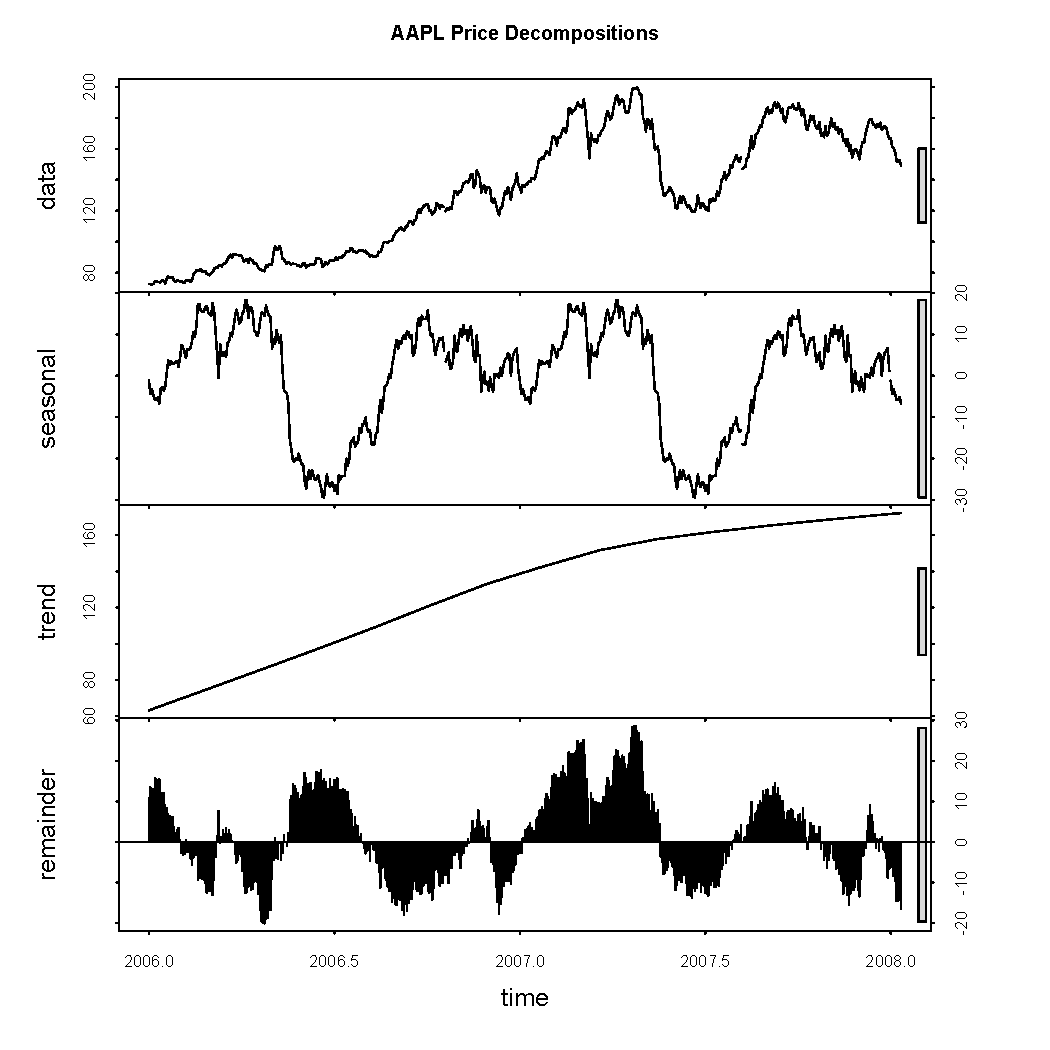
\includegraphics[scale=.7]{aapl-stl}
  \caption{AAPL Price Series Decomposition}
  \label{figure:aapl-stl}
\end{figure}

We can use R to create a decomposition of the AAPL time series, which displays the data, seasonal pattern, trend, and the remainder. The decomposition is displayed in Figure~\ref{figure:aapl-stl}. There are four factors that influence time series as seen in Table~\ref{tab:factors-ts}. The R code follows.
\ecaption{Time Series Decomposition in R}
\begin{verbatim}
aaplts<-ts(aapl$Close,start=c(2006,1),frequency=250)
decomp<-stl(aaplts,"periodic")
plot(decomp)
\end{verbatim}

\begin{table}[htbp]
	\centering
	\begin{tabular}{llll}
	\toprule
	Factor & Definition & Duration \\
	\hline
	Trend & Overall persistent long-term movement & Years \\
	Seasonal & Regular pattern of periodic fluctuations per year & Within 12 mo. \\
	& & (weekly, annually, \textit{etc.}) \\
	Cyclical &	Repeating up/down swings & Several (2--10) years \\
	Irregular &	 Erratic, random variation & Non-repeating \\
	\bottomrule
	\end{tabular}
	\caption{Factors Influencing Time Series}
	\label{tab:factors-ts}
\end{table}

\subsubsection{Seasonal Differencing with Dummy Variables}\label{perform-ts}
We will take data from the 2004 \emph{Economic Report of the President} which contain many variables, but we are only concerned with, \textit{i3} the 3-month T-bill rate, \textit{inf} the annual inflation rate, and \textit{def} the federal budget deficit as a percentage of GDP. We want to calculate $\beta$ values for the equation,
\begin{equation}
\widehat{i3_t} = \beta_0 + \beta_1 inf_t + \beta_2 def_t.
\label{eq:ts-regress}
\end{equation}

We load the MATLAB data file \texttt{econrep} which has a matrix named \texttt{intdef}. The remaining steps to get our $\beta$ values are required to perform matrix division.

\ecaption{Time Series Regression in MATLAB}
\begin{verbatim}
     load econrep
     i3=intdef(:,2);
     inf=intdef(:,3);
     def=intdef(:,6);
     A=[ones(size(inf)) inf def];
     x=A\i3
     
     x =
         1.7333
         0.6059
         0.5131
\end{verbatim}

which allows us to fill in constants for \eqref{eq:ts-regress},
\[
\widehat{i3_t} = 1.7333 + 0.6059 \times inf_t + 0.5131 \times def_t.
\]
Next, we want to determine the $r^2$ value of this regression equation. However, we want to obtain an \emph{adjusted} $r^2$,
\begin{equation}
r^2_{adj} = 1- \Big( (1-r^2)\frac{n-1}{n-k-1} \Big),
\label{eq:adj-rsquared}
\end{equation}
where $n$ is sample size, and $k$ is degrees of freedom in the regression. This allows us to compare regressions with different numbers of independent variables. Adjusting $r^2$ in \eqref{eq:adj-rsquared} allows us to account for the number of parameters used in the regression.

\begin{verbatim}
     yhat=x(1) + x(2).*inf + x(3).*def;
     sst=sum((i3-mean(i3)).^2);
     sse=sum((yhat-mean(i3)).^2);
     ssr=sum((yhat-i3).^2);
     r_squared=sse/sst;
     n=size(i3,1);
     k=size(x,1)-1;
     adj_r2=1-((1-r_squared).*(n-1)/(n-k-1))
\end{verbatim}

We see that our $r^2=0.6021$ and adjusted $r^2=0.5871$.

\paragraph{Dummy Variables.}\index{Binary Variable|see{Dummy Variable}}\index{Dummy Variable}\label{dummy-variable}
Binary variables are also known as \emph{dummy variables}. In order to include an observed qualitative factor, we need to pick a variable that indicates what is represented by the number 1. Choosing $female=1$ is more clear than $gender=1$, which tells us nothing about what the value of 1 represents. %We can add a qualitative factor to \eqref{eq:ts-regress} by adding a dummy variable, giving us
\paragraph{Ordinal Variables.}Some qualitative variables are \emph{ordinal}, that is, they measure a factor that has more than two values. If we want to use season of the year as an independent variable, we need four values (Winter, Spring, Summer, Fall). It makes little sense to assign $S=1$ to Winter, and $S=2$ to Spring because Spring does not represent any quantity that is double the value of Winter.  Instead, we may assign a variable for each season (Table~\ref{tab:ord-variable}), so that we have,
\[
\hat{y} = \beta_0 + \delta_1 S_1 + \delta_2 S_2 + \delta_3 S_3 +\delta_4 S_4 + \epsilon.
\]

\begin{table}[tbp]
	\centering
	\begin{tabular}{lc}
	\toprule
	Season & Variables \\
	\hline
	Winter & $\mathbf{S_1=1}; S_2 = 0; S_3 = 0; S_4 = 0$ \\
	Spring & $S_1=0; \mathbf{S_2 = 1}; S_3 = 0; S_4 = 0$ \\
	Summer & $S_1=0; S_2 = 0; \mathbf{S_3 = 1}; S_4 = 0$ \\
	Fall & $S_1=0; S_2 = 0; S_3 = 0; \mathbf{S_4 = 1}$ \\
	\bottomrule
	\end{tabular}
   \caption{Ordinal Variable Setting}
   \label{tab:ord-variable}
\end{table}

One value they can add to time series analysis is in the form of an \emph{event study}.\index{Event Study} The variable can indicate the period in which a specific event occurred. If we add a dummy variable to \eqref{eq:ts-regress} that indicates if Congress has enacted a certain law,
\[
\widehat{i3_t} = \beta_0 + \beta_1 inf_t + \beta_2 def_t + \beta_3 d_t,
\]
then, with that dummy variable $d_t$ we can observe the effect of the law by measuring the estimators with the variable and without it.

\paragraph{Index Numbers.}
To construct an event study, we must often work with an \emph{index number}\index{Index Number}.  The Consumer Price Index (CPI), ``is a measure of changes in prices for purchases made by urban consumers only'' \cite[p. 91]{rogers-1998}. Essentially, it is the price of a specific basket of consumer goods at a specific point in time. The Bureau of Labor Statistics\index{Bureau of Labor Statistics (BLS)} publishes a national number as well as several regions CPI numbers.

An index number such as the CPI-U\footnote{The U.S. Department of Labor publishes a monthly ``All Urban Consumers'' Consumer Price Index (CPI-U) based on U.S. city average of a basket of consumer goods. The CPI website is located at \\ \texttt{http://www.bls.gov/cpi/home.htm}} means nothing on its own; the August 2008 level is 219.086, and is -0.4 percent lower than in the previous month. However, its value comes from comparing it to a \emph{base period}\index{Base Period}  which has a \emph{base value}\index{Base Value}.  Our August 2008 CPI-U has a base period of 1982--1984, and a base value of 100. From this point, we can determine the change in price level for consumers over a span of time. Additionally, we can adjust \emph{nominal dollars} into \emph{real dollars} by factoring inflation as measured by CPI changes.

Having made any adjustments using index numbers to our time series data, we may use them in time series regressions without distorting their value.

\subsubsection{Trend and Seasonality}\index{Time Series!trend and seasonality}
Referring back to Figure~\ref{figure:aapl-stl}, we see that econometric models calculate the level, trend and seasonality and combine them to arrive at a forecast. It is not possible to understand the nature of trend and seasonality simply by viewing the data in the graphical screen. Decomposing time series data into trend and seasonality provides insights into the patterns of these components. This helps us choose the right forecast strategy or in setting the
parameters for a particular strategy.

Isolating the trend component requires neutralizing the seasonal effect in the data. If the data has a 12 period seasonality, computing a 12 period \emph{moving average} neutralizes the effect of seasonality. With a history of 24--36 months, we can calculate the trend for 13--25 months. Viewing the trend graphically provides insights into the way trend is changing over the analysis period. We can assess from this graph if the short term trend is in line with the long term trend. The short term trend is relevant for operational decisions like trading whereas the long term trend would be relevant for annual budgeting and other capital expenditure decisions.

Since the time series is a combination of trend, seasonality and randomness, subtracting the trend from the time series will leave us with seasonality and randomness. The seasonal patterns can be viewed graphically at different aggregate levels. If the time series has
seasonality, one will be viewing recurring patterns at periodic intervals. If there is no seasonality, there will not be any recurring patterns but only random patterns.

%\paragraph{Durbin-Watson Statistic.}\index{Durbin-Watson statistic}
%\subsection{Fractionally Differenced Models}\index{Fractionally Differenced Models}
%\subsection{Long-Memory Modeling}
\section{Conditional Heteroskedastic Models}\label{Conditional Heteroskedastic}
\paragraph{Primary Text Reading.} \citeA[chap. 3]{tsay2005aft}\index{Tsay, Ruey}

Up to this point, we have focused on modeling assets returns or forecasting their prices. When analyzing \fts{}, we may also want to analyze the \emph{volatility} or, the conditional standard deviation, of the asset. Since volatility is not directly experienced, we must find a substitute for it. We can look at an option pricing model that uses volatility as an input.

The \emph{implied volatility}\index{Implied volatility} of an option contract is the volatility implied by the market price of the option based on an option pricing model. It is the volatility that, given a particular pricing model, yields a theoretical value for the option equal to the current market price. Implied volatility, a forward-looking measure, differs from historical volatility because the latter is calculated from known past prices of a security.

One model, which requires conditional volatility as one of its inputs, is the Black-Scholes option pricing model,\index{Black-Scholes option pricing model}
\begin{subequations}
	\begin{eqnarray}
	C(S,T) &=& S\Phi(d_1) - Ke^{-rT}\Phi(d_2) \label{eq:bs-call} \\
	P(S,T) &=& Ke^{-rT}\Phi(-d_2) - S\Phi(-d_1) \label{eq:bs-put}
	\end{eqnarray}
\end{subequations}
where,
\begin{eqnarray*}
d_1 &=& \frac{\ln(S/K) + (r + \sigma^2/2)T}{\sigma\sqrt{T}} \notag \\
d_2 &=& d_1 - \sigma\sqrt{T} \notag \\
\Phi(\cdot) &=& \text{c.d.f. of the Normal Distribution, \eqref{eq:cdf}}. \notag
\end{eqnarray*}
Using this closed-form solution, we can obtain the price for either a call option \eqref{eq:bs-call} or a put option \eqref{eq:bs-put}\footnote{A \emph{call option} is a contract that gives the holder the right to \textbf{buy} a certain quantity of an underlying security from the writer of the option, at a specified price (the strike price) up to a specified date (the expiration date). 
A \emph{put option} is a contract that gives the holder the right to \textbf{sell} a certain quantity of an underlying security to the writer of the option, at a specified price up to a specified date.
}.
Similarly, if we have the option price, and all other inputs except the volatility, we can calculate the implied volatility by entering a value that would satisfy the equation. However, to do so may be relying upon the model (and its unrealistic assumptions) too much.

\paragraph{Volatility.} It is a difficult task to measure volatility of an asset return. Although the volatility may exist in a continuous form, with no sudden jumps, it may remain low for a period and then shift upward. Depending upon the asset, and whether it rose or fell in price, a major price change in the underlying security may affect volatility differently. To be certain, volatility changes, and it can be rapid and difficult to observe directly.

\margincomment[red]{Different volatility models make different assumptions about $\sigma^2_t$.}
To measure volatility, we need to model the changes in variance $\sigma^2_t$ in the asset return time series. The various conditional heteroskedastic models differ in how this variance changes in time. The evolution of $\sigma^2_t$ is deterministic in some models, such as the GARCH model, yet \emph{stochastic volatility}\index{Stochastic Volatility model} models exist also.

\subsection{Building a Volatility Model}
The basic structure of volatility modeling is
\[
r_t = \mu_t + a_t, \quad \mu_t = \phi_0 + \sum^k_{i=1}\beta_i x_{it} + \sum^p_{i=1}\phi_i r_{t-i}
- \sum^q_{i=1}\theta_i a_{t-i},
\]
and volatility models are concerned with time-evolution of
\[
\sigma^2_t = \text{Var} \left(r_t | F_{t-1} \right) = \text{Var} \left(a_t | F_{t-1} \right).
\]
Volatility model building requires four steps,
\begin{enumerate}
\item Create a mean equation and test for serial dependence in the \fts{}, and calibrate an AR or ARMA model to remove autocorrelation. For many asset returns, this is as simple as removing the sample mean from the data, and adding qualitative variables, as described in Section~\ref{dummy-variable}.
\item Test for ARCH effects with the residuals from the previous step.
\item If ARCH effects are statistically significant, choose a volatility model, and perform a joint estimation of the mean and volatility equations.
\item Refine the model if needed.
\end{enumerate}

\subsubsection{ARCH Effects}
If we denote $a_t = r_t - \mu_t$ as the residuals of the mean equation, then the squared series $a^2_t$ is used to check for conditional heteroskedacity. These are the \emph{ARCH effects}. There are two different tests available. We can apply the Ljung-Box statistic\index{Ljung-Box test} $Q(m)$ to  $\{a^2_t\}$ using as the null hypothesis that the first $m$ lags are zero. Another test is the \emph{Lagrange multiplier test}\index{Lagrange multiplier test}, which is equivalent to $F$ statistic for testing $\alpha_i=0 \quad (i=1,\ldots,m)$ in a linear regression
\[
a^2_t = \alpha_0 +\alpha_1 \alpha^2_{t-1}+\cdots+\alpha_m\alpha^2_{t-m}+e_t, \quad 
t=m+1,\ldots,T,
\]
where $e_t$ is the error term, $m$ is a specific positive integer, and $T$ is the sample size. The null hypothesis is $H_0: \alpha_1= \cdots a_m = 0$. Next, we need to define $SSR_0$ and $SSR_1$
\begin{eqnarray*}
SSR_0 &=& \sum^T_{t=m+1} (a^2_t - \bar{\omega})^2, \\
SSR_1 &=& \sum^T_{t=m+1} \hat{e}^2_t, 
\end{eqnarray*}
where $\bar{\omega}=(1/T)\sum^T_{t=1}a^2_t$ is the sample mean of $a^2_t$ and  $\hat{e}^t$ is the least squares residual of the prior linear regression. The $F$-test is then
\[
F=\frac{(SSR_0-SSR_1)/m}{SSR_1/(T-2m-1)}.
\]

\subsubsection{ARCH Model}
An \emph{autoregressive conditional heteroskedasticity} (ARCH) model\index{Autoregressive Conditional \\ Heteroskedasticity (ARCH) model} considers the variance of the current error term to be a function of the variances of the previous time period's error terms \cite{engle1982arch}.  ARCH relates the error variance to the square of a previous period's error. It is employed commonly in modeling financial time series that exhibit time-varying volatility clustering, which are periods of swings followed by periods of relative calm. The shock $a_t$ of an asset return is serially uncorrelated, but dependent; and the dependence can be described by a simple quadratic function of its lagged values.

%TODO: Maybe show asset returns and squared series for ARCH effect.

Specifically, let $\epsilon_t$  denote the returns (or return residuals, net of a mean process) and assume that $\epsilon_t=\sigma_t z_t$, where $z_t\sim iid~ N(0,1)$  and where the series $\sigma_t^2$  are modeled by
\[
\sigma_t^2=\alpha_0+\alpha_1 \epsilon_{t-1}^2+\cdots+\alpha_q \epsilon_{t-q}^2 = \alpha_0 + \sum_{i=1}^q \alpha_{i} \epsilon_{t-i}^2 
\]
and where $\alpha_0>0$  and $\alpha_i\ge 0,~i>0$.

\subsubsection{ARCH($q$) Model Specification}

An ARCH($q$) model can be estimated using ordinary least squares. A methodology to test for the lag length of ARCH errors using the Lagrange multiplier test was proposed by \citeA{engle1982arch}. Estimate the best fitting AR($q$) model
\[
y_t = a_0 + a_1 y_{t-1} + \cdots + a_q y_{t-q} + \epsilon_t = a_0 + \sum_{i=1}^q a_i y_{t-i} + \epsilon_t 
\]
Obtain the squares of the error $\hat{\epsilon}^2$  and regress them on a constant and $q$ lagged values,
\[
\hat \epsilon_t^2 = \hat \alpha_0 + \sum_{i=1}^{q} \hat \alpha_i \hat \epsilon_{t-i}^2
\]
where $q$ is the length of ARCH lags.

The null hypothesis is that, in the absence of ARCH effects, we have $\alpha_i = 0$ for all $i = \{1, \ldots, q\}$. The alternative hypothesis is that, in the presence of ARCH effects, at least one of the estimated $\alpha_i$ coefficients must be significant. In a sample of $T$ residuals under the null hypothesis of no ARCH errors, the test statistic $TR^2$ follows $\chi^2$ distribution with $q$ degrees of freedom. If $TR^2$ is greater than the chi-square table value, we reject the null hypothesis and conclude there is an ARCH effect in the ARMA model. If $TR^2$ is smaller than the chi-square table value, we accept the null hypothesis.

\paragraph{Model Building.}
%TODO: Test this code and expand on it.
Using the R library \texttt{FinTS}\index{FinTS@\texttt{FinTS} (library in R)}\footnote{Rmetrics has many other excellent functions in the \texttt{fSeries} package \cite{fseries-R}. A description of the many packages available from Rmetrics is at \texttt{http://www.rmetrics.org/rmetricsPackages.htm} and are available on CRAN.}
\cite{fints-R}, we can perform the Lagrange Multiplier (LM) test for autoregressive conditional heteroscedasticity (ARCH).
\ecaption{ARCH Test using R library, \texttt{FinTS}}
\begin{verbatim}
data(m.intc7303)
intcLM <- ArchTest(log(1+as.numeric(m.intc7303)), lag=12)
# Matches answer on Tsay (p. 102)
\end{verbatim}

\paragraph{Drawbacks of ARCH.} The ARCH model assume that positive and negative shocks have the same effect on volatility because it depends on the square of the previous shocks. This is not realistic. The ARCH model is not very helpful in finding the source of variation within a \fts{}. Also, the model responds slower to large isolated shocks.

\subsection{GARCH}\index{Generalized Autoregressive Conditional\\Heteroskedasticity (GARCH) model}\label{garch}
By comparison, ARCH models are simple, although the number of required parameters makes it difficult to calibrate. Next, we examine generalizations of ARCH to model volatility.
If an ARMA model is assumed for the error variance, the model is a generalized autoregressive conditional heteroskedasticity model \cite{bollerslev1986garch}. In such a case, the GARCH($m, s$) model, where $m$ is the order of the GARCH terms $\sigma^2$ and $s$ is the order of the ARCH terms $\epsilon^2$, is given by
\begin{eqnarray*}
\sigma_t^2&=&\alpha_0 + \alpha_1 \epsilon_{t-1}^2 + \cdots + \alpha_s \epsilon_{t-s}^2 + \beta_1 \sigma_{t-1}^2 + \cdots + \beta_m\sigma_{t-p}^2 \\
&=& \alpha_0 + \sum_{i=1}^q \alpha_i \epsilon_{t-i}^2 + \sum_{i=1}^m \beta_i \sigma_{t-i}^2.
\end{eqnarray*}
So that, the GARCH($m,s$) model is
\begin{equation}
a^2_t = \alpha_0 + \sum^{\max(m,s)}_{i=1} (\alpha_i + \beta_i) a^2_{t-i}+\eta_t
- \sum^s_{j=1} \beta_j \eta_{t-j}.
\label{eq:garch}
\end{equation}

\subsubsection{GARCH($m, s$) Model Specification}
The lag length $p$ of a GARCH process is established in three steps,
\begin{enumerate}
\item Estimate the best fitting AR($q$) model
\[
y_t = a_0 + a_1 y_{t-1} + \cdots + a_q y_{t-q} + \epsilon_t = a_0 + \sum_{i=1}^q a_i y_{t-i} + \epsilon_t 
\]
\item Compute and plot the autocorrelations of $\epsilon^2$ by 
\[
\rho = {{\sum^T_{t=i+1} (\hat \epsilon^2_t - \hat \sigma^2_t) (\hat \epsilon^2_{t-1} - \hat \sigma^2_{t-1})} \over {\sum^2_{t=1} (\hat \epsilon^2_t - \hat \sigma^2_t)^2}} 
\]
\item The asymptotic, large sample, standard deviation of $\rho(i)$ is $T^{-\frac{1}{2}}$. Individual values that are larger than this indicate GARCH errors. To estimate the total number of lags, use the Ljung-Box test until the value of the these are less than a 5\% significant. The Ljung-Box $Q$-statistic follows $\chi^2$ distribution with $n$ degrees of freedom if the squared residuals $\epsilon^2_t$  are uncorrelated. It is recommended to consider up to $T/4$ values of $n$. The null hypothesis states that there are ARCH or GARCH errors. Therefore, rejecting the null means that there are no such errors in the conditional variance.
\end{enumerate}

Specifying the order of a GARCH model is not easy, which is why lower order models such as GARCH(1,1), GARCH(1,2), or GARCH(2,1) are usually used. As long as the starting volatility is known, the conditional maximum likelihood method will work.

\paragraph{Forecasting with GARCH.}
Since volatility is not directly observable, testing and calibrating GARCH methods can be difficult. Often, one of the best ways to test a GARCH model for forecasting is to compare in-sample and out-of-sample results of volatility forecasts $\sigma^2_h(\ell)$ compared to shock $a^2_{h+\ell}$.

Forecasting with \eqref{eq:garch} can employ a similar method used when forecasting \eqref{eq:arma1-1}. Pursue the first parameter and seek the lowest AIC value, then hold that parameter constant while changing the second parameter. Sometimes, it may be helpful to go back and change the first parameter again after obtaining the second.

We can use a few R functions from the \texttt{fArma} library \cite{farma-R}, \texttt{fGarch} library \cite{fgarch-R}, and the \texttt{fSeries} library \cite{fseries-R} to examine GARCH models. The fit is displayed in Figure~\ref{figure:conditional-sd}.
\ecaption{GARCH Model Fitting in R}
\begin{verbatim}
spxm<-read.csv("SPX-M.csv", header=T)
spxts<-ts(spxm$Adj.Close, start=c(1950,1), frequency=12)
plot(spxts)

spxG<-garchFit(~garch(1, 1), data = spxts)
plot(spxG) # There are 13 different charts to choose from.
spxG@title
\end{verbatim}

With these functions, we can model the monthly volatility of the S\&P 500 Index with \texttt{fGarch}\index{fGarch@\texttt{fGarch} (library in R)} by starting with a GARCH(1,1) model. The \texttt{garchFit} function generates several statistics among its results,
\begin{verbatim}
Parameter Matrix:
                       U            V     params includes
    mu     -3.644376e+03     3644.376   364.4376     TRUE
    omega   1.968285e-01 19682849.836 19682.8498     TRUE
    alpha1  1.000000e-08        1.000     0.1000     TRUE
    gamma1 -1.000000e+00        1.000     0.1000    FALSE
    beta1   1.000000e-08        1.000     0.8000     TRUE
    delta   0.000000e+00        2.000     2.0000    FALSE
    skew    1.000000e-01       10.000     1.0000    FALSE
    shape   1.000000e+00       20.000     4.0000    FALSE
\end{verbatim}
Ultimately, after several iterations of changes in the log likelihood (``LLH''), we have a Hessian matrix,
\[
\begin{bmatrix}
      &          \mu  &    \omega   &  \alpha_1    &   \beta_1 \\
\mu    &   1.10102573  \\
\omega &   0.07283437 & 0.16546865 \\
\alpha_1 &  -0.28749874 & 0.98697087 & 311.6009165 \\
\beta_1 & -11.94005197 & 0 &  0  & -1.136868e+11
\end{bmatrix}.
\]

\pagebreak
We can examine the results graphically with 13 different types of graphs using \texttt{plot(spxG)}.  Between this and the statistics generated from the GARCH model, we can modify the parameter set $(m,s)$ for best fit.

\begin{footnotesize}
\begin{verbatim}
Make a plot selection (or 0 to exit): 

 1:   Time Series                                 2:   Conditional SD                           
 3:   Series with 2 Conditional SD Superimposed   4:   ACF of Observations                      
 5:   ACF of Squared Observations                 6:   Cross Correlation                        
 7:   Residuals                                   8:   Conditional SDs                          
 9:   Standardized Residuals                     10:   ACF of Standardized Residuals            
11:   ACF of Squared Standardized Residuals      12:   Cross Correlation between r^2 and r      
13:   QQ-Plot of Standardized Residuals          
\end{verbatim}
\end{footnotesize}

\begin{figure}[tb]
	\centering
	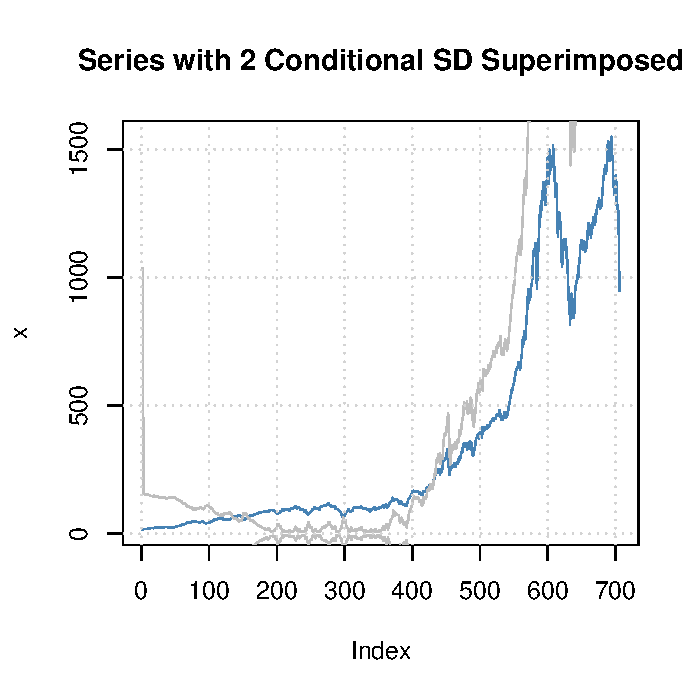
\includegraphics[scale=.8]{conditional-sd}
	\caption[S\&P 500 GARCH Estimate]{Monthly S\&P 500 GARCH Estimate with Two Conditional SD Superimposed}
	\label{figure:conditional-sd}
\end{figure}

\subsubsection{Integrated GARCH Model}\index{Integrated GARCH\\(IGARCH) model}
\margincomment[red]{IGARCH is a unit-root GARCH model.}
When AR polynomial of \eqref{eq:garch} has a unit root, then we have an IGARCH model.
The IGARCH(1,1) model
\begin{equation}
a_t = \sigma_t \epsilon_t, \quad \sigma^2_t = \alpha_0 + \beta_1 \sigma^2_{t-1} + (1-\beta_1)a^2_{t-1},
\label{eq:igarch}
\end{equation}
where $\{\epsilon_t\}$ is $1>\beta_1>0$. An IGARCH(1,1) model can be estimated by exponential smoothing methods when $\alpha_0=0$.

\subsubsection{GARCH in Mean Model}\index{GARCH in Mean\\(GARCH-M) model}
GARCH-M is a ``GARCH in the mean'' model because it adds the heteroskedastic term directly into the equation. It can be written as
\begin{eqnarray}
r_t &=& \mu + c\sigma^2_t + a_t, \quad a_t=\sigma_t \epsilon_t, \notag \\
\sigma^2_t &=& \alpha_0 + \alpha_1\alpha^2_{t-1} + \beta_1\sigma^2_{t-1},
\label{eq:garch-m}
\end{eqnarray}
where $\mu$ and $c$ are constants. The $c$ parameter is the \emph{risk premium parameter}. A $c>0$ indicates that the return has a positive relationship to its volatility.

\subsubsection{Exponential GARCH Model}\index{Exponential GARCH\\(EGARCH) model}
EGARCH was created to allow for asymmetric effects in asset returns. Positive and negative asset returns may not be equally symmetric, a problem not addressed by previous models. We begin with the weighted innovation
\[
g(\epsilon_t) = \theta \epsilon_t + \gamma \left[ |\epsilon_t| - E(|\epsilon_t|) \right],
\]
where $\theta$ and $\gamma$ are real constants. Both $\epsilon_t$ and $|\epsilon_t|-E(g(|\epsilon_t|)$ are zero-mean ($E[g(\epsilon_t)]$) iid sequences with continuous distributions. A better way to see the asymmetry is
\[
g(\epsilon_t) =
	\begin{cases}
	(\theta + \gamma)\epsilon_t - \gamma E(|\epsilon+t |) & \text{if $\epsilon_t \ge 0$,} \\
	(\theta - \gamma)\epsilon_t - \gamma E(|\epsilon+t |) & \text{if $\epsilon_t < 0$}.
	\end{cases}
\]
An EGARCH($m,s$) model can be written as
\begin{equation}
a_t = \sigma_t \epsilon_t, \quad \ln(\sigma^2_t)=\alpha_0 +
\frac{1+\beta_1 B+ \cdots +\beta_{s-1} B^{s-1}}{1-\alpha_1 B -\cdots -\alpha_m B^m} g(\epsilon_t - 1),
\label{eq:egarch}
\end{equation}
where $\alpha_0$ is a constant, $B$ is the \emph{back-shift} or lag operator such that $Bg(\epsilon_t)=g(\epsilon_{t-1})$, and $1+\beta_1 B +\cdots +\beta_{s-1} B^{s-1}$ and $1-\alpha_1 B -\cdots -\alpha_m B^m$ are polynomials with zeros outside the unit circle\footnote{To be \emph{outside the unit circle} means to have absolute values of the zeros greater than 1.} and have no common factors. The evolution of the conditional variance of $a_t$ is still contained in \eqref{eq:egarch} by using ARMA parameterization.

\paragraph{Alternative EGARCH Model.} An alternative form for EGARCH($m,s$) model is
\begin{equation}
\ln(\sigma^2_t) = \alpha_0 + \sum^s_{i=1} a_i \frac{|a_{t-i}|+\gamma_i a_{t-i}}{\sigma_{t-i}} +
\sum^m_{j=1} \beta_j \ln(\sigma^2_{t-j}).
\label{eq:egarch-alt}
\end{equation}
Notice in \eqref{eq:egarch-alt} that,
\begin{itemize}
\item a positive $a_{t-i}$ contributes $\alpha_i(1+\gamma_i)|\epsilon_{t-i}|$ to the log volatility,
\item a negative $a_{t-i}$ contributes $\alpha_i(1-\gamma_i)|\epsilon_{t-i}|$,
\end{itemize}
where $\epsilon_{t-i}=a_{t-i}/\sigma_{t-i}$. The leverage effect of $a_{t-i}$ is the $\gamma_i$ parameter.

\subsubsection{Conditional Heteroskedasticity (CHARMA) Model}\index{Conditional Heteroskedasticity\\(CHARMA) model}
The next model is CHARMA, which uses random coefficients to produce conditional heteroskedasticity. A CHARMA model is defined as
\begin{equation}
r_t = \mu_t + a_t, \quad a_t=\delta_{1t} a_{t-1} + \delta_{2t} a_{t-2} +\cdots +\delta_{mt} a_{t-m} + \eta_t,
\label{eq:charma}
\end{equation}
where $\{\eta_t\}$ is a Gaussian (normally distributed) white noise series with mean zero and variance $\sigma^2_{\eta}, \{\delta_t\}=\{(\delta_{1t}, \ldots,a_{mt})'\}$ is a sequence of iid random vectors with mean zero and non-negative definite covariance matrix $\mathbf{\Omega}$, and $\{\delta_t\}$ is independent of $\{\eta_t\}$.

The conditional variance of at of the CHARMA model \eqref{eq:charma} is
\begin{eqnarray}
\sigma^2_t &=& \sigma^2_{\eta} + \textbf{a}^{'}_{t-1} \text{Cov}(\delta)\textbf{a}_{t-1} \notag \\ 
&=& \sigma^2_t + (a, \ldots, a)\mathbf{\Omega}(a, \ldots, a).
\end{eqnarray}

\subsection{Stochastic Volatility Model}\index{Stochastic Volatility model}
If we model an underlying security's volatility as a random process, which is governed by state variables such as the price level of a security, there is a tendency of volatility to revert to some long-run mean value, and the variance of the volatility process itself.

Stochastic volatility models are one approach to resolve a shortcoming of some option pricing models that assume a fixed volatility during the life of the option contract. Because these option pricing models assume that the underlying volatility is constant over the life of the derivative, and unaffected by the changes in the price level of the underlying, they often misprice the option value. By assuming that the volatility of the underlying price is a stochastic process rather than a constant, it becomes possible to model derivatives more 
accurately.

The basic form of stochastic volatility is derived from Brownian motion, one of the simplest continuous-time stochastic processes, and is often used to model asset price movement.
\begin{equation}
dS_t = \mu S_t dt + \sigma S_t dW_t
\label{eq:brownian-motion}
\end{equation}

The maximum likelihood estimator to estimate the constant volatility $\sigma$, for given asset price time series $S_t$, at different times $t_i$, is 
\[
\hat{\sigma}^2= \left(\frac{1}{n} \sum_{i=1}^n \frac{(\ln S_{t_i}- \ln S_{t_{i-1}})^2}{t_i-t_{i-1}} \right) - \frac{1}{n} \frac{(\ln S_{t_n}- \ln S_{t_0})^2}{t_n-t_0}.
\]

\paragraph{GARCH Estimation.} The difficulty of estimating stochastic volatility is made slightly easier with GARCH methods, which assumes that the randomness of the variance process varies with the variance. The standard GARCH(1,1) model has this form for the variance differential
\[
d \nu_t = \theta(\omega - \nu_t )dt + \xi \nu_t dB_t .
\]

All stochastic volatility models have stochastic second moments (variance), but not all models that have stochastic second moments are called stochastic volatility models. Although stochastic volatility and GARCH are often presented as competing models, GARCH may help explain changes in volatility.

Both the ARCH/GARCH and stochastic volatility models derive their randomness 
from a white noise process. The difference is that an ARCH/GARCH process depends 
on just one white noise $W$. That white noise directly determines innovations in the ARCH/GARCH process while also indirectly determining innovations in its second moments. Despite the conventional description of \eqref{eq:brownian-motion}, stochastic volatility models generally depend on two white noise series, $V$ and $W$.

\paragraph{Heston model.} Another stochastic volatility model used for describing the evolution of the volatility of an underlying asset is the \emph{Heston model}\index{Heston model}. It assumes that the volatility of the asset is not constant, nor even deterministic, but follows a random process. Assuming that the asset price $S_t$ is determined by a stochastic process,
\[
dS_t = \mu S_t\,dt + \sqrt{\nu_t} S_t\,dW^S_t.
\]
The instantaneous variance is
\[
d\nu_t = \alpha(\theta - \nu_t)dt + \xi \sqrt{\nu_t}\,dW^{\nu}_t,
\]
where,
$\mu$ is the asset rate of return, $\theta$ is the long vol, or long run average price volatility; as $t$ tends to infinity, the expected value of $\nu_t$ tends to $\alpha$, $\alpha$ is the rate at which $\nu_t$ reverts to $\theta$, and $\xi$ is the volatility of the volatility (or, \emph{wiggle of the wiggle}), which determines the variance of $\nu_t$.

\section{Nonlinear Models}
\paragraph{Primary Text Reading.} \citeA[chap. 4]{tsay2005aft}\index{Tsay, Ruey} and \citeA{franses2000nlts}
\subsection{Simple Nonlinear Models}

Nonlinear data exists in \fts{}, especially in volatility and high-frequency data. We focus now on simple nonlinear models and neural networks. 

\paragraph{Bilinear Model.} A way to include rate-change points or other nonlinear events is to use a bilinear model such as
\begin{equation}
x_t = c+ \sum^p_{i=1} \phi_i x_{t-i} - \sum^q_{j=1} \theta_j a_{t-j} + \sum^m_{i=1} \sum^s_{j=1} \beta_{ij} x_{t-i} a_{t-j} + a_t,
\label{eq:bilinear}
\end{equation}
where $p,q,m,$ and $s$ are non-negative integers.

Some properties of bilinear models allow the modeling of nonlinear phenomenon with a minimum of parameters. 

\subsubsection{Threshold Autoregressive Model}\index{Threshold Autoregressive\\(TAR) Model} Adding some asymmetry to \eqref{eq:bilinear}, we have the threshold autoregressive model, which is a piecewise linear model in the threshold space. For example, a 2-regime AR(1) model 
\[
x_t =
\begin{cases}
-1.5x_{t-1} + a_t, &\text{if $x_{t-1}<0$,} \\
0.5x_{t-1} + a_t, &\text{if $x_{t-1} \ge 0$,}
\end{cases}
\]
where the $a_{t}$'s are iid $N(0, 1)$. 

Here the delay is 1 time period, $x_{t-1}$ is the threshold variable, and 
the threshold is 0. The threshold divides the $x_{t-1}$ space into two 
regimes with Regime 1 denoting $x_{t-1} < 0$.
% What is so special about this model? See the time plot in Tsay Figure 4.1. 

Special features of this model are,  (a) asymmetry in rising and declining 
patterns, (\textit{more observations are positive than are negative}) (b) the mean of $x_t$ is not zero even though there is no constant term in the model, and (c) the lag-1 coefficient may be greater than 1 in absolute value.

\subsubsection{Markov Switching Model}\index{Markov autoregressive\\switching (MSA) model}
Another example of a two-regime model, but with aperiodic switching is a two-state \emph{Markov autoregressive switching} (MSA) model is
\begin{equation}
x_t = 
\begin{cases}
c_1 + \sum^p_{i=1} \phi_{1,i} x_{t-i} + a_{1t}, &\text{if $s_t=1$,} \\
c_2 + \sum^p_{i=1} \phi_{2,i} x_{t-i} + a_{2t}, &\text{if $s_t=2$,}
\end{cases}
\end{equation} 
where $s_t$ assumes values in $\{1,2\}$ and is a first-order Markov chain 
with transition probabilities,
$P(s_t=2|s_{t-1}=1)=w_1, \quad P(s_t=1|s_{t-1}=2)=w_2,$
and where 0 $\le w_1 \le 1$ is the probability of switching out State 1 from 
time $t-1$ to time $t$. A large $w_1$ means that it is easy to switch out 
State 1, that is, it cannot stay in State 1 for long. The inverse, $1/w_1$, is 
the expected duration (\textit{number of time periods}) to stay in State 1. A similar idea applies to $w_2$. 

% TODO: Example See Figure 4.4 of the textbook (p.166)
% A good source is \citeA{franses2000nlts}.


\subsubsection{Nonparametric Methods}
There may be times when obtaining adequate information about the distribution will be impossible. In that case, we must rely upon nonparametric methods to perform estimation. They are very data dependent and may lead to over fitting of a model.

\margincomment{Kernel density estimators \emph{discover} the data's distribution.}
A major element of nonparametric methods is \emph{smoothing}. To do this, we need a density estimator, which is the construction of an estimate, based on observed data, of an unobservable underlying probability density function. The unobservable density function is thought of as the density according to which a large population is distributed; the data are usually thought of as a random sample from that population.

In MATLAB, kernel density estimation is implemented through the \texttt{ksdensity} function. The R language can perform this estimation using \texttt{density} function and the \texttt{kde2d} function, for two-dimensional kernel density estimation.

\paragraph{Kernel Regression.} Kernel regression is a non-parametric method to estimate the conditional expectation of a random variable. Its objective is to find a non-linear relationship between two random variables $x$ and $y$, such that
\[
E(y | x) = f(x)
\]
where $f$ is a non-parametric function. The relationship may also be expressed
\[
E(y | x) = \int y f(y|x) dy = \int y \frac{f(x,y)}{f(x)} dy.
\]
A common method is the Nadaraya-Watson kernel regression\index{Nadaraya-Watson kernel regression}, which is an estimate $m$ of a locally weighted average, using a kernel as a weighting function
\[
\widehat{m}(x)=\frac{\sum_{t=1}^T K_h(x-x_t)y_t }{\sum_{t=1}^T K_h(x-x_t)}.
\]

\subsubsection{Neural Networks}\index{Neural Networks}
Neural networks are non-linear statistical data modeling tools, often used to model complex relationships between inputs and outputs or to find meaningful patterns in data. Because of this, a neural network is a semi-parametric approach to data analysis. Neural networks learn by example. The analyst gathers representative data, and then invokes training algorithms to automatically learn the structure of the data. It has a network structure having,
\begin{itemize}
\item Input layer -- This is the observed data that we are trying to discover a relationship to. The aim is to find how known inputs and possibly known outputs are related.
\item Hidden layer -- The relationships between value pairs and the weights applied to them. Since the relationships may be complex, and be linked many ways through \emph{nodes}, there may multiple hidden layers. Sometimes, hidden layer is referred to in data mining literature as both a singular layer and as all layers collectively.
\item Nodes -- The mechanism that links layers together. Some neural network will have multiple hidden layers, and the way their layers are linked (through their nodes) will determine redundancy and search efficiency.
\item Output layer -- The resulting pairing from the input layer that have been paired through the hidden layer. Often, the analyst is uncertain how the pairing occurred, which runs the risk that out-of-sample data may behave differently, and thus, create a different hidden layer with different weightings.
\end{itemize}
The \emph{activation function}, which starts the network, is a logistic function,
\begin{equation}
\ell(z) = \frac{\exp(z)}{1+\exp(z)}
\label{eq:logistic}
\end{equation}
This function is plotted in Figure~\ref{figure:logistic} subject to $[-5,5]$.
\begin{figure}[tb]
	\centering
	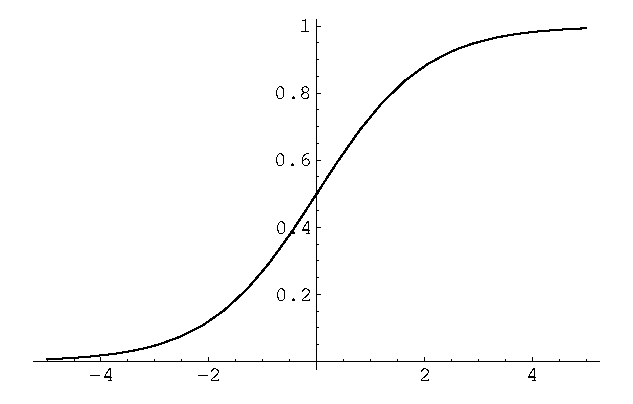
\includegraphics[scale=.8]{logistic}
	\caption{Plot of logistic function in \eqref{eq:logistic}}
	\label{figure:logistic}
\end{figure}
Next, the network requires the Heaviside (or threshold) function, which allows switching between regimes,
\[
H(z)=
\begin{cases}
1 &\text{if $z>0$,} \\
0 &\text{if $z \le 0$.}
\end{cases}
\]

A neural network having a hidden node works through,
\[
x_j = f_j(\alpha_j + \sum_{i \to j} w_{ij} x_i)
\]
where $f_j(\cdot)$ is an activation function which is typically taken to be 
the logistic function \eqref{eq:logistic}. Then, $\alpha_j$ is called the \emph{bias}, the summation $i \to j$ means summing over all input nodes feeding to $j$, and $w_{ij}$ are the weights.
The output node, 
\[
y=f_o(\alpha_o + \sum_{j \to o} w_{jo} x_j),
\]
where the activation function $f_o(\cdot)$ is either linear or a Heaviside 
function. By a Heaviside function, we mean $f_o(z) = 1$ if $z > 0$ and $f_o(z) = 0$, otherwise. Thus, the general form is,
\begin{equation}
y= f_o \Biggr[a_o + \sum_{j \to o} w_{jo} f_j \large( \alpha_j + \sum_{i \to j} w_{ij} x_i \large) \Biggr]
\end{equation}

\paragraph{Supervised Learning.} The task of knowledge discovery in databases (KDD)\index{Knowledge Discovery\\in Databases (KDD)} allows the analyst to examine data and its relationship to functional forms in two ways. The first, is through \emph{supervised learning}.  We have a set of data pairs $(x, y)$, $x \in X$, $y \in Y$ and the goal is to find a function $f$ within a class of functions that relates to the pairs. This ``supervised'' method requires us to infer how the mapping implied by the data and the cost function is related to the mismatch between our mapping and the data.

\paragraph{Unsupervised learning.} By contrast, through \emph{unsupervised learning} we are given some data $x$, and a cost function $c(\cdot)$ which is minimized with respect to any function of $x$ and the network's output, $f$. The cost function is determined by the task formulation. In this method, we have little, if any, idea how the data are related. We let the data make the connection for us.

\paragraph{Training and Forecasting.} Divide the data into training and forecasting subsamples. In the training subsample, build a few network systems. The forecasting is based on the accuracy of out-of-sample forecasts to select the ``best'' network. 

\subsection{Complex Nonlinear Models}

\subsubsection{Cosine Seasonality}
In some markets, seasonal energy markets, for instance, there may be at least two seasonal factors \cite{pilipovic2007er}\index{Pilipovic, Dragana}. The cosine function can capture these factors, requiring relatively few parameters -- the magnitude of the seasonal factor, and the time of year when it occurs. Here is a function that capture two different periodicities,

\begin{equation}
\overbrace{\beta_1 \cos(2 \pi (T-t^C_1))}^{annual} + \underbrace{\beta_2 \cos(4 \pi(T-t^C_2))}_{semi-annual}
\label{eq:cos-season}
\end{equation}
We can model two different seasonal patterns in \eqref{eq:cos-season} by representing $t^C_1$ with $\beta_1$ magnitude, as the annual center, and $t^C_2$ with $\beta_2$ magnitude, as the semi-annual center.

\subsubsection{Exponential Seasonality}
Using repetitive exponential functions is another way to model seasonality to capture a more narrow rise and fall of the \fts{}. This is different from the cosine function, in which the seasonal factor affects the entire curve. With exponential seasonality, we can apply local treatment,
\begin{equation}
\beta_1 \exp\Big({-\gamma_1 \big(rfc(T-t^C_1)\big)^2} \Big)+ \beta_2 \exp\Big({-\gamma_2 \big(rfc(T-t^C_2)\big)^2} \Big),
\label{eq:exp-season}
\end{equation}
where the function $rfc$ is annually repetitive, and returns the annualized time to or from the closest center $t^C_i$ for seasonal factor $i$. The two seasonal factors in \eqref{eq:exp-season} each has a center at $t^C$, a magnitude $\beta$, and a width of the seasonal peak defined by the ``decay'' coefficient $\gamma$.

%\subsection{Nonlinearity Testing}

%\subsubsection{Nonparametric Tests}

%\subsubsection{Parametric Tests}

%\subsection{Forecasting}

\section{High-Frequency Data Analysis}\label{High-Frequency}
\paragraph{Primary Text Reading.} \citeA[chap. 5]{tsay2005aft}\index{Tsay, Ruey}

\subsection{Nonsynchronous Trading}

Market microstructure: Why is it important? 
\begin{enumerate}
\item Important in market design \& operation, e.g. to compare different markets (NYSE vs NASDAQ) 
\item To study price discovery, liquidity, volatility, etc. 
\item To understand costs of trading 
\item Important in learning the consequences of institutional arrangements on observed processes, e.g. 
\begin{itemize}
\item Nonsynchronous trading 
\item Bid-ask bounce 
\item Impact of changes in tick size, after-hour trading, etc. 
\item Impact of daily price limits (many foreign markets) 
\end{itemize}
\end{enumerate}

Nonsynchronous trading: \index{Time Series!differing time periods}
Key implication: may induce serial correlations even when the underlying returns are iid. 

Setup: log returns ${r_t}$ are iid $(\mu, \sigma^2)$ 
For each time index $t$, P(no trade) = $\pi$. 
Cannot observe $r_t$ if there is no trade. 
What is the observed log return series $r^o_t$? 
It turns out $r^o_t$ is given in Tsay Eq. (5.1), 
% TODO: page 11 of lec7-08.pdf

\subsection{Bid-Ask Spread}

\subsection{Transaction Data}

\subsection{Price Change Models}

\subsubsection{Ordered Probit Model}

\subsubsection{Decomposition Model}

\subsection{Duration Models}

\subsubsection{ACD Model}

\subsubsection{Simulation}

\subsubsection{Estimation}

\subsection{Nonlinear Duration Models}


\section{Continuous-Time Models}
\paragraph{Primary Text Reading.} \citeA[chap. 6]{tsay2005aft}\index{Tsay, Ruey}

\paragraph{Discrete-Time Models.} Although it is observed that securities prices move in discrete ``ticks'', it is often convenient to view the \fts{} as \emph{continuous} function. There are some benefits to doing this. One of the main benefits is having a function on which can perform analysis -- get its derivative, for example, or make interpolations where missing data exists. However, this convenience comes at a cost. The mathematical complexity increases dramatically, and we require a different set of rules for \emph{real analysis}. Real analysis is the area of mathematics that studies concepts such as sequences and their limits, continuity, differentiation, integration and sequences of functions. 

\paragraph{Continuous-Time Stochastic Concepts.} We begin with the definition of a probability space $(\Omega, \mathcal{F}, \mathbb{P})$ where $\Omega$ is a nonempty space, $\mathcal{F}$ is a $\sigma$-field consisting of subsets of $\Omega$, and $\mathbb{P}$ is a probability measure.

Given a probability space $(\Omega, \mathcal{F}, \mathbb{P})$ and a measurable state space $(E, \mathcal{E})$, a stochastic process is a family $(X_t)t \geq 0$ such that $X_t$ is an $E$ valued random variable for each time
$t \geq 0$. For simplicity, we refer to a stochastic process as $\{x_t\}$, keeping in mind that $t$ is continuous.

\subsection{Wiener Process}\index{Wiener process}
In discrete-time mathematics, shocks form a white noise process, but in continuous-time, we use a \emph{Wiener process}, which is also known as \emph{standard Brownian motion}. Here is some R code for generating a Wiener process.
\ecaption{Wiener process in R}\index{R language}
\begin{verbatim}
n<-3000
epsi<-rnorm(n,0,1)
w=cumsum(epsi)/sqrt(n)
plot(w, type=`l')
\end{verbatim}
\margincomment[red]{Brownian motion variability increases with time.}
This is quite similar to the R code that generated Figure~\ref{figure:three-walks} \\ \texttt{plot(cumsum(rnorm(20000)),type=`l')}.

\paragraph{Martingales.}\index{martingales} A \emph{martingale} is a stochastic process, or a sequence of random variables, such that the conditional expected value of an observation at some time $t$, given all the observations up to some earlier time $s$, is equal to the observation at that earlier time $s$.

To produce a martingale in Excel is very simple. Enter 0 in cell A1. In cell A2 enter \texttt{=A1+NORMINV(RAND(),0,1)}. Copy cell A2 by dragging and creating 500 copies. This will create a martingale series with $\mu=0$ and $\sigma=1$. Notice that for the entire series $\mu \ne 0$ and $\sigma \ne 1$. This condition only applies at each time step. If a polynomial $f(x,t)$ satisfies the equation
\[
\Big( \frac{\partial}{\partial t} + \frac12 \frac{\partial^2}{\partial x^2} \Big) f(x,t) = 0,
\]
then the stochastic process $M_t = f ( W_t, t ) \,$ is a martingale, where $W_t$ is a Wiener process.

\subsection{It\^{o}'s Lemma}\index{It\^{o}'s lemma}
It\^{o}'s lemma starts with an \emph{It\^{o} process}, an adapted stochastic process which can be expressed as the sum of an integral with respect to Brownian motion and an integral with respect to time,
\begin{equation}
X_t=X_0+\int_0^t\sigma_s\,dB_s+\int_0^t\mu_s\,ds.
\label{eq:ito-process}
\end{equation}
where $B$ is a Brownian motion and it is required that $\sigma$ is a predictable $B$-integrable process, and $\mu$ is predictable and Lebesgue integrable, and any twice continuously differentiable function $f$ on the real numbers, then $f(X)$ is also an It\^{o} process satisfying
\begin{align}
df(X_t) &= f^\prime(X_t)\,dX_t + \frac{1}{2}f^{\prime\prime}(X_t)\sigma^2_t\,dt \notag \\
&= f^\prime(X_t)\sigma_t\,dB_t + \left(f^\prime(X_t)\mu_t+\frac{1}{2}f^{\prime\prime}(X_t)\sigma^2_t\right)\,dt. \notag
\end{align}

which by It\^{o}'s lemma
\begin{align}
df(t,X_t)&=\dot{f}(t,X_t)\,dt+f'(t,X_t)\,dX_t+\frac{1}{2}f''(t,X_t)\sigma^2_t\,dt, \notag \\ &=\dot{f}(t,X_t)\,dt+f'(t,X_t)(\mu_t\,dt + \sigma_t\,dB_t)+\frac{1}{2}f''(t,X_t)\sigma^2_t\,dt.
\end{align}

The lemma result is the stochastic calculus counterpart of the chain rule of Newtonian calculus, and it can be thought of as the Taylor series expansion and retaining the second order term related to the stochastic component change.

\subsection{Stochastic Differentials}
A \emph{stochastic differential equation}\index{stochastic differential equation} (SDE) is a differential equation where at least one of the terms is a stochastic process, resulting in a solution which is itself a stochastic process. Typically, SDEs incorporate white noise which can be thought of as the derivative of Brownian motion. However, it is worth mentioning that other types of random fluctuations are possible, such as jump processes, which we cover in Section~\ref{jump-diffusion}.

The typical form of an SDE is
\begin{equation}
\mathrm{d} X_t = \mu(X_t,t)\, \mathrm{d} t +  \sigma(X_t,t)\, \mathrm{d} B_t , 
\label{eq:sde-form}
\end{equation}
where $B$ is a Wiener process.

\paragraph{Example.} Assume that the price of a stock follows a geometric Brownian motion. What is the distribution of the log return? To answer this question, we need It\^{o} calculus. 

Let $G(x)$ be a differentiable function of $x$. 
What is $dG(x)$? \\
We begin with the Taylor expansion,
\[
\Delta G \equiv G(x+\Delta x)-G(x) = \frac{\partial G}{\partial x} \Delta x 
+ \frac{1}{2} \frac{\partial^2 G}{\partial x^2} (\Delta x)^2 +\frac{1}{6}\frac{\partial^3 g}{\partial x^3}(\Delta x)^3 + \cdots,
\]
Letting $\Delta x \to 0$, we have
\[
dG = \frac{\partial G}{\partial x}dx.
\]
Next, $G(x,y)$
\[
\Delta G =\frac{\partial G}{\partial x}\Delta x + \frac{\partial G}{\partial y}\Delta y + \frac{1}{2} \frac{\partial^2 G}{\partial x^2} (\Delta x)^2
+ \frac{\partial^2 G}{\partial x \partial y} \Delta x \Delta y + \frac{1}{2} \frac{\partial^2 G}{\partial y^2} (\Delta y)^2 + \cdots,
\]
Taking limits as $\Delta x \to 0$ and $\Delta y \to 0$, we have
\[
dG = \frac{\partial G}{\partial x}dx + \frac{\partial G}{\partial y}dy.
\]

\paragraph{Stochastic differentiation.} Now, consider $G(x_t , t)$ with $x_t$ being an It\^{o} process.
\[
\Delta G =\frac{\partial G}{\partial x}\Delta x + \frac{\partial G}{\partial t}\Delta t + \frac{1}{2} \frac{\partial^2 G}{\partial x^2} (\Delta x)^2
+ \frac{\partial^2 G}{\partial x \partial t} \Delta x \Delta t + \frac{1}{2} \frac{\partial^2 G}{\partial t^2} (\Delta t)^2 + \cdots,
\]
A discretized version of the It\^{o} process is
\[
\Delta x = \mu_* \Delta t + \sigma_* \epsilon \sqrt{\Delta t},
\]
where $\mu_*=\mu(x_t,t)$ and $\sigma_*=\sigma(x_t,t)$. Therefore,
\begin{eqnarray}
(\Delta x)^2 &=& \mu^2_*(\Delta t)^2+\sigma^2_* \epsilon^2 \Delta t + 2 \mu_*\sigma_*\epsilon(\Delta t)^{3/2} \notag \\
&=& \sigma^2_*\epsilon^2 \Delta t+H(\Delta t). \notag
\end{eqnarray}
Thus, $(\Delta x)^2$ contains a term of order $\Delta t$.
\begin{subequations}
\begin{eqnarray}
	E(\sigma^2_* \epsilon^2 \Delta t) &=& \sigma^2_* \Delta t, \label{eq:ito-E} \\
	\text{Var}(\sigma^2_* \epsilon^2 \Delta t) &=& E[\sigma^4_* \epsilon^4 (\Delta t)^2] - [E(\sigma^2_*\epsilon^2 \Delta t)]^2 = 2\sigma^4_*(\Delta t)^2, \label{eq:ito-Var}
\end{eqnarray}
\end{subequations}
where we use $E(\epsilon^4) = 3$. These two properties show that
\[
\sigma^2_* \epsilon^2 \Delta t \to \sigma^2_* \Delta t \quad \text{as} \quad \Delta t \to 0.
\]
Consequently,
\[
(\Delta x)^2 \to \sigma^2_* dt \quad \text{as} \quad \Delta t \to 0.
\]
With this result, we have
\begin{eqnarray}
dG &=& \frac{\partial G}{\partial x}dx + \frac{\partial G}{\partial t}dt + \frac{1}{2}\frac{\partial^2 G}{\partial x^2}\sigma^2_* dt \notag \\
&=& \Bigg( \frac{\partial G}{\partial x} \mu_* + \frac{\partial G}{\partial t} + \frac{1}{2} \frac{\partial^2 G}{\partial x^2}\sigma^2_* \Bigg) dt + \frac{\partial G}{\partial x} \sigma_* dw_t,
\label{eq:ito-lemma}
\end{eqnarray}
which is It\^{o}'s lemma. Now that we have the expected value \eqref{eq:ito-E}, and variance \eqref{eq:ito-Var}, we can determine the distribution of the log return.

\subsection{Stochastic Integrals}\index{stochastic integrals}
The rules of calculus, as defined by Newton, Leibniz, and others apply to a smooth function $f(x)$ where we can obtain the derivative $f'(x)$. This derivative is also the tangent line that intersects at exactly one point to $f(x)$. A Wiener process is always jagged, and finding a single tangent line that intersects with the line created by that process is impossible because it will intersect the line \emph{infinite} number of times.  Therefore, we need to modify the rules of calculus to adapt to the rules of Newtonian calculus, while still preserving some of the same concepts such as integration, as we saw in \eqref{eq:ito-lemma}.

The It\^{o} stochastic integral represents the payoff of a continuous-time  trading strategy consisting of holding an amount $H_t$ of the stock at time $t$, 
\[
Y_t=\int_0^t H_s\,dX_s.
\]
In this situation, the condition that $H$ is adapted corresponds to the necessary restriction that the trading strategy can only make use of the available information at any time. This prevents the possibility of unlimited gains through high frequency trading, that is, buying the stock just before each up-tick in the market and selling before each down-tick. Similarly, the condition that $H$ is adapted implies that the stochastic integral will not diverge when calculated as a limit of Riemann sums.

Important results of It\^{o} calculus include the integration by parts formula and It\^{o}'s lemma, which is a change of variables formula. These differ from the formulas of standard calculus, due to quadratic variation terms.

\subsection{Jump-Diffusion Model}\label{jump-diffusion}
When we view the activity of \fts{} in continuous time, we apply a \emph{diffusion model}, a concept borrowed from physics. In general, diffusion is the process whereby particles (\textit{or, in our case prices and asset returns}) intermingle as the result of their spontaneous movement caused by agitation (\textit{market forces}). This way, we can view prices and asset returns as ``particles'' moved in continuous random motion.

There are some weaknesses of diffusion models, which include,
\begin{itemize}
\item There is no \emph{volatility smile}, the convex function of implied volatility with respect to option strike
price,
\item Failure to capture effects of rare events in the distribution tails,
\item Prices sometimes open at significantly different levels than they close in the previous trading session.
\end{itemize}

Trying to combine both the phenomenon of ``jumps'' (\textit{the occasional non-continuous nature of market prices}) and continuous-time finance, we have the \emph{jump diffusion model}.
The simple jump diffusion model postulates that the price follows the stochastic differential equation, and is an extension to \eqref{eq:sde-form}. Jumps are governed by a probability law such as a Poisson process, where $X_t$ is a Poisson process if
\[
Pr(X_t=m) \frac{\lambda^m t^m}{m!}\exp(-\lambda t), \quad \lambda>0.
\]

We can use a special jump diffusion model,
\[
\frac{dP_t}{P_t}=\mu dt + \sigma dw_t + d \Bigg( \sum^{n_t}_{i=1}(J_i-1) \Bigg),
\]
where, \\
$w_t$ is a Wiener process, \\
$n_t$ is a Poisson process with rate $\lambda$, \\
$\{J_i\}$ is iid such that $X=\ln(J)$ has a double exponential distribution with pdf
\[
f_x(x) = \frac{1}{2\eta} e^{-|x-k|/\eta}, \quad 0<\eta<1.
\]
The above three processes are independent.
\section{Extreme Values \& Value at Risk}
\paragraph{Primary Text Reading.} \citeA[chap. 7]{tsay2005aft}\index{Tsay, Ruey}

\subsection{Value-at-Risk}\index{value-at-risk}
Value at Risk (VaR) is defined with respect to a specific portfolio of financial assets, at a specified probability and a specified time horizon. The probability that the mark-to-market loss on the portfolio over the time horizon is greater than VaR, assuming normal markets and no trading, is the specified probability level.

VaR tries to quantify two major items,
\begin{itemize}
\item a measure of minimum loss of a given asset
\item amount a position could decline in a given period, associated with a given probability (or confidence level)
\end{itemize}

For example, if a portfolio of stocks has a one-day 5\% VaR of \$1 million, there is a 5\% probability that the portfolio will decline in value by \emph{more than} \$1 million over the next day, assuming markets are normal and there is no trading. Such an event is termed a ``VaR break.''

\margincomment{Important ideas related to VaR are: economic capital, back-testing, stress testing and expected shortfall.}
VaR has five main uses in finance: risk management, risk measurement, financial control, financial reporting and computing regulatory capital. It is a simple measure, relatively speaking, but it has various methodologies, many of which are controversial. We start with some more formal definitions,
\begin{enumerate}
\item time period given: $\Delta t = \ell$
\item change in value: $\Delta V(\ell)$
\item cdf of the change: $F_{\ell}(x)$
\item given probability at tail: $p$
\item Long position
\[
p=Pr[\Delta V(\ell) \le \text{VaR}]=F_{\ell}(\text{VaR})
\]
\item Short position \\
\begin{eqnarray*}
p &=& Pr[\Delta V(\ell) \ge \text{VaR}] \\
&=& 1 - Pr[\Delta V(\ell) \le \text{VaR}] \\
&=& 1 - F_{\ell}(\text{VaR})
\end{eqnarray*}
\end{enumerate}
We can study VaR by simply focusing on the loss function and quantile $x_p$, the $p$th quantile of $F_{\ell}(x)$ if
$p=F_{\ell}(x_p)$ and $F_{\ell}(\cdot)$ is continuous.

There are several factors that affect VaR,
\begin{enumerate}
\item the probability $p$,
\item the time horizon $\ell$. One-week VaR will allow more swings, and thus, more losses, than a one-day VaR,
\item the cdf $F_{\ell}(x)$, the cdf of \emph{loss}. We can create a distribution of asset returns from historical data, but how well does the past work as an estimator for the future?
\item the \emph{mark-to-market} value of the position, which may be difficult to determine in some markets,
\item volatility $\sigma^2_t$ and how it is measured. \emph{RiskMetrics}, developed by J.P. Morgan, uses a special IGARCH model,
\[
\sigma^2_t = \alpha \sigma^2_{t-1}+(1-\alpha)r^2_{t-1}, \quad 1 > \alpha > 0.
\]
\end{enumerate}

One way of finding the predicted weekly losses at the 5th percentile is to generate a density from historic returns data, then find the 5\% level within the density estimate. The density is depicted in Figure~\ref{figure:SPW-VaR}.
\index{R language}\index{density@\texttt{density} (in R)} 
\begin{verbatim}
spxw<-read.csv("SPX-W.csv", header=T)
Log.Returns<-log(spxw$Close[2:NROW(spxw)]/
                 spxw$Close[1:(NROW(spxw)-1)])
ret.dens<-density(Log.Returns)
plot(ret.dens, "Density of S&P Log Returns")
ret.dens$x
ret.dens$x[NROW(ret.dens$x)*.05]
\end{verbatim}

\begin{figure}[tb]
  \centering
  \includegraphics[scale=.4]{SPW-VaR}
  \caption[S\&P 500 Density of Log Returns]{S\&P 500 Density of Log Returns to demonstrate 5\% one-week Value-at Risk }
  \label{figure:SPW-VaR}
\end{figure}

\begin{figure}[tb]
  \centering
  \includegraphics[scale=.72]{Est-VaR}
  \caption[Comparing Density of Log Returns]{Comparing a 5\% VaR for two assets using (a) density estimates and (b) normal distribution assumptions. Also, notice the normal distribution superimposed in panel (b) so that we get a better idea of the skewness and kurtosis of log returns for these two asset returns.}
  \label{figure:est-VaR}
\end{figure}

Some VaR methods will calculate the standard deviation and the mean of the log returns to generate a normal distribution. From that distribution, the analyst measures the value-at-risk at the fifth percentile to determine the 5\% VaR. In Figure~\ref{figure:est-VaR}, we compare a 5\% VaR for two assets using density estimates and normal distribution assumptions.

In Figure~\ref{figure:est-VaR}(a), we create a density estimate of the log returns, and in Figure~\ref{figure:est-VaR}(b), we obtain the mean and the standard deviation of the log returns and assume a normal distribution. The R code to perform these operations is listed.

\ecaption{Two methods of Calculating Historical VaR in R}\index{R language}
\begin{verbatim}
# 5% daily VaR quantile scores based on density estimate
aapl.VaR<-aapl.ret.dens$x[NROW(aapl.ret.dens$x)*.05]
gm.VaR<-gm.ret.dens$x[NROW(gm.ret.dens$x)*.05]

# NVaR: VaR drawn from a normal distribution sample.
aapl.NVaR<-qnorm(.05, mean(aapl.ret.dens$x), sd(aapl.ret.dens$x))
gm.NVaR<-qnorm(.05, mean(gm.ret.dens$x), sd(gm.ret.dens$x))
\end{verbatim}

\paragraph{VaR Controversies.} The use of VaR as risk management tool has been controversial since it moved from trading desks and into the public in 1994. A heated debate in 1997 between Nassim Taleb\index{Taleb, Nassim} and Philippe Jorion\index{Jorion, Philippe} set out some of the major points of contention. Taleb claimed that VaR,
\begin{enumerate}
\item ignored 2,500 years of experience in favor of untested models built by non-traders,
\item was ``charlatanism'' because it claimed to estimate the risks of rare events, which is impossible,
\item gave false confidence,
\item would be exploited by traders.
\end{enumerate}

More recently, David Einhorn\index{Einhorn, David} and Aaron Brown\index{Brown, Aaron} debated VaR in the publication, \emph{Global Association of Risk Professionals Review}. Einhorn compared VaR to ``an airbag that works all the time, except when you have a car accident.'' He further charged that VaR,
\begin{enumerate}
\item led to excessive risk-taking and leverage at financial institutions,
\item focused on the manageable risks near the center of the distribution and ignored the tails,
\item created an incentive to take ``excessive but remote risks'',
\item Was ``potentially catastrophic when its use creates a false sense of security among senior executives and watchdogs.''
\end{enumerate}

A common complaint among academics is that VaR is not \emph{subadditive}, which means that the VaR of a combined portfolio can be larger than the sum of the VaRs of its components. To a practicing risk manager this makes sense. For example, let us suppose the average portfolio suffers market correction, and faces a loss once every ten years. A single portfolio has approximately 0.004\% chance of facing a market correction loss on a specific day, so the risk of such a catastrophic loss would not figure into one-day 1\% VaR. It would not even be within an order of magnitude of that, so it is in the range where the institution should not worry about it.

\subsection{Extreme Value Theory}
In VaR, we are mostly focused on what happens at a predictable quantile, usually the 5th percentile within a specific time frame. In \emph{extreme value theory}, we focus upon the tail behavior of $r_t$. A properly normalized $r_{(1)}$ assumes a special distribution,
\[
F_*(x)=
\begin{cases}
1-\exp[-(1+kx)^{1/k}] & \text{if } k \ne 0 \\
1-\exp[-\exp(x)] & \text{if } k=0.
\end{cases}
\]
for $x<-1/k$ if $k<0$ and $x>-1/k$ if $k>0$,
where, \\
$k$ is the shape parameter, \\
$\alpha =-1/k$, the tail index of the distribution.

\clearpage
We have three different types of distributions to work with,
\begin{enumerate}
\item $k = 0$, the Gumbel family. The cdf is
\[
F_*(x)=1-\exp[-exp(x)], \quad -\infty < x < \infty.
\]
\item $k < 0$, the Fr\'{e}chet family. The cdf is
\[
F_*(x)=
\begin{cases}
1-\exp[-(1+kx)^{1/k}] & \text{if } x< -1/k, \\
1 & \text{otherwise.}
\end{cases}
\]
\item $k>0$, the Weibull family. The cdf is
\[
F_*(x)=
\begin{cases}
1-\exp[-(1+kx)^{1/k}] & \text{if } x>-1/k, \\
0 & \text{otherwise}.
\end{cases}
\]
\end{enumerate}

Here, we will demonstrate some functions of the \texttt{evir} library, ``Extreme Values in R'' \cite{evir-R}.
\ecaption{Extreme Values in R using Weibull, Fr\'{e}chet, \& Gumbel distributions}\index{R language}\index{evir@\texttt{evir} (library in R)}
\rpkg{evir}
\begin{verbatim}
library("evir")
# Generate CDF of Weibull, Frechet, & Gumbel dists
z=seq(-5,5,length=200)
# pgev to obtain the cdf of generalized extreme value dist.

# Frechet dist for z > -2 only, because xi=0.5.
cdf.f=ifelse((z > -2),pgev(z,xi=0.5),0)

# Weibull dist for z < 2 only.
cdf.w=ifelse((z < 2), pgev(z,xi=-0.5),1)

# Gumbel dist.
cdf.g=exp(-exp(-z))

plot(z,cdf.w,type=`l',xlab=`z',ylab=`H(z)')
lines(z,cdf.f,type=`l',lty=2)
lines(z,cdf.g,lty=3)
legend(-5,1,legend=c("Weibull H(-0.5,0,1)", "Frechet H(0.5,0.1)",
    "Gumbel H(0,0,1)"),lty=1:3)
\end{verbatim}
When you run this code, make sure you have a large enough graphics window so that the legend does not overlap the plots. There is an S version of \texttt{evir} called \texttt{evis}, which stands for ``Extreme Values in S''.

\subsection{Expected Shortfall}
Expected shortfall is a term used in financial risk management to evaluate the market risk of a portfolio. It is an alternative to Value-at-Risk. The ``expected shortfall at $q$\% level'' is the expected return on the portfolio in the worst $q$\% of the sampled cases. Expected shortfall is also called Conditional Value at Risk\index{conditional value-at-risk} (CVaR) and Expected Tail Loss\index{expected tail loss} (ETL).

ES evaluates the value \emph{or risk} of an investment in a more conservative way than VaR, focusing on the less profitable outcomes. For high values of $q$ it ignores the most profitable but unlikely possibilities, for small values of $q$ it focuses on the worst losses. On the other hand, unlike the discounted maximum loss even for lower values of $q$ expected shortfall does not consider only the single most catastrophic outcome. A value of $q$ often used in practice is 5\%.

Expected shortfall is a coherent, and moreover, a spectral measure of financial portfolio risk. It requires a quantile-level $q$, and is defined to be the expected loss of portfolio value given that a loss is occurring at or below the $q$-quantile. A major contributor to the theories of ES is Carlo Acerbi\index{Acerbi, Carlo}.

The expected loss given that the VaR is exceeded is \emph{Expected Shortfall} (ES). Specifically,
\[
\text{ES}_q = E(r|r>\text{VaR}_q) = \text{VaR}q + E(r-\text{VaR}_q|r>\text{VaR}_q).
\]
For GPD, it turns out that
\[
\text{ES}_q = \frac{\text{VaR}_q}{1+k} + \frac{\psi(\eta)+k\eta}{1+k}
\]

When we use the R library, \texttt{evir}, the command to generate VaR and ES is \texttt{riskmeasures}.

\section{Multivariate Time Series Analysis}
\paragraph{Primary Text Reading.} \citeA[chap. 8]{tsay2005aft}\index{Tsay, Ruey}

\section{Principal Component Analysis and Factor Models}
\paragraph{Primary Text Reading.} \citeA[chap. 9]{tsay2005aft}\index{Tsay, Ruey} and
\citeA{urga2007cfe}

\section{Multivariate Volatility Models}
\paragraph{Primary Text Reading.} \citeA[chap. 10]{tsay2005aft}\index{Tsay, Ruey}
and \citeA{lanne2007mgof}

Correlations between asset returns are important in many financial applications. In recent years, multivariate volatility models have been used to describe the time-varying feature of the correlations. However, the curse of dimensionality quickly becomes an issue as the number of correlations is $k(k -1)/2$ for $k$ assets \cite{tsay2006mvm}.

Let $\mathbf{r}_t = (r_{1t}, \ldots , r_{kt})$ be a vector of returns (or log returns) of $k$ assets at time index $t$. Let $\mathbf{F}_{t-1}$ be the sigma field generated by the past information at time index $t-1$. We partition the return $\mathbf{r}_t$ as
\begin{equation}
\mathbf{r}_t = \mu_t + e_t,
\end{equation}
where $\mu_t = E(r_t | \mathbf{F}_{t-1} )$ is the conditional mean of the return given $\mathbf{F}_{t-1}$ and $e_t$ is the innovation (\emph{or noise term}) satisfying $e_t = \sigma^{1/2}_t \epsilon_t$ such that 
\[
\text{Cov}(e_t | \mathbf{F}_{t-1} ) = \text{Cov}(r_t | \mathbf{F}_{t-1} ) = \Sigma_t,
\]
where $t = (\epsilon_{1t}, \ldots, \epsilon_{kt})'$ is a sequence of independently and identically distributed random vectors with mean zero and identity covariance matrix, and $\mathbf{\Sigma}^{1/2}_t$ is the symmetric square-root matrix of a positive-definite covariance matrix $\mathbf{\Sigma}_t$, that is, $\mathbf{\Sigma}^{1/2}_t \mathbf{\Sigma}^{1/2}_t = \mathbf{\Sigma}_t$. In the literature, $\mathbf{\Sigma}_t$ is often referred to as the volatility matrix. Volatility modeling is concerned with studying the evolution of the volatility matrix  over time. For asset returns, behavior of the conditional mean $\mu_t$ is relatively simple. 
In most cases, $\mu_t$ is simply a constant. In some cases, it may assume a simple vector autoregressive model. The volatility matrix $\mathbf{\Sigma}_t$, on the other hand, is much harder to model, and most GARCH studies in the literature focus entirely on modeling $\mathbf{\Sigma}_t$.

The conditional covariance matrix $\mathbf{\Sigma}_t$ can be written as 
\begin{equation}
\mathbf{\Sigma}_t = \mathbf{D}_t \mathbf{R}_t \mathbf{D}_t
\label{eq:cond-covar-matrix}
\end{equation}
where $\mathbf{D}_t$ is a diagonal matrix consisting of the conditional standard deviations of the returns, $\mathbf{D}_t = diag\{\sqrt{\mathbf{\Sigma}_{11},t}, \ldots, \sqrt{\mathbf{\Sigma}_{11},t}\}$ with $\mathbf{\Sigma}_{ij,t}$ being the $(i, j)$th element 
of $\mathbf{\Sigma}$, and $\mathbf{R}_t$ is the correlation matrix. 

\subsection{Vector Volatility Models} 
Many multivariate volatility models are available in the literature. In this section, we briefly review some of those models that are relevant to the proposed model. We shall focus on the simple models of order $(1, 1)$ in our discussion because such models are typically used in applications and the generalization to higher-order models is straightforward. In what follows, let $a_{ij}$ denote the $(i, j )$th element of the matrix $\mathbf{A}$ and $u_{it}$ be the $i$th element of the vector $\mathbf{u}_t$.

\subsection{Exponentially Weighted Estimates}
Given the innovations $\mathbf{F}_{t-1}=\{\mathbf{a}_1, \ldots,\mathbf{a}_{t-1}\}$, the unconditional covariance matrix of the innovation can be estimated by
\[
\widehat{\mathbf{\Sigma}}=\frac{1}{t-1} \sum^{t-1}_{j=1}\mathbf{a}_j\mathbf{a}'_j,
\]
where it is understood that the mean of $\mathbf{a}_j$ is zero. This estimate assigns equal weight $1/(t-1)$ to each term in the summation. To allow for a time-varying covariance matrix and to emphasize that recent innovations are more relevant, one can use the idea of exponential smoothing and estimate the covariance matrix of $\mathbf{a}_t$ by
\begin{equation}
\widehat{\mathbf{\Sigma}}_t=\frac{1-\lambda}{1-\lambda^{t-1}} \sum^{t-1}_{j=1}\lambda^{j-1} \mathbf{a}_{t-j}\mathbf{a}'_{t-j},
\label{eq:expon-wt-est}
\end{equation}
where $0< \lambda< 1$ and the weights $(1-\lambda)\lambda^{j-1}/ (1-\lambda^{t-1})$ sum to one. For a sufficiently large $t$ such that $\lambda^{t-1} \approx 0$, the prior equation can be rewritten as
\[
\widehat{\mathbf{\Sigma}}=(1-\lambda)\mathbf{a}_{t-1}\mathbf{a}'_{t-1} + \lambda \widehat{\mathbf{\Sigma}}_{t-1}.
\]
The covariance estimate in \eqref{eq:expon-wt-est} is referred to as the \emph{exponentially weighted moving average} (EWMA) estimate of the covariance matrix.

\subsection{Multivariate GARCH Models}
Just as we have been able to specify a \emph{univariate} GARCH model previously in Section~\ref{garch-spec}, we can examine some \emph{multivariate} GARCH models. Likewise, regression methods exist for either kind of model. Two nonparametric tests for investigating multivariate regression functions can be found in \citeA{RePEc:eee:econom:v:147:y:2008:i:1:p:151-162}.

\subsubsection{VEC Model}\index{VEC model} For a symmetric $n \times n$ matrix $\mathbf{A}$, let $\text{vech}(\mathbf{A})$ be the half-stacking vector of $\mathbf{A}$, that is, $\text{vech}(\mathbf{A})$ is a $n(n +1)/2 \times 1$ vector obtained by stacking the lower triangular portion of the matrix $\mathbf{A}$. Let $h_t = \text{vech}(\mathbf{\Sigma}_t)$ and $\eta_t = \text{vech}(e_t e'_t)$. Using the idea of exponential smoothing, the VEC model
\begin{equation}
h_t = c + \mathbf{A}_{\eta_t-1} + \mathbf{B}_{ht-1}
\label{eq:vec-model}
\end{equation}
where $c$ is a $k(k + 1)/2$ dimensional vector, and $\mathbf{A}$ and $\mathbf{B}$ are $k(k + 1)/2 \times k(k + 1)/2$ matrices. This model contains several weaknesses. First, the model contains $k(k + 1)[k(k + 1) + 1]/2$ parameters, which is large even for a small $k$. For instance, if 
$k = 3$, then the model contains 78 parameters, making it hard to apply in practice. To overcome this difficulty, it is suggested that both $\mathbf{A}$ and $\mathbf{B}$ matrices of \eqref{eq:vec-model} are constrained to be diagonal. The second weakness of the model is that the resulting volatility matrix $\mathbf{\Sigma}_t$ may not be positive definite.

\subsubsection{BEKK Model}\index{BEKK model}
\margincomment{BEKK is named for Baba, Engle, Kraft, and Kroner}
A simple BEKK model assumes the form
\begin{equation}
\mathbf{\Sigma}_t = \mathbf{C}'\mathbf{C} + \mathbf{A}' e_{t-1} e'_{t-1} \mathbf{A}+\mathbf{B}' \mathbf{\Sigma}_{t-1} \mathbf{B}
\label{eq:bekk}
\end{equation}
where $\mathbf{C}$, $\mathbf{A}$, and $\mathbf{B}$ are $k \times k$ matrices but $\mathbf{C}$ is upper triangular. An advantage of the BEKK model is that $\mathbf{\Sigma}_t$ is positive definite if the diagonal elements of $\mathbf{C}$ is positive. On the other hand, the model contains many parameters that do not represent directly the impact of $e_{t-1}$ or $\mathbf{\Sigma}_{t-1}$ on the elements of $\mathbf{\Sigma}_t$. In other words, it is 
hard to interpret the parameters of a BEKK model. Limited experience also shows that many parameter estimates of the BEKK model in \eqref{eq:bekk} are statistically insignificant, implying that the model is overparameterized. 

Using the standardization of \eqref{eq:cond-covar-matrix}, one can divide the multivariate volatility modeling into two steps. The first step is to specify models for elements of the $\mathbf{D}_t$ matrix, and the second step is to model the correlation matrix $\mathbf{R}_t$ . Two such approaches have been proposed in the literature. In both cases, the elements $\sigma_{ii,t}$ are assumed to follow a univariate GARCH model. In other words, $\sigma_{ii,t}$ are based entirely on the $i$-th return series. 

The individual volatility $\sigma_{ii,t}$ can assume any univariate GARCH models, and the correlation matrix $\mathbf{R}_t$ of \eqref{eq:cond-covar-matrix} follows the model
\begin{equation}
\mathbf{R}_t = (1-\lambda_1 -\lambda_2)\mathbf{R} + \lambda_1 \Psi_{t-1} + \lambda_2 \mathbf{R}_{t-1}
\label{eq:dyn-corr}
\end{equation}
where $\lambda_1$ and $\lambda_2$ are non-negative parameters satisfying $0 \le \lambda_1 + \lambda_2 < 1$, $\mathbf{R}$ is a $k \times k$ positive definite parameter matrix with $\mathbf{R}_{ii} = 1$ and $\Psi_{t-1}$ is the $k \times k$ correlation matrix of some recent asset returns. For instance, if the most recent $m$ returns are 
used to define $\Psi_t-1$, then the $(i, j )$th element of $\Psi_{t-1}$ is given by
\[
\Psi_{ij,t-1} = \frac{\sum^m_{v=1}u_{i,t-v}u_{j,t-v}}{\sqrt{\sum^m_{v=1}u^2_{i,t-v} u^2_{i,t-v}}}  
\]
where $u_{it} = e_{it} / \sqrt{\sigma{ii,t}}$ . If $m > k$, then $\Psi_t-1$ is positive definite almost surely. This in turn implies that $\mathbf{R}_t$ is positive definite almost surely. We refer to this model as a $DCC_T(m)$ model. In practice, one can use the sample correlation matrix of the data to estimate $\mathbf{R}$ in order to simplify the calculation. Indeed, this is the approach we shall take.

From the definition, the use of $DCC_T(m)$ model involves two steps. In the first step, univariate GARCH models are built for each return series. At step 2, the correlation matrix $\mathbf{R}_t$ \eqref{eq:cond-covar-matrix} is estimated across all return series via the maximum likelihood method. An advantage of the $DCC_T (m)$ model is that the resulting correlation matrices are positive definite almost surely. In addition, the model is parsimonious in parameterization because the evolution of correlation matrices is governed by two parameters. On the other hand, strong limitation is imposed on the time evolution of the correlation matrices. In addition, it is hard to interpret the results of the two-step estimation. For instance, it is not clear what is the joint distribution of the innovation e of the return series. 

We can demonstrate a concept using the R environment. In this case, we can use \texttt{mgarchBEKK}, although the package is in development, and only has full support in the Unix environment.
\rpkg{mgarchBEKK}

\subsection{Reparameterization}
Because $\mathbf{\Sigma}_t$ is a symmetrical matrix, we have two options for \emph{reparameterization}. These methods allow us to alter the parameter correlation in order to make a better-fitting model.

\subsubsection{Correlation Reparameterization}
Our first method allows us to reparameterize using the conditional coffecients and variances of $\mathbf{a}_t$, and we can write $\mathbf{\Sigma}_t$ as
\[
\mathbf{\Sigma}_t \equiv [\sigma_{ij,t}] = \mathbf{D}_t \mathbf{\rho}_t \mathbf{D}_t,
\]
where $\mathbf{\rho}_t$ is the conditional correlation matrix of $\mathbf{a}_t$ and $\mathbf{D}_t$ is a $k \times k$ diagonal matrix consisting of the conditional standard deviations of elements of $\mathbf{a}_t$, which is,
\[
\mathbf{D}_t = \text{diag}\Big( \{\sqrt{\sigma_{11,t}}, \ldots, \sqrt{\sigma_{kk,t}} \} \Big).
\]

However, as the matrix $\mathbf{\Sigma}_t$ gets large, it requires parameter constraints, and the function becomes increasingly complicated.

\subsubsection{Cholesky Decomposition}\index{Cholesky decomposition}
Because $\mathbf{\Sigma}_t$ is positive definite, there is a lower triangle matrix $\mathbf{L}_t$ with unit diagonal elements and a diagonal matrix $\mathbf{G}_t$ with positive diagonal elements such that
\begin{equation}
\mathbf{\Sigma}_t = \mathbf{L}_t \mathbf{G}\mathbf{L}'_t,
\label{eq:cholesky-decomp}
\end{equation}
which is the \emph{Cholesky decomposition} of $\mathbf{\Sigma}_t$.

% Might be good to include the matrices from Tsay, pp.455-456.

% \subsection{GARCH Models for Bivariate Returns}
%\paragraph{Constant-Correlation Models.}

\subsection{Higher Dimension Volatility}

In some situations, matrix multiplication in vector models such as these may rely upon a \emph{Kronecker product}, which is $(\mathbf{A}_i \otimes \mathbf{A}_i)'$.\index{Kronecker product}

If $\mathbf{A}$ is an $m$-by-$n$ matrix and $\mathbf{B}$ is a $p \times q$ matrix, then the Kronecker product $\mathbf{A}\otimes\mathbf{B}$ is the $mp \times nq$ block matrix
\[
\mathbf{A}\otimes\mathbf{B} = \begin{bmatrix} a_{11} B & \cdots & a_{1n}B \\ \vdots & \ddots & \vdots \\ a_{m1} B & \cdots & a_{mn} B \end{bmatrix}. 
\]
More explicitly, we have
\[
\mathbf{A}\otimes\mathbf{B} = \begin{bmatrix}    a_{11} b_{11} & a_{11} b_{12} & \cdots & a_{11} b_{1q} &                     \cdots & \cdots & a_{1n} b_{11} & a_{1n} b_{12} & \cdots & a_{1n} b_{1q} \\    a_{11} b_{21} & a_{11} b_{22} & \cdots & a_{11} b_{2q} &                     \cdots & \cdots & a_{1n} b_{21} & a_{1n} b_{22} & \cdots & a_{1n} b_{2q} \\    \vdots & \vdots & \ddots & \vdots & & & \vdots & \vdots & \ddots & \vdots \\    a_{11} b_{p1} & a_{11} b_{p2} & \cdots & a_{11} b_{pq} &                     \cdots & \cdots & a_{1n} b_{p1} & a_{1n} b_{p2} & \cdots & a_{1n} b_{pq} \\    \vdots & \vdots & & \vdots & \ddots & & \vdots & \vdots & & \vdots \\    \vdots & \vdots & & \vdots & & \ddots & \vdots & \vdots & & \vdots \\    a_{m1} b_{11} & a_{m1} b_{12} & \cdots & a_{m1} b_{1q} &                     \cdots & \cdots & a_{mn} b_{11} & a_{mn} b_{12} & \cdots & a_{mn} b_{1q} \\    a_{m1} b_{21} & a_{m1} b_{22} & \cdots & a_{m1} b_{2q} &                     \cdots & \cdots & a_{mn} b_{21} & a_{mn} b_{22} & \cdots & a_{mn} b_{2q} \\    \vdots & \vdots & \ddots & \vdots & & & \vdots & \vdots & \ddots & \vdots \\    a_{m1} b_{p1} & a_{m1} b_{p2} & \cdots & a_{m1} b_{pq} &                     \cdots & \cdots & a_{mn} b_{p1} & a_{mn} b_{p2} & \cdots & a_{mn} b_{pq}  \end{bmatrix}. 
\]

To demonstrate the difference between matrix multiplication introduced in Section~\ref{linear-algebra} and a Kronecker product, note the following,
\[
\begin{bmatrix}
	1 & 2 \\
	3 & 4 \\
\end{bmatrix}
\otimes
\begin{bmatrix}
      0 & 5 \\
      6 & 7 \\
\end{bmatrix} =
\begin{bmatrix}
	1\cdot 0 & 1\cdot 5 & 2\cdot 0 & 2\cdot 5 \\
	1\cdot 6 & 1\cdot 7 & 2\cdot 6 & 2\cdot 7 \\      
	3\cdot 0 & 3\cdot 5 & 4\cdot 0 & 4\cdot 5 \\      
	3\cdot 6 & 3\cdot 7 & 4\cdot 6 & 4\cdot 7 \\    
\end{bmatrix}  =
\begin{bmatrix}
	0 & 5 & 0 & 10 \\      
	6 & 7 & 12 & 14 \\     
	0 & 15 & 0 & 20 \\     
	18 & 21 & 24 & 28
\end{bmatrix}
\]

which, when we use variables instead, is,
\[
\begin{bmatrix} a_{11} & a_{12} \\ a_{21} & a_{22} \\ a_{31} & a_{32} \end{bmatrix} \otimes \begin{bmatrix} b_{11} & b_{12} & b_{13} \\ b_{21} & b_{22} & b_{23} \end{bmatrix} = \begin{bmatrix} a_{11} b_{11} & a_{11} b_{12} & a_{11} b_{13} & a_{12} b_{11} & a_{12} b_{12} & a_{12} b_{13} \\ a_{11} b_{21} & a_{11} b_{22} & a_{11} b_{23} & a_{12} b_{21} & a_{12} b_{22} & a_{12} b_{23} \\ a_{21} b_{11} & a_{21} b_{12} & a_{21} b_{13} & a_{22} b_{11} & a_{22} b_{12} & a_{22} b_{13} \\ a_{21} b_{21} & a_{21} b_{22} & a_{21} b_{23} & a_{22} b_{21} & a_{22} b_{22} & a_{22} b_{23} \\ a_{31} b_{11} & a_{31} b_{12} & a_{31} b_{13} & a_{32} b_{11} & a_{32} b_{12} & a_{32} b_{13} \\ a_{31} b_{21} & a_{31} b_{22} & a_{31} b_{23} & a_{32} b_{21} & a_{32} b_{22} & a_{32} b_{23} \end{bmatrix}
\]

%\subsection{Factor Volatility Models}

\subsection{Eigenvalue Example Using Fixed Income Scenarios}
To demonstrate using principal component analysis\index{principal component analysis} and eigenvalue decomposition\index{eigenvalue decomposition} in Monte Carlo simulation of a yield curve comprising several fixed income instruments, we turn to an example in \citeA{marrison2002frm}. To begin, consider a U.S. government yield curve. We have statistics in the following matrices: standard deviation $\mathbf{S}$, correlation $\mathbf{R}$, and covariance $\mathbf{C}$ for absolute changes in the 3-month, 1-year, 5-year, and 20-year interest rates. Using these matrices, we want to create a matrix $\mathbf{B}$ that will assist us in creating random scenarios.

\begin{eqnarray*}
\mathbf{S} &=&
\begin{bmatrix}
	0.051 & 0.052 & 0.061 & 0.054
\end{bmatrix} \\
\\
\mathbf{R} &=&
\begin{bmatrix}
	1 & 0.61 & 0.42 & 0.31 \\
	0.61 & 1 & 0.83 & 0.67 \\
	0.42 & 0.83 & 1 & 0.88 \\
	0.31 & 0.67 & 0.88 & 1
\end{bmatrix} \\
\\
\mathbf{C} &=& \text{diag}(S) \times R \times \text{diag}(S)
%\mathbf{C} &=& \mathbf{S}^T \mathbf{R}\mathbf{S} \\
\\
&=&
\begin{bmatrix}
	.0026 & .0016 & .0013 & .0008 \\
	.0016 & .0027 & .0026 & .0019 \\
	.0013 & .0026 & .0038 & .0029 \\
	.0008 & .0019 & .0029 & .0029
\end{bmatrix}.
\end{eqnarray*}
We obtain the eigenvalue decomposition of $\mathbf{C}$ in MATLAB or Octave using,
\ecaption{Eigenvalue Decomposition in MATLAB}
\begin{verbatim}
    lambda_sqrt = sqrt(eig(C));
    eigv_decom=diag(lambda_sqrt)
\end{verbatim}

\[
\mathbf{\Lambda}^{1/2}=
\begin{bmatrix}
	0.017804 & 0 & 0 &  0 \\
	0 & 0.024739 & 0 &  0 \\
	0 & 0 & 0.046721 & 0 \\
	0 & 0 & 0 & 0.094277 \\
\end{bmatrix}
\]
Eigenvectors have special properties that are useful for speeding up Monte Carlo simulations. Each eigenvector defines a market movement that is by definition independent of the other movements, because $\mathbf{I}=\mathbf{E}^T\mathbf{E}$. Also, $\mathbf{C}=\mathbf{E}^T \text{diag}(\mathbf{\Lambda}) \mathbf{E}$. Our $\mathbf{E}$ matrix is,
\[
\mathbf{E}=
\begin{bmatrix}
	\phantom{-}0.097 & -0.480 & \phantom{-}0.724 & -0.486 \\
	\phantom{-}0.407 & -0.694 & -0.124 & \phantom{-}0.581 \\
	-0.847 & -0.195 & \phantom{-}0.264 & \phantom{-}0.417 \\
	\phantom{-}0.327 & \phantom{-}0.500 & \phantom{-}0.625 & \phantom{-}0.502 \\
\end{bmatrix}
\]
How do we know this is an $\mathbf{E}$ matrix? Because \texttt{abs(round(transpose(E)*E))} makes a $4 \times 4$ identity matrix. Finally, we compute $\mathbf{B}=\mathbf{\Lambda}^{1/2} \mathbf{E}$,
\[
\mathbf{B}=
\begin{bmatrix}
	\phantom{-}0.0017269 & -0.0085457 & \phantom{-}0.0128898 & -0.0086525 \\
	\phantom{-}0.0100687 & -0.0171688 & -0.0030676 & \phantom{-}0.0143733 \\
	-0.0395723 & -0.0091105 & \phantom{-}0.0123342 & \phantom{-}0.0194825 \\
	\phantom{-}0.0308287 & \phantom{-}0.0471387 & \phantom{-}0.0589233 & \phantom{-}0.0473272
\end{bmatrix}
\]
We have four principal components, named \emph{wiggle}, \emph{flex}, \emph{twist}, and \emph{shift}. We can use the matrix $\mathbf{B}$ to create random scenarios,
\[
\begin{bmatrix}
\delta r_{3mo} & \delta r_{1yr} & \delta r_{5yr} & \delta r_{20yr}
\end{bmatrix}
=
\begin{bmatrix}
z_1 & z_2 & z_3 & z_4
\end{bmatrix}
\times \mathbf{B}.
\]
where $z_n$ is a random number generated for factor $n$. Each row of $\mathbf{B}$ describes its sensitivity to changes in the factor and the rate point,
\begin{eqnarray*}
wiggle &=& z_1 
\begin{bmatrix}
\phantom{-}0.0017269 & -0.0085457 & \phantom{-}0.0128898 & -0.0086525
\end{bmatrix}\\
flex &=& z_2
\begin{bmatrix}
\phantom{-}0.0100687 & -0.0171688 & -0.0030676 & \phantom{-}0.0143733
\end{bmatrix} \\
twist &=& z_3
\begin{bmatrix}
-0.0395723 & -0.0091105 & \phantom{-}0.0123342 & \phantom{-}0.0194825
\end{bmatrix} \\
shift &=& z_4
\begin{bmatrix}
\underbrace{\phantom{-}0.0308287}_{3mo} & \underbrace{\phantom{-}0.0471387}_{1yr} & \underbrace{\phantom{-}0.0589233}_{5yr} & \underbrace{\phantom{-}0.0473272}_{20yr}
\end{bmatrix}.
\end{eqnarray*}
We can see that for any given change in $z_n$, the \emph{shift} has the strongest effect, and \emph{wiggle} is the weakest.

For instance, if $z_4$ increases by 1, all of the rate points shift up by the magnitude of the bottom row of $\mathbf{B}$, which means the 3-month rate increases by 3 bps, the 1-year by 5 bps, the 5-year by 6 bps, and the 20-year by 5 bps. Notice that a positive change of 1 to $z_3$ would cause \emph{twist} in the 3-month rate to decrease 4 bps, and the 1-year to decrease 1 bp, but the 5- and 20-year rates increase 1 and 2 bps, respectively.

Since \emph{wiggle} and \emph{flex} have the least amount of influence, if we wanted to optimize our Monte Carlo simulation by reducing the number of random variables, we could hold $z_1$ and $z_2$ constant, and let $z_3$ and $z_4$ be random.

Imagine a process where we capture thousands of iterations of the following simulations. We will hold \emph{wiggle} and \emph{flex} constant, and will apply random shocks to \emph{twist} and \emph{shift}. We set $m$ to the magnitude of the random shock, and use \texttt{normrnd} to generate a normally-distributed random number with $\mu=0$ and $\sigma=1$.
\ecaption{Yield Curve Shocks in MATLAB}
\begin{verbatim}
    m=2
    round([1 1 m*normrnd(0,1) m*normrnd(0,1)]*(100*B))
\end{verbatim}
This gives us a row vector of basis point shocks for each rate point. For example, in one trial, the rate shocks $\delta r$ were obtained.
\[
\underbrace{-3 \text{ bps}}_{3mo} \quad \underbrace{-2 \text{ bps}}_{1yr} \quad \underbrace{6 \text{ bps}}_{5yr} \quad \underbrace{8 \text{ bps}}_{20yr}.
\]

\section{State-Space Models and Kalman Filters}
\paragraph{Primary Text Reading.} \citeA[chap. 11]{tsay2005aft}\index{Tsay, Ruey}

\section{Markov Chain Monte Carlo Methods}
\paragraph{Primary Text Reading.} \citeA[chap. 12]{tsay2005aft}\index{Tsay, Ruey}


%\addcontentsline{toc}{section}{References}
\bibliographystyle{apacite}
\bibliography{msf566-notes}

\clearpage
\addcontentsline{toc}{section}{Index}
\markright{Index}
\printindex
\end{document} 